% ****** Start of file randomized_encoding_qml.tex ******
%
% Modified manuscript draft: randomized-encoding implementation of input-level
% symmetry averaging for quantum machine learning.
%
\documentclass[%
 reprint,
 amsmath,amssymb,
 aps,
 pra,
]{revtex4-2}

\usepackage[utf8]{inputenc}
\usepackage{graphicx}
\usepackage{dcolumn}
\usepackage{bm}
\usepackage{algorithm}
\usepackage{algpseudocode}
\usepackage{multirow}
\usepackage{braket}
\usepackage{amsmath, amssymb, amsthm}
\usepackage{xcolor}
\usepackage{hyperref}
\usepackage[caption=false]{subfig}
\usepackage{orcidlink}
% \usepackage{tabularx}
% \usepackage{array}

\hypersetup{
    colorlinks=true,
    allcolors=blue
}

\newtheorem{theorem}{Theorem}
\newtheorem{proposition}[theorem]{Proposition}
\newtheorem{lemma}[theorem]{Lemma}
\newtheorem{corollary}[theorem]{Corollary}
\theoremstyle{definition}
\newtheorem{definition}[theorem]{Definition}

\iftrue
% display comments
\newcommand{\comments}[1]{\footnote{\textcolor{blue}{\textit{#1}}}}
\newcommand{\AL}[1]{\textcolor{green}{#1}}
\newcommand{\LW}[1]{\textcolor{blue}{#1}}
\newcommand{\SK}[1]{\textcolor{red}{#1}}
\newcommand{\ZT}[1]{\textcolor{magenta}{#1}}
\else
% do NOT display comments
\newcommand{\comments}[1]{}
\newcommand{\AL}[1]{#1}
\newcommand{\LW}[1]{#1}
\newcommand{\SK}[1]{#1}
\newcommand{\ZT}[1]{#1}
\fi

\usepackage{thmtools}
\newenvironment{restate}[2]{%
  \par\noindent\textbf{#1 \ref{#2}. }\itshape%
}{\par\medskip}

\begin{document}

\preprint{APS/123-QED}

\title{Resource-Efficient Symmetry Averaging for Quantum Machine Learning via Randomized Encoding}

\author{Letao Wang\,\orcidlink{0009-0004-2411-8916}}
% \email{letao.wang@centralesupelec.fr}
\affiliation{Laboratory of Signals and Systems, CentraleSup\'elec, CNRS,
Paris-Saclay University, 3 Rue Joliot Curie, Gif-sur-Yvette, 91190,
\^Ile-de-France, France}

\author{Abdel Lisser}
\affiliation{Laboratory of Signals and Systems, CentraleSup\'elec, CNRS,
Paris-Saclay University, 3 Rue Joliot Curie, Gif-sur-Yvette, 91190,
\^Ile-de-France, France}

\author{Sreejith Sreekumar}
\affiliation{Laboratory of Signals and Systems, CentraleSup\'elec, CNRS,
Paris-Saclay University, 3 Rue Joliot Curie, Gif-sur-Yvette, 91190,
\^Ile-de-France, France}

\author{Zeno Toffano}
\affiliation{Laboratory of Signals and Systems, CentraleSup\'elec, CNRS,
Paris-Saclay University, 3 Rue Joliot Curie, Gif-sur-Yvette, 91190,
\^Ile-de-France, France}

\date{\today}

\begin{abstract}
Symmetries provide important inductive biases for quantum machine learning, but enforcing them at the circuit level can require nontrivial quantum resources. Existing geometric quantum machine learning constructions often impose invariance or equivariance through symmetry-compatible embeddings, ansatz layers, observables, or twirling over quantum group representations. While these approaches are general, implementing the corresponding representation circuits can increase depth, require additional controls, or introduce hardware-dependent compilation overhead. In this work, we study a resource-efficient alternative for data-encoding quantum models in which the symmetry acts on the classical input before quantum encoding. Rather than applying a sampled quantum representation \(R(s)\) on hardware, we sample a symmetry transformation and encode the transformed input directly. This randomized-encoding implementation realizes the same input-averaged invariant predictor without additional qubits or quantum depth beyond the baseline circuit. We prove that the resulting estimator is unbiased, characterize its variance and shot-complexity trade-off, and compare its resource requirements with deterministic and stochastic twirling. We further analyze the effect of symmetry averaging in the Fourier representation of data re-uploading quantum models, showing how frequency orbits aggregate Fourier coefficients and can mitigate vanishing expressivity. As an application, we use sign-flip averaging to obtain quantum Chebyshev models for physics-informed learning, eliminating non-polynomial terms that arise from direct Chebyshev encodings.
\end{abstract}

\maketitle

\section{Introduction}

Many scientific and engineering problems possess intrinsic symmetries. In portfolio optimization, for example, the ordering of assets does not affect the underlying objective, leading naturally to permutation symmetry. In molecular modeling, physically meaningful quantities such as energies and force fields must respect the geometric symmetries of the input coordinates. Incorporating such prior structure at the model level is therefore desirable, as it can improve data efficiency, generalization, and trainability. This idea is central to geometric deep learning in classical machine learning and has recently motivated the development of geometric quantum machine learning (GQML) \cite{Larocca2022,Meyer2023,Michael2023,Cenk2024,Louis2024,Nguyen2024,West2024,Sauvage2024,nha2025,Das2025}.

A standard route to symmetry-aware quantum learning is to enforce invariance or equivariance directly at the quantum-circuit level. Depending on the model, this may require symmetry-compatible data embeddings, equivariant trainable layers, invariant observables, or twirling over a group representation acting on quantum states or quantum channels \cite{Larocca2022,Meyer2023,Nguyen2024}. These constructions are powerful and general, but they may also introduce significant implementation costs. In particular, representation-level twirling typically requires the ability to implement the induced quantum representation \(R(s)\) associated with each sampled group element. When \(R(s)\) is nonlocal or hardware-unfriendly, this can lead to additional circuit depth, routing overhead, controlled operations, or ancillary qubits.

The goal of this work is not to introduce stochastic group averaging as a new principle. Stochastic twirling and randomized group averaging are already established tools in GQML. Instead, we focus on a more specific implementation question: when the symmetry acts naturally on the classical input before quantum encoding, is it necessary to implement the corresponding group action as a quantum operation? We show that, for data-encoding quantum models, the answer is often no. If the encoding satisfies a compatibility relation of the form
\begin{equation}
R(s) E(\bm{x}) R(s)^\dagger = E(V_s[\bm{x}]),
\end{equation}
then the group-averaged predictor can be evaluated by sampling a symmetry transformation \(s\) and encoding the transformed classical input \(V_s[\bm{x}]\), rather than by inserting the quantum representation \(R(s)\) into the circuit. In other words, the symmetry averaging can be implemented at the input level through randomized encoding.

This shift from representation-level twirling to input-level randomized encoding is the main resource advantage studied in this paper. The quantum circuit executed in each shot has the same architecture, qubit count, and depth as the baseline data-encoding circuit; only the classical encoding parameters are changed from \(\bm{x}\) to \(V_s[\bm{x}]\). The price paid for avoiding the representation circuit is not additional quantum depth, but a variance-dependent shot overhead. We analyze this trade-off explicitly and compare it with deterministic twirling, stochastic twirling, and other symmetry-enforcing constructions.

It is also useful to distinguish the present approach from heuristic training-time data augmentation. In ordinary data augmentation, the training set or loss function is enlarged by adding transformed samples, and exact invariance of the learned predictor is generally not guaranteed. Here, the averaged predictor itself is defined as the group average of the quantum hypothesis function, and the randomized-encoding estimator is an unbiased estimator of this invariant predictor. Thus, symmetry is enforced at the level of the model output, while the implementation remains compatible with near-term shot-based quantum estimation.

Our contributions are as follows. First, we formulate input-level symmetry averaging for data re-uploading quantum models and prove that randomized encoding gives an unbiased estimator of the corresponding averaged predictor. Second, we derive its variance and shot-complexity behavior, showing precisely when the additional input randomization increases or decreases the measurement variance relative to the baseline estimator. Third, we provide a resource comparison with representation-level twirling methods, emphasizing cases where avoiding the implementation of \(R(s)\) removes nontrivial quantum-depth and routing overhead. Fourth, we analyze the effect of symmetry averaging in the Fourier representation of quantum Fourier models, showing that group averaging aggregates frequency coefficients over orbits and can mitigate vanishing expressivity under appropriate orbit-size conditions. Finally, we apply the framework to quantum physics-informed learning, where sign-flip averaging projects Chebyshev-encoded quantum models into a pure Chebyshev polynomial space and removes non-polynomial terms that otherwise lead to unstable spatial derivatives.

The paper is organized as follows. Section~\ref{sec:GQML} reviews the symmetry framework for data re-uploading quantum models. Section~\ref{sec:coefficient_analysis} studies the Fourier orbit decomposition induced by symmetry averaging and analyzes its effect on coefficient variance. Section~\ref{sec:basis_function} introduces the sign-flip averaging construction for quantum Chebyshev models. Section~\ref{sec:limitation} discusses resource bottlenecks of conventional symmetry-enforcing methods. Section~\ref{sec:randomized_encoding} presents the randomized-encoding estimator. Section~\ref{sec:randomized_encoding_advantage} analyzes its resource advantages, while Section~\ref{sec:sampling_overhead} studies its sampling overhead. Section~\ref{sec:experiment} reports numerical experiments before we conclude.

\section{Symmetrization Framework}
\label{sec:GQML}

Recent studies in geometric quantum machine learning have demonstrated promising results across various problem setups, leveraging distinct advantages in complexity, trainability, and generalization \cite{Larocca2022,Meyer2023,Michael2023,Cenk2024,Louis2024,Nguyen2024,Kazi2024,Sauvage2024,Das2025}. Many existing GQML frameworks approach symmetry invariance by constructing equivariant quantum models. Some of these approaches consider single-layer re-uploading models \cite{Larocca2022,Michael2023}, assume the encoding layers remain strictly identical across all layers \cite{Meyer2023,nha2025}, or focus on multi-layer quantum neural networks \cite{Michael2023,Louis2024,Nguyen2024}. In this work, we investigate the quantum Fourier model, a generalized re-uploading architecture that allows flexible encoding across layers.

Consider an \(n\)-qubit data \textit{re-uploading model} \cite{Adrian2020,Schuld2021Effect} with \(L\) layers. The prepared quantum state is represented by the density matrix \(\rho(\bm{x}, \bm{\theta}) = U(\bm{x}, \bm{\theta})|0\rangle\langle0|U^\dagger(\bm{x}, \bm{\theta})\), where \(\bm{\theta}\) denotes the set of trainable parameters. In this re-uploading model, also referred to as a \textit{quantum Fourier model} (QFM) \cite{Hela2025}, the unitary operation is given by:
\begin{equation}
\label{eq:reupload}
U(\bm{x}, \bm{\theta}) = W^{(L)}(\bm{\theta}) E^{(L)}(\bm{x}) \dots W^{(1)}(\bm{\theta}) E^{(1)}(\bm{x}) W^{(0)}(\bm{\theta}).
\end{equation}
This unitary comprises alternating data encoding layers \(E(\bm{x})\) and parameterized trainable layers \(W(\bm{\theta})\). Given a Hermitian observable \(\hat{O}\), we consider its Pauli decomposition \(\hat{O} = \sum_{i=1}^{M} h_i O^{(i)}\), where \(h_i \in \mathbb{R}\) are the Pauli coefficients and \(O^{(i)} \in \{I, X, Y, Z\}^{\otimes n}\) are \(n\)-qubit Pauli strings. Let the \(L_1\)-norm of the Pauli coefficients be defined as \(\|h\|_1=\sum_{i=1}^M|h_i|\). For a classical input \(\bm{x} = (x_1, \dots, x_m) \in \mathbb{R}^m\), the model induces a parameterized hypothesis function \(f(\bm{x}, \bm{\theta})\) by linearity:
\begin{equation}
\label{eq:re-uploading_function}
f(\bm{x}, \bm{\theta}) = \operatorname{Tr}(\hat{O} \rho(\bm{x}, \bm{\theta})) = \sum_{i=1}^{M} h_i \operatorname{Tr}(O^{(i)} \rho(\bm{x}, \bm{\theta})),
\end{equation}
where \(|f(\bm{x}, \bm{\theta})| \leq\|h\|_1\). For the \(i\)-th Pauli string \(O^{(i)}\), each circuit shot yields a random variable \(Z^{(i)}_{\bm{x}} \in \{-1, 1\}\) with an outcome distribution governed by Born's rule,
\begin{equation}
P\left(Z^{(i)}_{\bm{x}} = \pm 1\right)
= \operatorname{Tr}\left( \frac{I \pm O^{(i)}}{2} \rho(\bm{x}, \bm{\theta}) \right),
\end{equation}
yielding an expectation value \(\mathbb{E}[Z^{(i)}_{\bm{x}}] = \operatorname{Tr}(O^{(i)} \rho(\bm{x}, \bm{\theta}))\). Furthermore, this hypothesis function admits a Fourier series representation:
\begin{equation}
\label{eq:QFM}
f(\bm{x}, \bm{\theta}) = \sum_{\bm{\omega}\in\Omega} c_{\bm{\omega}}(\bm{\theta})\, e^{-i\,\bm{x}\cdot\bm{\omega}}.
\end{equation}
To formalize our framework, we first define symmetry-invariant functions.

\begin{definition}
Consider a symmetry group \(\mathcal{S}\) with a representation \(V:\mathcal{S} \to \operatorname{Aut}(\mathbb{R}^m)\), \(s \mapsto V_s\), where \(\operatorname{Aut}(\mathbb{R}^m)\) is the automorphism group acting on the input space \(\mathbb{R}^m\). A function \(f:\mathbb{R}^m \to \mathbb{R}\) is said to be \(\mathcal{S}\)-invariant if
\begin{equation}
f(V_s[\bm{x}]) = f(\bm{x}), \quad \forall s \in \mathcal{S},\ \bm{x} \in \mathbb{R}^m.
\end{equation}
\end{definition}

A standard approach to constructing symmetry-invariant functions is to build them from \textit{equivariant operations} \cite{Larocca2022,Meyer2023,Cenk2024,Louis2024,Nguyen2024,West2024,nha2025,Das2025}. Typically in our QFM setting, the classical input \(\bm{x}\) is embedded via an encoding layer \(E(\bm{x})\) as defined in Eq.~\eqref{eq:reupload}. This encoding layer is said to be \textit{equivariant} with respect to a symmetry group \(\mathcal{S}\) if, for all \(s\in\mathcal{S}\), there exists a unitary induced representation \(R(s)\) such that
\begin{equation}
\label{eq:eq_encoding}
R(s) E(\bm{x}) R(s)^{\dagger}=E(V_s[\bm{x}]),
\end{equation}
where the induced representation follows the definition in \cite{Meyer2023}. Similarly, the trainable layer \(W(\bm{\theta})\) is equivariant with respect to a symmetry element \(s \in \mathcal S\) if
\begin{equation}
\label{eq:eq_trainable}
[W(\bm{\theta}), R(s)] = 0.
\end{equation}
Additionally, the initial state and the observable are considered invariant if they satisfy:
\begin{align}
\label{eq:eq_init}
&R(s)|0\rangle\langle0|R(s)^\dagger = |0\rangle\langle0|, \\
\label{eq:eq_observable}
&R(s)^\dagger \hat{O} R(s) = \hat{O}.
\end{align}

Under these conditions, we establish the following lemma.

\begin{lemma}[Invariance from equivariance]
\label{lemma:invariance}
A re-uploading quantum model defined in Eq.~\eqref{eq:re-uploading_function} induces an \(\mathcal{S}\)-invariant hypothesis function if it strictly satisfies the conditions of equivariant encoding and trainable layers, alongside an invariant initial state and observable, as in Eqs.~\eqref{eq:eq_encoding}--\eqref{eq:eq_observable}.
\end{lemma}

The proof is detailed in Appendix~\ref{sec:invariance}. While this lemma provides a systematic recipe for constructing symmetry-invariant functions, strictly enforcing these mathematical constraints on quantum circuits can be highly non-trivial. A prominent technique to achieve this is \textit{twirling} \cite{Meyer2023}, which actively projects an arbitrary operator or quantum channel into its symmetric counterpart. For an operator \(X\) and a unitary representation \(R(s)\) of a finite group \(\mathcal{S}\), the twirling method is defined as
\begin{equation}
\label{eq:twirling}
\mathcal{T}_R[X]=\frac{1}{|\mathcal{S}|} \sum_{s \in \mathcal{S}} R(s) X R(s)^{\dagger}.
\end{equation}
By construction, the resulting operator commutes with the group action. This enables the systematic design of equivariant layers and invariant observables, a framework further generalized by \citet{Nguyen2024} for non-unitary quantum channels. However, implementing twirling natively in quantum hardware can impose significant resource overhead, including the need for ancilla qubits, additional representation circuits, or shot-wise quantum control \cite{Nguyen2024}. We discuss these costs in Sec.~\ref{sec:limitation}.

\section{Fourier Symmetrization}

\subsection{Symmetrized Coefficient Analysis}
\label{sec:coefficient_analysis}

Instead of enforcing the symmetry through representation-level quantum operations, we consider the regime where the group action can be pushed back to the classical input before encoding. Let \(\mathcal{S}\) be a finite group acting on \(\mathbb{R}^m\) through an orthogonal representation \(V:\mathcal{S}\to O(m)\), \(s\mapsto V_s\), where \(O(m)\) denotes the orthogonal group. For a function \(f:\mathbb{R}^m\to\mathbb{R}\), we define the average operator \(\mathcal{A}\) over \(\mathcal{S}\) by
\begin{equation}
\label{eq:group_op_def}
(\mathcal{A} f)(\bm{x}):=\frac{1}{|\mathcal{S}|}\sum_{s\in\mathcal{S}} f\left(V_s [\bm{x}]\right).
\end{equation}
Because \(\mathcal{S}\) is a group, left multiplication acts as a bijection. Combined with the representation properties \(V_{s_1 \circ s_2} = V_{s_1} V_{s_2}\) and \(V_s^{-1} = V_{s^{-1}}\), the averaged function \((\mathcal{A} f)\) is strictly \(\mathcal{S}\)-invariant.

Since the representation is orthogonal, we can natively apply its action to the frequency domain such that \(V_s[\bm{\omega}] \in \Omega\) for all \(s \in \mathcal{S}\). Because the group representation induces an action on the frequency spectrum, we can partition the frequencies into disjoint \textit{frequency orbits}:
\begin{equation}
[\bm{\omega}] = \{ V_s[\bm{\omega}] \mid s \in \mathcal{S} \}.
\end{equation}
This defines an equivalence relation on \(\Omega\). We construct the \textit{orbit spectrum} \(\tilde{\Omega} \subset \Omega\) as a complete set of orbit representatives, which intersects each orbit exactly once, such that \(\Omega = \bigcup_{\bm{\nu} \in \tilde{\Omega}} [\bm{\nu}]\).

\begin{proposition}[Fourier Orbit Decomposition]
\label{prop:FOD}
Given a general hypothesis function \(f(\bm{x}, \bm{\theta})\), applying the generalized averaging operator \(\mathcal{A}\) yields an \(\mathcal{S}\)-invariant function expressed as
\begin{equation}
\label{eq:FOD}
(\mathcal{A}f)(\bm{x}, \bm{\theta}) = \sum_{\bm{\nu} \in \tilde{\Omega}} a_{\bm{\nu}}(\bm{\theta}) \bm{\phi}_{[\bm{\nu}]}(\bm{x}),
\end{equation}
where the symmetrized coefficient is
\begin{equation}
a_{\bm{\nu}}(\bm{\theta}) := \sum_{\{\bm{\omega} \in \Omega \,:\, \bm{\omega} \sim \bm{\nu}\}} c_{\bm{\omega}}(\bm{\theta}),
\end{equation}
and the normalized orbit basis is
\begin{equation}
\bm{\phi}_{[\bm{\nu}]}(\bm{x}) = \frac{1}{|[\bm{\nu}]|} \sum_{\tilde{\bm{\omega}} \in [\bm{\nu}]} e^{-i \bm{x} \cdot \tilde{\bm{\omega}}}.
\end{equation}
The orbit spectrum \(\tilde{\Omega}\) can also be considered as a frequency spectrum.
\end{proposition}

The proof is detailed in Appendix~\ref{app:FOD}. 

\subsubsection{Exact 2-design assumption}

By further assuming that the trainable layers form unitary 2-designs, we can derive useful statistical properties of the Fourier coefficients.

\begin{lemma}[Fourier Coefficient Decoupling]
\label{lemma:fourier_coefficient_decoupling}
Let \(f(\bm{x},\bm{\theta})\) be a QFM hypothesis function \(f(\boldsymbol{x},\boldsymbol{\theta})=\sum_{\boldsymbol{\omega}\in\Omega}
c_{\boldsymbol{\omega}}(\boldsymbol{\theta}) e^{-i\boldsymbol{x}\cdot\boldsymbol{\omega}}\). If each trainable layer \(W^{(l)}\) forms an independent 2-design, then for any distinct frequencies \(\bm{\omega} \neq \bm{\omega}'\), we have
\begin{align}
&\mathbb{E}_{\bm{\theta}} [c_{\bm{\omega}} c_{\bm{\omega}'}^*] = 0,\\
&\operatorname{Cov}(c_{\bm{\omega}}, c_{\bm{\omega}'}) = 0.
\end{align}
\end{lemma}

The proof is detailed in Appendix~\ref{app:fourier_coefficient_decoupling}. The expressivity of a re-uploading model relies heavily on its frequency spectrum. Utilizing an exponential encoding scheme \cite{Shin_2023} allows the frequency spectrum to grow exponentially with the number of qubits or layers. This presents a quantum advantage: highly expressive hypothesis spaces can be spanned using only polynomial quantum resources. However, this expressivity comes with a critical trade-off. As the accessible frequency spectrum expands with 2-design trainable layers, the variance of individual frequency coefficients can decay exponentially, severely hindering trainability. This phenomenon, formalized as \emph{vanishing expressivity} \cite{Hela2025}, occurs when there exists a frequency \(\bm{\omega} \in \Omega\) such that
\begin{equation}
\operatorname{Var}_{\bm{\theta}}\left[c_{\bm{\omega}}(\bm{\theta})\right] = \Theta\!\left(\frac{1}{b^{n}}\right)
\end{equation}
for some constant \(b>1\). Hence, we study how the generalized averaging operator \(\mathcal{A}\) changes the variance of Fourier coefficients by enforcing symmetry.

\begin{theorem}[Symmetrized Coefficient Variance under 2-designs]
\label{theorem:exp_variance}
Consider \(f(\bm{x}, \bm{\theta})\) with coefficients \(c_{\bm{\omega}}\) defined in Eq.~\eqref{eq:QFM} and its \(\mathcal{S}\)-invariant counterpart \((\mathcal{A}f)(\bm{x}, \bm{\theta})\) with coefficients \(a_{\bm{\nu}}\) defined in Eq.~\eqref{eq:FOD}. Assuming each trainable layer forms an independent 2-design, for any frequency \(\bm{\nu}\) in the orbit spectrum \(\tilde{\Omega}\), we have
\begin{equation}
\operatorname{Var}_{\bm{\theta}}(a_{\bm{\nu}}) = \sum_{\bm{\omega} \in [\bm{\nu}]} \operatorname{Var}_{\bm{\theta}}(c_{\bm{\omega}}) = |[\bm{\nu}]| \cdot \overline{\operatorname{Var}}_{\bm{\theta}}(c_{\bm{\omega}}),
\end{equation}
where \(\overline{\operatorname{Var}}_{\bm{\theta}}(c_{\bm{\omega}})\) denotes the mean variance of the distinct frequencies within the orbit \([\bm{\nu}]=\{ V_s[\bm{\nu}] \mid s \in \mathcal{S} \}\).
\end{theorem}

The proof is detailed in Appendix~\ref{app:symmetrized_coefficient_variance}. This theorem naturally leads to a practical result. 

\begin{corollary}[Mitigating Vanishing Expressivity]
Suppose the coefficients of \(f(\bm{x}, \bm{\theta})\) exhibit vanishing expressivity, such that for a given frequency orbit \([\bm{\nu}]\), their variances decay exponentially as \(\operatorname{Var}_{\bm{\theta}}[c_{\bm{\omega}}] = \Theta(1/b^{n})\) for all \(\bm{\omega} \in [\bm{\nu}]\), with some \(b>1\). If the chosen symmetry group \(\mathcal{S}\) yields an orbit size satisfying
\begin{equation}
    |[\bm{\nu}]| \in \Omega\left(\frac{b^n}{c(n)}\right),
\end{equation}
where $c(n)$ is a function, then the variance of the symmetrized coefficient \(a_{\bm{\nu}}\) in \((\mathcal{A}f)(\bm{x}, \bm{\theta})\) satisfies \(\operatorname{Var}_{\bm{\theta}}[a_{\bm{\nu}}] \in \Omega(1/c(n))\).
\end{corollary}

In practice, choosing \(\mathcal{S}\) to be a sufficiently large group, such as a permutation or sign-flip group, can yield an exponentially large orbit size, providing a theoretically sound and resource-efficient mechanism to mitigate when $c(n)=c^n,c<b$, or even overcome the vanishing expressivity phenomenon when $c(n)=\operatorname{poly}(n)$.

\subsubsection{Approximate 2-design assumption}

But 2-design is often a unpractical assumption. Here we consider the situation of approximate 2-design when layer $L=1$. Define the second-moment channel of \(W^{(1)}\) and  \(W^{(2)}\) by
\begin{align}
&\mathcal{M}^{(2)}_1[X]
:=
\mathbb{E}_{\bm{\theta}_1}
\left[
(W^{(1)}\otimes W^{(1)})
X
(W^{(1)\dagger}\otimes W^{(1)\dagger})
\right],\\
&\widetilde{\mathcal{M}}^{(2)}_2[X]
:=
\mathbb{E}_{\bm{\theta}_2}
\left[
(W^{(2)\dagger}\otimes W^{(2)\dagger})
X
(W^{(2)}\otimes W^{(2)})
\right],
\end{align}
and the Haar measure by
\begin{equation}
\mathcal{H}^{(2)}[X]
:=
\mathbb{E}_{U\sim\mu_H}
\left[
(U\otimes U)
X
(U^\dagger\otimes U^\dagger)
\right].
\end{equation}
Assume that the two trainable layers are \(\varepsilon\)-approximate 2-designs in the sense that
\begin{equation}
\label{eq:approx_2_design_channel_assumption}
\left\|
\mathcal{M}^{(2)}_1-\mathcal{H}^{(2)}
\right\|_{\infty}
\leq
\varepsilon,
\qquad
\left\|
\widetilde{\mathcal{M}}^{(2)}_2-\mathcal{H}^{(2)}
\right\|_{\infty}
\leq
\varepsilon .
\end{equation}
Here \(\|\cdot\|_{\infty}\) denotes the spectral norm (Schatten $\infty$-norm) of the matrix representation of the corresponding superoperator. Then we have

\begin{theorem}
\label{theorem:distinct_frequency_properties}
Let \(f(\bm{x},\bm{\theta})\) be a QFM hypothesis function \(f(\boldsymbol{x},\boldsymbol{\theta})=\sum_{\boldsymbol{\omega}\in\Omega}
c_{\boldsymbol{\omega}}(\boldsymbol{\theta}) e^{-i\boldsymbol{x}\cdot\boldsymbol{\omega}}\) with layer $L=1$. If each trainable layer \(W^{(l)}\) forms an \(\varepsilon\)-approximate 2-design, then for any two distinct nonzero frequencies \(\bm{\omega}\neq\bm{\omega}'\), with \(\bm{\omega}\neq0\) and \(\bm{\omega}'\neq0\), we have
\begin{align}
&\left|
\mathbb{E}_{\bm{\theta}}
\left[
c_{\bm{\omega}}
\right]
\right|
\leq
\varepsilon^2\|\hat O\|_F,\\
&\left|
\mathbb{E}_{\bm{\theta}}
\left[
c_{\bm{\omega}}c_{\bm{\omega}'}^*
\right]
\right|
\leq
\varepsilon^2
\|\hat O\|_F^2,\\
&\left|
\operatorname{Cov}_{\bm{\theta}}
\left(
c_{\bm{\omega}},c_{\bm{\omega}'}
\right)
\right|
\leq
\|\hat O\|_F^2
\left(
\varepsilon^2+\varepsilon^4
\right).
\end{align}
where  \(\|\cdot\|_{F}\) denotes the Frobenius norm.
\end{theorem}

The proof is detailed in Lemma \ref{lemma:nonzero_frequency_first_moment_bound}, Lemma \ref{lemma:approx_fourier_coefficient_decoupling}, and Corollary \ref{cor:approx_fourier_coefficient_covariance_decoupling}, Appendix~\ref{sec:fourier_coefficient_approximate_2design}. Equivalently, the mixed second moment between distinct nonzero Fourier coefficients vanishes continuously in the exact 2-design limit \(\varepsilon\to0\).

\begin{theorem}[Orbit Coefficient Variance under Approximate 2-designs]
\label{theorem:tight_approx_exp_variance}
Consider a $n$-qubit single-uploading QFM ($L=1$) where the two trainable layers form independent $\varepsilon$-approximate 2-designs in the sense of Eq.~\eqref{eq:approx_2_design_channel_assumption}. For any frequency orbit $[\bm{\nu}]$ excluding the zero frequency, let $R =\sum_{\bm{\omega}\in[\bm{\nu}]}\left|\mathfrak R(\bm{\omega})\right|$ be the total redundancy of the orbit. The variance of the symmetrized coefficient $a_{\bm{\nu}}$ is strictly bounded by:
\begin{equation}
\label{eq:exact_tight_bound}
\left|
\operatorname{Var}_{\bm{\theta}}(a_{\bm{\nu}})
-
\operatorname{Var}_{\text{2-design}}(a_{\bm{\nu}})
\right|
\in
\mathcal{O}\left( \varepsilon \|\hat{O}\|_F^2 \left( \frac{\sqrt{R}}{4^n} + \varepsilon \right) \right).
\end{equation}

\end{theorem}

The proof is detailed in Appendix \ref{app:approximate_theorem}, and the exact bound is shown in Eq.~\eqref{eq:exact_coeff_bound}.

\begin{corollary}[Mitigating Vanishing Expressivity under Approximate 2-designs]
\label{cor:approx_mitigating_vanishing_expressivity}
In the setting of Theorem~\ref{theorem:tight_approx_exp_variance}, consider a nonzero frequency orbit
\([\bm{\nu}]\). Suppose that the ideal orbit variance satisfies $ \operatorname{Var}_{\mathcal H}(a_{\bm{\nu}})\in    \Omega\!\left(\frac{1}{c(n)}\right)$ for some function \(c(n)\). Assume \(0\le \varepsilon\le 1\) and $\frac{\sqrt R}{d^2} \in \mathcal O(\varepsilon)$, if
\begin{equation}
\label{eq:approx_mitigation_epsilon_condition}
    \varepsilon
    \le
    \frac{\gamma}{\|\hat O\|_F\sqrt{c(n)}},
\end{equation}
for a sufficiently small constant \(\gamma>0\) independent of \(n\), then the variance of the symmetrized coefficient satisfies $ \operatorname{Var}_{\bm{\theta}}(a_{\bm{\nu}})  \in    \Omega\!\left(\frac{1}{c(n)}\right)$.
\end{corollary}

The proof is detailed in Appendix \ref{app:approx_mitigating_vanishing_expressivity}.

By considering the trivial symmetry group where the orbit consists of a single frequency, $[\bm{\nu}]=\{\bm{\omega}\}$ and $d=2^n$, we obtain the following result for individual coefficients:

\begin{figure}[ht]
    \centering
    \includegraphics[width=1\linewidth]{figures/operator_norm_bound_manual_comparison.png}
    \caption{Comparison}
    \label{fig:upperbound_variance}
\end{figure}

\begin{corollary}[Single Coefficient Variance under Approximate 2-designs]
\label{corollary:single_tight_approx_exp_variance}
Consider a $n$-qubit single-uploading QFM ($L=1$) where the two trainable layers form independent $\varepsilon$-approximate 2-designs. For any nonzero frequency $\bm{\omega} \neq 0$, let $|\mathfrak{R}(\bm{\omega})|$ be the redundancy size. The variance of the single Fourier coefficient $c_{\bm{\omega}}$ is strictly bounded by:

\begin{align}
&\left|
\operatorname{Var}_{\bm{\theta}}(c_{\bm{\omega}})
-
\operatorname{Var}_{\text{2-design}}(c_{\bm{\omega}})
\right|
\leq \notag\\
&\frac{\varepsilon \sqrt{|\mathfrak{R}(\bm{\omega})|}}{d(d^2-1)} \Big( (2d-1)\|\hat{O}\|_F^2 - (\operatorname{Tr} \hat{O})^2 \Big) + (\varepsilon^2+ \varepsilon^4) \|\hat{O}\|_F^2.
\label{eq:exact_single_approx_variance_bound}
\end{align}

\end{corollary}

Recent work analysis the variance of quantum Fourier models under approximate 2-designs with spectral norm \cite[Theorem 7]{Hela2025}:
\begin{align}
&
\operatorname{Var}_{\bm{\theta}}(c_{\bm{\omega}})
-
\operatorname{Var}_{\text{2-design}}(c_{\bm{\omega}})
\leq \notag\\
&\frac{\varepsilon \sqrt{|\mathfrak{R}(\bm{\omega})|}}{d(d^2-1)} \Big( (2d-1)\|\hat{O}\|_F^2 - (\operatorname{Tr} \hat{O})^2 \Big) + \| \hat{O}\|_F^2 \varepsilon^2|\mathfrak{R}(\bm{\omega})|,
\end{align}
which contains the term $\| \hat{O}\|_F^2 \varepsilon^2|\mathfrak{R}(\bm{\omega})|$ that grows linearly with the frequency redundancy $|\mathfrak{R}(\bm{\omega})|$. Then they claim $\operatorname{Var}[c_{\bm{\omega}}]\in
\mathcal O(Q_\varepsilon(|\widetilde R(\bm{\omega})|))$


If the informal scaling \(\operatorname{Var}[c_{\bm{\omega}}]\in
\mathcal O(Q_\varepsilon(|\widetilde R(\bm{\omega})|))\) from
Ref.~\cite[Theorem~2]{Hela2025} is interpreted as the intrinsic redundancy
scaling of the approximate-design variance deviation, this suggests that highly
degenerate frequencies necessarily incur a linear second-order penalty. Our
corollary shows that this is not the case under the same spectral-norm notion of
approximate 2-designs.


\subsection{Basis function for solving PDEs}
\label{sec:basis_function}

Quantum physics-informed neural networks (QPINNs) have recently emerged as a promising paradigm for solving PDEs on quantum computers \cite{Berger2025,panichi2025,Farea2025,Setty2025,Chen2026,Lantigua2026,wang2026}. This paradigm closely aligns with many variational quantum algorithm frameworks, which share the same core mechanism of leveraging quantum neural networks for physics-informed learning \cite{Kyriienko_2021,Jaderberg_2024,Hunout_2025,Setty2025}. Many of these works using discrete-variable architectures \cite{Kyriienko_2021,Jaderberg_2024,Hunout_2025,Setty2025,Berger2025,Farea2025} adopt the data re-uploading model.

A central challenge in this field is characterizing the hypothesis space of quantum models, which is essential for both theoretical analysis and practical design. As the foundation of spectral methods for solving PDEs, Chebyshev polynomials form an optimal set of basis functions in the uniform \(L_\infty\) norm, enabling effective approximation of smooth functions \cite{Kyriienko_2021}. Hence, a natural target is the space of Chebyshev polynomials rather than truncated Fourier series.


\begin{table*}[t]
\begin{ruledtabular}
\begin{tabular}{llllll}
\textrm{Method} &\textrm{Target}&
\textrm{Construction Cost}&
\textrm{Qubits}&
\textrm{Depth}&
\textrm{Reference}\\ \colrule

Null Space &Equivariant layer& Exponential in \(n\)& \(\leq 2n\)& Depends& \cite{Nguyen2024}, Sec.~V.B.1\\

Choi Operator
 &Equivariant layer& Exponential in \(n\)& \(\leq 2n\)& Depends& \cite{Nguyen2024}, Sec.~V.B.3\\

Gate Symmetrization  &Equivariant gateset& \(\mathcal O(|\mathcal S|)\)& \(n\)& Depends& \cite{Meyer2023}, Sec.~III.B\\

Deterministic Twirling &Equivariant layer& Negligible& \(n+\lceil \log_2|\mathcal{S}| \rceil\)& \(D+\mathcal{O}(|\mathcal{S}|D_R)\)& \multirow{2}{*}{\cite{Nguyen2024}, App.~D.2}\\

Stochastic Twirling
 &Equivariant layer& Randomized $R(s)$& \(n\)
& \(D+D_R\)& \\

\textbf{Randomized encoding}
 &Invariant full model& Randomized $E_s(x)$& \(n\)
& \(D\)& This work\\
\textbf{Baseline} &None& None& \(n\)& \(D\)&--\\

\end{tabular}
\end{ruledtabular}
\caption{\label{tab:resource_complexity}
Resource comparison for different approaches to constructing symmetry-invariant quantum models.
The baseline model refers to a general quantum model without explicit symmetry-invariant construction, whose hypothesis function is defined in Eq.~\eqref{eq:re-uploading_function}.
The column \emph{Target} indicates the object on which symmetry is imposed.
The column \emph{Construction Cost} reports the offline construction cost for deterministic constructions and the randomized runtime component for stochastic implementations.
Here \(D\) is the depth of one baseline circuit evaluation, \(|\mathcal S|\) is the order of the finite symmetry group, and \(D_R\) is the depth required to implement the unitary representation \(R(s)\) defined in Eq.~\eqref{eq:eq_encoding} or Eq.~\eqref{eq:twirling}.
``Depends'' indicates implementation-dependent overhead.
The notation \(\leq 2n\) for the null-space and Choi-operator methods refers to the input-output or Choi representation size for constructing an \(n\)-qubit equivariant channel, not necessarily to a physical qubit count after compilation.
Unlike stochastic twirling, which randomizes the representation circuit \(R(s)\) and therefore adds depth \(D_R\), randomized encoding randomizes the transformed encoding layer \(E_s(x):=E(t_s(x))\), which has the same circuit structure and depth as \(E(x)\).
}
\end{table*}



Motivated by this optimality, \citet{Kyriienko_2021} introduced Chebyshev feature maps to incorporate these structures into quantum models. This is achieved by exploiting the identity \(T_n(x)=\cos(n\arccos x)\), where \(T_n\) denotes the Chebyshev polynomial of the first kind, and encoding the spatial coordinates \(\boldsymbol{x}=(x_1, x_2, \dots, x_m) \in [-1, 1]^m\) as \(\arccos(\boldsymbol{x})\) into the circuit input. However, directly applying this encoding yields a complex-valued hypothesis function \(f(\boldsymbol{x})\) that explicitly contains unwanted non-polynomial terms \(V_{\omega_j}(x_j) = \sqrt{1-x_j^2}U_{\omega_j-1}(x_j)\), where \(U_{\omega_j-1}\) is the Chebyshev polynomial of the second kind:
\begin{equation}
f(\arccos \boldsymbol{x})=
\sum_{\boldsymbol{\omega}\in\Omega} c_{\boldsymbol{\omega}}
\prod_{j=1}^m \left( T_{\omega_j}(x_j) - i V_{\omega_j}(x_j) \right).
\end{equation}
By analogy with Fourier analysis, we interpret the multi-index \(\boldsymbol{\omega}=(\omega_1,\omega_2,\dots,\omega_m)\) as the frequency, \(c_{\boldsymbol{\omega}}\) as the frequency coefficient, and \(\Omega\) as the finite frequency spectrum.

The presence of these non-polynomial terms weakens the intended Chebyshev inductive bias and, more critically, introduces severe numerical instability when computing spatial gradients for solving PDEs. Taking the partial derivative of the non-polynomial term \(V_{\omega_j}(x_j)\) with respect to a single spatial coordinate \(x_j\) for \(\omega_j > 0\) yields
\begin{equation}
\frac{\partial}{\partial x_j} V_{\omega_j}(x_j) = \frac{-\omega_j T_{\omega_j}(x_j)}{\sqrt{1-x_j^2}}.
\end{equation}
As the spatial coordinate approaches the domain boundaries \(x_j \to \pm 1\), the denominator approaches zero, causing the derivative to diverge. This singularity poses a severe risk of numerical explosion during optimization and makes it difficult to enforce boundary conditions reliably.

To formalize an ideal hypothesis space free of these non-polynomial terms, we consider the \emph{truncated multivariate Chebyshev series}, defined as a finite linear combination of pure multivariate Chebyshev polynomials \cite{Trefethen2017}:
\begin{equation}
\sum_{\boldsymbol{\omega} \in \Omega} c_{\boldsymbol{\omega}} \prod_{j=1}^m T_{\omega_j}(x_j).
\end{equation}
We refer to the space spanned by these truncated series as the \emph{Chebyshev space}. To systematically eliminate the non-polynomial terms from the quantum model and project its output strictly into the Chebyshev space, we introduce a sign-flip averaging operator. Let \(G=\{\pm1\}^m\) denote the \textit{sign-flip} set. For any vector \(\boldsymbol{g} \in G\), we define its element-wise multiplication with an input angle vector \(\boldsymbol{u}\) as \(\boldsymbol{g} \odot \boldsymbol{u} = (g_1 u_1, \dots, g_m u_m)\). The operator \(\mathcal{A}\) acting on a function \(f\) is then given by
\begin{equation}
\label{eq:sign_avg}
(\mathcal{A}f)(\boldsymbol{u}) = \frac{1}{2^m} \sum_{\boldsymbol{g} \in G} f(\boldsymbol{g} \odot \boldsymbol{u}).
\end{equation}
Applying the operator \(\mathcal{A}\) to \(f(\boldsymbol{u})\) yields
\begin{align}
(\mathcal{A}f)(\boldsymbol{u})
&=\sum_{\boldsymbol{\omega}\in\Omega} c_{\boldsymbol{\omega}} \frac{1}{2^m} \sum_{\boldsymbol{g} \in G} e^{-i(\boldsymbol{g} \odot \boldsymbol{u}) \cdot \boldsymbol{\omega}}\\
&=\sum_{\boldsymbol{\omega}\in\Omega} c_{\boldsymbol{\omega}} \prod_{j=1}^m \frac{e^{-i u_j \omega_j}+e^{i u_j \omega_j}}{2}\\
&=\sum_{\boldsymbol{\omega}\in\Omega} c_{\boldsymbol{\omega}} \prod_{j=1}^m \cos \left(u_j \omega_j\right).
\end{align}
Mapping back to the original spatial domain via \(x_j = \cos u_j\), the imaginary terms are naturally eliminated, leaving pure Chebyshev polynomials. We formalize this in the following proposition.

\begin{proposition}[Quantum Chebyshev Model]
Let \(f(\bm{x})\) be the hypothesis function defined in Eq.~\eqref{eq:QFM}. Applying the operator \(\mathcal{A}\) with the sign-flip set \(G=\{\pm1\}^m\) yields a truncated multivariate Chebyshev series:
\begin{equation}
\label{eq:QCM}
(\mathcal{A}f)(\arccos \boldsymbol{x}) = \sum_{\boldsymbol{\nu}\in\Omega^{+}} a_{\boldsymbol{\nu}} \prod_{j=1}^m T_{\nu_j}(x_j),
\end{equation}
where \(\Omega^{+}:=\{|\boldsymbol{\omega}|:\boldsymbol{\omega}\in\Omega\}\), with \(|\boldsymbol{\omega}| = (|\omega_1|, \dots, |\omega_m|)\) denoting the element-wise absolute value. The corresponding coefficients are given by \(a_{\boldsymbol{\nu}}:=\sum_{\{\boldsymbol{\omega}\in\Omega:\,|\boldsymbol{\omega}|=\boldsymbol{\nu}\}} c_{\boldsymbol{\omega}}\).
\end{proposition}

\begin{figure*}[t]
    \centering
    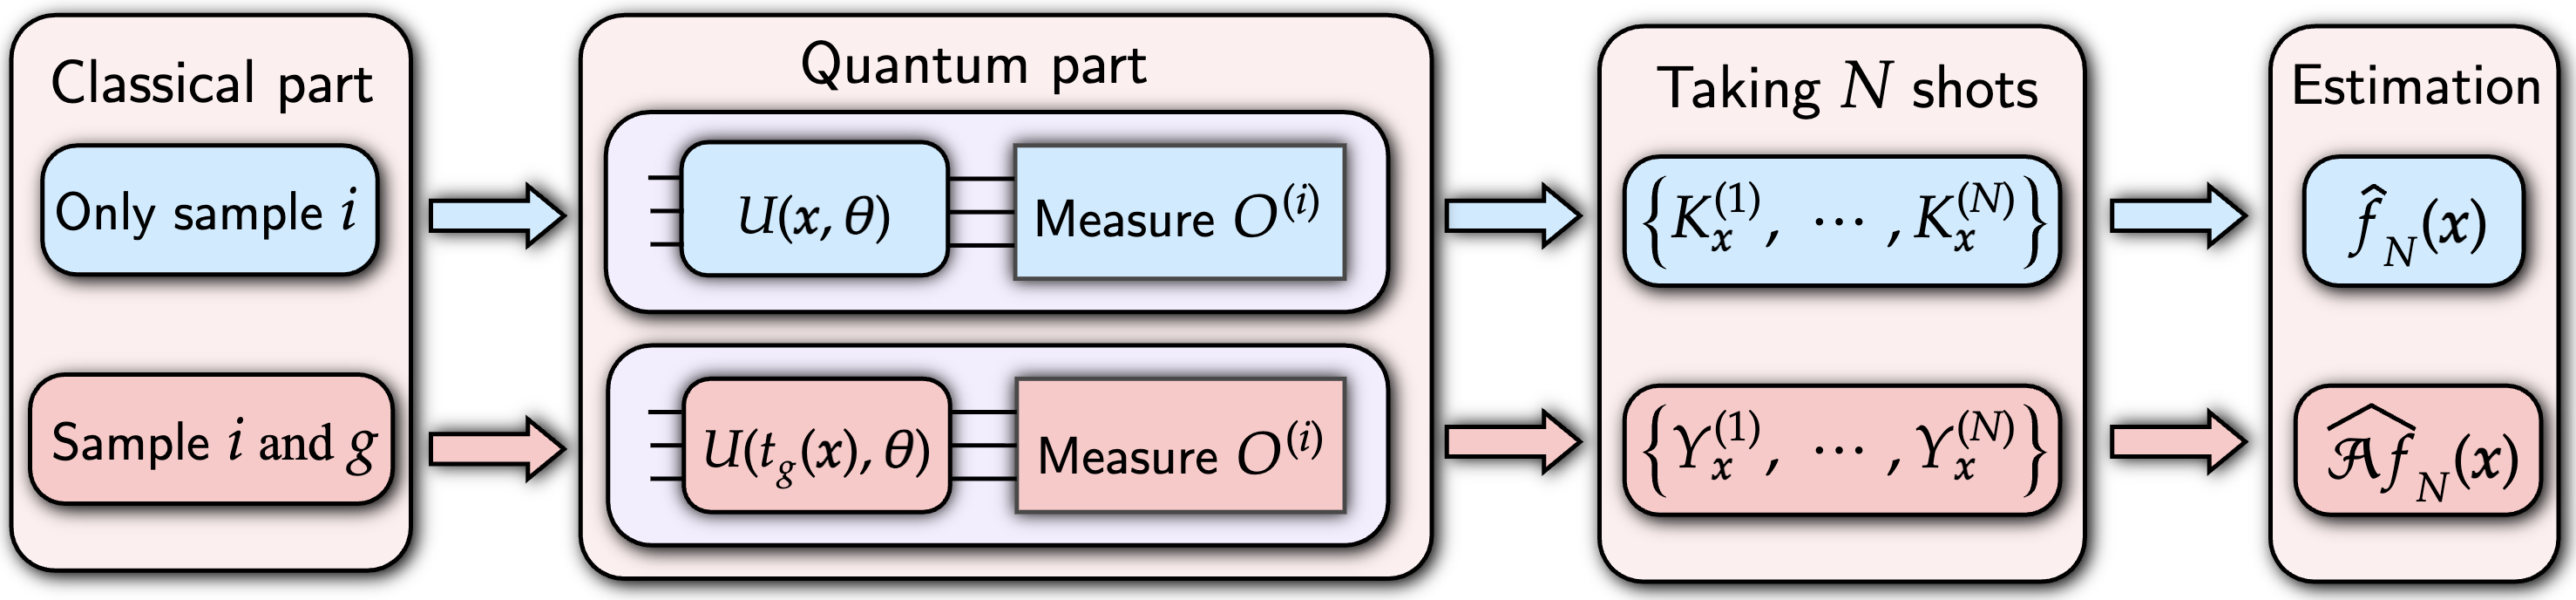
\includegraphics[width=0.9\linewidth]{figures/Workflow.png}
    \caption{Workflow of the randomized-encoding implementation of input-level symmetry averaging, shown in red, compared with the baseline model shown in blue. The quantum circuit architecture is unchanged; only the classical input supplied to the encoding layers is randomized.}
    \label{fig:workflow}
\end{figure*}

\subsection{Limitations of conventional methods}
\label{sec:limitation}

Lemma~\ref{lemma:invariance} gives a standard route to symmetry-invariant quantum models: one may combine an equivariant data embedding, equivariant trainable layers, an invariant initial state, and an invariant observable to obtain an invariant hypothesis function. This component-wise construction is powerful, but it also shifts the problem to the design of symmetry-compatible quantum objects. In particular, the symmetry of the classical data must first be represented on the Hilbert space, and the trainable part of the model must then be restricted to maps or gates that are equivariant with respect to this representation.

Several techniques have been developed to construct such equivariant objects, as summarized in Table~\ref{tab:resource_complexity}. The null-space and Choi-operator methods construct equivariant layers or channels by solving the corresponding representation-theoretic constraints. These methods are systematic, but their offline cost can scale exponentially with the number of qubits. Gate symmetrization instead starts from a standard gateset and projects its generators onto the commutant of the symmetry representation, thereby producing an equivariant gateset. This avoids solving for a full space of channels, but evaluating the group average can scale as \(\mathcal O(|\mathcal S|)\), and the resulting gates may be nonlocal or implementation dependent.

A different route is to implement the twirl directly at runtime. Deterministic twirling coherently realizes the group average using an ancilla register of size \(\lceil\log_2|\mathcal S|\rceil\) and controlled implementations of the group representation. Stochastic twirling removes the ancilla register by sampling a group element \(s\in\mathcal S\), but each sampled circuit still contains the representation circuit \(R(s)\) or \(R^\dagger(s)\). Hence, compared with the baseline circuit of depth \(D\), stochastic twirling incurs an additional quantum depth \(D_R\), as well as the corresponding gate-synthesis and hardware-control overhead. This makes stochastic twirling substantially more practical than coherent deterministic twirling, but it still implements symmetry through randomized representation circuits on the quantum device.

Randomized encoding uses a different randomized implementation. Instead of sampling \(s\) and appending the representation circuit \(R(s)\), it samples \(s\) and directly evaluates the transformed encoding layer
\[
E_s(x):=E(t_s(x)).
\]
Equivalently, the symmetry action is absorbed into the classical data supplied to the encoding circuit. Thus, both stochastic twirling and randomized encoding involve shot-wise or batch-wise randomized circuit instances, but the randomized component is different: stochastic twirling randomizes the representation circuit \(R(s)\), whereas randomized encoding randomizes the data-dependent encoding \(E_s(x)\). Since \(E_s(x)\) has the same circuit structure as the original encoding \(E(x)\), this replacement does not add the extra representation depth \(D_R\), does not require controlled symmetry operations, and leaves the trainable ansatz and observable unchanged. The advantage is therefore not the absence of randomization, but the fact that the randomized object is the encoding layer rather than an additional symmetry-representation circuit. The quantum circuit executed for each sampled \(s\) therefore uses the same number of qubits and the same depth \(D\) as the baseline model, while the additional sampling variance is analyzed separately in Sec.~\ref{sec:sampling_overhead}.


\section{Randomized-encoding implementation}
\label{sec:randomized_encoding}

We now describe how to implement the averaged predictor without explicitly applying a quantum group representation. The key observation is that, for data-encoding quantum models, the sampled symmetry transformation can often be applied to the classical input before encoding. Thus, instead of inserting a representation circuit \(R(s)\) into the quantum device, we evaluate the original circuit on a transformed input.

We first present the construction for a finite set of input transformations. Let \(\mathcal{G}\) be a finite set, and let \(t_g:\mathbb{R}^m\to\mathbb{R}^m\) denote the corresponding input transformation for \(g\in\mathcal{G}\). Given a probability distribution \(p(g)\) over \(\mathcal{G}\), we define the averaged predictor
\begin{equation}
\label{eq:average_op_def_pauli_stochastic}
(\mathcal{A}f)(\bm{x})
=
\sum_{g\in\mathcal{G}} p(g) f(t_g(\bm{x}))
=
\operatorname{Tr}\!\left(\hat{O}\bar{\rho}(\bm{x})\right),
\end{equation}
where
\begin{equation}
\bar{\rho}(\bm{x})
=
\sum_{g\in\mathcal{G}}p(g)\rho(t_g(\bm{x})).
\end{equation}
When \(\mathcal{G}\) is a symmetry group, \(t_g=V_g\), and \(p(g)=1/|\mathcal{G}|\), this reduces to the group-averaged predictor in Eq.~\eqref{eq:group_op_def} and is exactly invariant under the group action. More general choices of \(\mathcal{G}\) and \(p(g)\) can be used to define other input-averaged predictors, but exact group invariance is guaranteed only in the symmetry-averaging case.

The implementation of Eq.~\eqref{eq:average_op_def_pauli_stochastic} is straightforward in a shot-based quantum device. At each shot, one samples \(g\sim p\), replaces the input \(\bm{x}\) by \(t_g(\bm{x})\), and executes the same baseline circuit architecture \(U(t_g(\bm{x}),\bm{\theta})\). No additional quantum operation implementing the group representation is required.

Since estimating all \(M\) observables is computationally expensive, a common approach for efficient estimation is to sample the observable \(O^{(i)}\) randomly before each measurement, rather than iterating over all \(M\) Pauli strings \cite{Sweke2020,Andrew2020,Moussa_2023}. To formalize this, we introduce a probability distribution \(q(i)= |h_i| / \|h\|_1 > 0\) over the Pauli string indices \(i \in \{1, \dots, M\}\) and define a random variable \(I\) such that \(\mathbb{P}(I=i) = q(i)\).

\subsection{Randomized-encoding estimator}

Based on the above construction, we estimate the averaged predictor using the following randomized-encoding procedure, corresponding to the lower red branch in Fig.~\ref{fig:workflow}:

\begin{enumerate}
    \item \textbf{Classical randomization:} Sample an input transformation \(g\in\mathcal{G}\) according to \(p(g)\), and independently sample a Pauli-string index \(i\in\{1,\dots,M\}\) according to \(q(i)\).
    \item \textbf{Quantum evaluation:} Execute the baseline quantum circuit with the transformed input, \(U(t_g(\bm{x}),\bm{\theta})\), and measure the selected Pauli string \(O^{(i)}\). This gives a single-shot outcome \(z_{t_g(\bm{x})}^{(i)}\in\{-1,1\}\), which is a realization of \(Z_{t_g(\bm{x})}^{(i)}\).
    \item \textbf{Taking \(N\) shots:} Repeat the previous two steps \(N\) times. For the \(k\)-th shot, let \(g_k\), \(i_k\), and \(z_{t_{g_k}(\bm{x})}^{(i_k)}\) denote the sampled transformation, sampled Pauli string, and observed measurement outcome. Then
    \begin{equation}
    \frac{h_{i_k}}{q(i_k)}z_{t_{g_k}(\bm{x})}^{(i_k)}
    \end{equation}
    is one realization of the single-shot estimator \(Y_{\bm{x}}\).
    \item \textbf{Estimation:} Compute the empirical mean
    \begin{equation}
    \widehat{\mathcal{A}f}_N(\bm{x})
    :=
    \frac{1}{N}
    \sum_{k=1}^N
    \frac{h_{i_k}}{q(i_k)}
    z_{t_{g_k}(\bm{x})}^{(i_k)}
    \end{equation}
    as the randomized-encoding estimate of \((\mathcal{A}f)(\bm{x})\).
\end{enumerate}

Formally, \(Y_{\bm{x}}\) is a single-shot random variable such that the conditional random variable \((Y_{\bm{x}} \mid G=g, I=i)\) is distributed identically to \(\frac{h_i}{q(i)} Z_{t_g(\bm{x})}^{(i)}\). Since
\begin{equation}
\frac{h_i}{q(i)} Z_{t_g(\bm{x})}^{(i)}
= \left( \frac{h_i}{|h_i|} \right) \|h\|_1 Z_{t_g(\bm{x})}^{(i)},
\end{equation}
\(Y_{\bm{x}}\) is strictly bounded to the possible outcomes \(\pm\|h\|_1\). By the law of total expectation, we have
\begin{equation}
\begin{aligned}
\mathbb{E}\left[Y_{\bm{x}}\right]
&= \mathbb{E}_{G, I}\left[ \mathbb{E}\left[ Y_{\bm{x}} \mid G, I \right] \right] \\
&= \sum_{g \in \mathcal{G}} p(g) \sum_{i=1}^M q(i) \mathbb{E}\left[ \frac{h_i}{q(i)} Z_{t_g(\bm{x})}^{(i)} \mathrel{\Bigg|} G=g, I=i \right] \\
&= \sum_{g \in \mathcal{G}} p(g) \sum_{i=1}^M h_i \operatorname{Tr}(O^{(i)} \rho(t_g(\bm{x}))) \\
&= \operatorname{Tr}\left(\hat{O} \sum_{g \in \mathcal{G}} p(g) \rho(t_g(\bm{x}))\right) \\
&= \operatorname{Tr}(\hat{O} \bar{\rho}(\bm{x})) = (\mathcal{A} f)(\bm{x}).
\end{aligned}
\end{equation}
Since \(\{Y_{\bm{x}}^{(k)}\}_{k=1}^N\) is a set of independent and identically distributed random variables, where each \(Y_{\bm{x}}^{(k)}\) represents the outcome of the \(k\)-th shot and follows the same distribution as \(Y_{\bm{x}}\), we have
\begin{equation}
\widehat{\mathcal{A}f}_N(\bm{x}) = \frac{1}{N} \sum_{k=1}^N Y_{\bm{x}}^{(k)},
\qquad
\mathbb{E}\left[\widehat{\mathcal{A}f}_N(\bm{x})\right] = (\mathcal{A} f)(\bm{x}).
\end{equation}
Thus, the randomized-encoding estimator is an unbiased estimator for \((\mathcal{A} f)(\bm{x})\). By the central limit theorem, it follows the asymptotic Gaussian distribution
\begin{equation}
\widehat{\mathcal{A}f}_N(\bm{x})
\sim
\mathcal{N}\!\left((\mathcal{A}f)(\bm{x}), \frac{\operatorname{Var}(Y_{\bm{x}})}{N}\right)
\end{equation}
for sufficiently large \(N\). Precisely, with the Hoeffding bound for Pauli-decomposition observables presented in \cite{Gresch2025}, the following proposition establishes the sample complexity of this estimator.

\begin{proposition}
\label{prop:randomized_encoding_shots}
Let \(f: \mathcal{X} \to \mathbb{R}\) be a bounded function, and let \(\widehat{\mathcal{A}f}_N(\bm{x})\) be the randomized-encoding estimator for \((\mathcal{A} f)(\bm{x})\) defined in Eq.~\eqref{eq:average_op_def_pauli_stochastic}. The estimator guarantees an approximation error \(|(\mathcal{A} f)(\bm{x}) - \widehat{\mathcal{A}f}_N(\bm{x})| \leq \epsilon\) with probability at least \(1 - \delta\), provided that the number of samples \(N\) satisfies
\begin{equation}
N \geq \frac{2\|h\|_1^2}{\epsilon^2} \log \left(\frac{2}{\delta}\right),
\end{equation}
where \(\|h\|_1\) is the \(L_1\)-norm of the Pauli coefficients.
\end{proposition}

At first glance, evaluating \((\mathcal{A}f)(\bm{x})\) through randomized encoding appears to introduce an additional sampling overhead. However, if \(f(\bm{x})\) represents the hypothesis function of a quantum model, evaluating the original function already requires quantum measurements and shot-based sampling. Therefore, the more relevant question is whether evaluating the randomized-encoding averaged function requires a greater sample complexity than evaluating the original function \(f(\bm{x})\).

To formalize this comparison, consider the degenerate case as the \textit{baseline} model where \(t_g = \mathrm{id}\) for all \(g \in \mathcal{G}\), such that \(\bar{\rho}(\bm{x}) = \rho(\bm{x})\), which corresponds to the upper blue branch in Fig.~\ref{fig:workflow}. The hypothesis function of the baseline model is defined in Eq.~\eqref{eq:re-uploading_function}. Let \(K_{\bm{x}}\) denote the single-shot measurement outcome of the original function with expectation \(\mathbb{E}[K_{\bm{x}}] = f(\bm{x})\). The standard unbiased estimator \(\widehat{f}_N(\bm{x}) = \frac{1}{N} \sum_{k=1}^N K_{\bm{x}}^{(k)}\) follows the asymptotic distribution \(\mathcal{N}(f(\bm{x}), \operatorname{Var}(K_{\bm{x}})/N)\). Since both \(\widehat{\mathcal{A}f}_N\) and \(\widehat{f}_N\) are unbiased, the computational overhead of randomized encoding is restricted to the input transformations \(t_g\) and any increase in shot count. As established by concentration inequalities and asymptotic properties, the sample complexity is proportional to the variance of the single-shot random variable. Therefore, evaluating the overhead of randomized encoding reduces to a comparison between \(\operatorname{Var}(Y_{\bm{x}})\) and \(\operatorname{Var}(K_{\bm{x}})\), which we address in Sec.~\ref{sec:sampling_overhead}.

\subsection{Resource advantages}
\label{sec:randomized_encoding_advantage}

Twirling is currently one of the most practical and widely adopted methods for handling finite symmetry groups, making it highly relevant for near-term devices \cite{Nguyen2024,Cenk2024}. In this work, we primarily benchmark the randomized-encoding implementation against deterministic and stochastic twirling, with a particular focus on the latter.

We use the same resource convention as in Table~\ref{tab:resource_complexity}. Let \(D\) denote the circuit depth of one baseline evaluation \(U(\bm{x},\bm{\theta})\), and let \(D_R\) denote the compiled depth overhead required to implement the sampled symmetry representation associated with Eq.~\eqref{eq:eq_encoding} or Eq.~\eqref{eq:twirling}. If \(D_R\) is defined as the depth of a single \(R(s)\) block, then a twirling implementation of \(R(s)(\cdot)R(s)^\dagger\) contributes \(2D_R\); in Table~\ref{tab:resource_complexity} we absorb this constant factor into the definition of \(D_R\).

The key difference between stochastic twirling and randomized encoding is where the sampled symmetry is implemented. In stochastic twirling, each shot samples \(s\in\mathcal{S}\) and inserts a compiled symmetry-action block involving \(R(s)\), which increases the circuit depth from \(D\) to \(D+D_R\). In contrast, randomized encoding samples \(g\in\mathcal{G}\) and only replaces the classical input \(\bm{x}\) by \(t_g(\bm{x})\) inside the existing encoding layers \(E^{(l)}(\bm{x})\). Therefore, the quantum circuit architecture remains identical to the baseline circuit:
\begin{equation}
    \operatorname{depth}\!\left(U(t_g(\bm{x}),\bm{\theta})\right)
    =
    \operatorname{depth}\!\left(U(\bm{x},\bm{\theta})\right)
    =
    D,
\end{equation}
with \(D=\mathcal{O}(L)\) for a fixed-depth implementation of each re-uploading layer. Thus the additional quantum-depth overhead is
\begin{equation}
    \Delta D_{\mathrm{RE}}=0,
    \qquad
    \Delta D_{\mathrm{stoch}}=D_R,
    \qquad
    \Delta D_{\mathrm{det}}=\mathcal{O}(|\mathcal{S}|D_R).
\end{equation}
This is the resource sense in which randomized encoding avoids the cost of explicitly realizing the induced representation \(R(s)\).

% The magnitude of \(D_R\) is representation- and hardware-dependent. If \(R(s)\) is a local Pauli or phase operation, then \(D_R=\mathcal{O}(1)\) and no asymptotic quantum-resource advantage should be claimed. The advantage becomes substantial when \(R(s)\) is nonlocal under the device connectivity. For example, when \(R(s)\) is a qubit permutation on a linear-nearest-neighbor device, implementing a general permutation requires up to \(n(n-1)/2\) adjacent SWAP gates, i.e., up to \(3n(n-1)/2\) CNOT gates under the standard \(\mathrm{SWAP}=3\,\mathrm{CNOT}\) decomposition, and SWAP depth at most \(n\) \cite{Kutin2007}. For a uniformly sampled permutation in \(S_n\), the average number of adjacent SWAPs equals the average inversion number, \(n(n-1)/4\), yielding an average CNOT overhead \(3n(n-1)/4\) per sampled \(R(s)\). Similarly, for a uniformly sampled cyclic shift in \(C_n\), the average adjacent-SWAP count is \((n^2-1)/6\), yielding an average CNOT overhead \((n^2-1)/2\).

% Consequently, for nonlocal symmetry actions such as permutation symmetries on sparse-connectivity hardware, stochastic twirling incurs an additional \(\Theta(n)\) depth and \(\Theta(n^2)\) two-qubit-gate overhead per sampled symmetry action, whereas randomized encoding incurs no additional quantum gates beyond the baseline evaluation of \(U(t_g(\bm{x}),\bm{\theta})\). If one compares the entire randomized-encoding circuit to the standalone realization of \(R(s)\), then a sufficient condition for randomized encoding to be shallower is \(D<D_R\); for a shallow re-uploading architecture with \(D=\mathcal{O}(L)\) and permutation-type \(R(s)\) on a linear device, this holds whenever \(L=o(n)\).


\subsection{Sampling overhead}
\label{sec:sampling_overhead}

We now analyze how the variance of the randomized-encoding estimator \(Y_{\bm{x}}\) compares with the standard quantum measurement estimator \(K_{\bm{x}}\). Their variances are given by
\begin{align}
\operatorname{Var}\left[Y_{\bm{x}}\right]&=
\|h\|_1^2-((\mathcal{A}f)(\bm{x}))^2, \\
\operatorname{Var}[K_{\bm{x}}]&=
\|h\|_1^2-(f(\bm{x}))^2.
\end{align}
This immediately yields the following condition for variance reduction.

\begin{proposition}[Variance Reduction]
\label{prop:noise_down}
We have \(\operatorname{Var}(K_{\bm{x}}) > \operatorname{Var}(Y_{\bm{x}})\) if and only if
\begin{equation}
|(\mathcal{A}f)(\bm{x})| > |f(\bm{x})|.
\end{equation}
\end{proposition}

The proof is shown in Appendix~\ref{sec:variance_reduction}. Intuitively, this result can be understood by treating the single-shot estimators, \(K_{\bm{x}}\) and \(Y_{\bm{x}}\), as transformed Bernoulli distributions. Due to the sampling scheme, their outcomes are strictly limited to two symmetric values: \(\{+\|h\|_1, -\|h\|_1\}\). For such a distribution, the variance is determined entirely by its expectation. An expectation near zero means both outcomes are nearly equally likely, yielding maximum uncertainty, while a larger absolute expectation means the distribution is skewed toward one specific outcome. Therefore, the condition \(|(\mathcal{A}f)(\bm{x})| > |f(\bm{x})|\) means that the randomized-encoding estimator makes the measurement more predictable compared with the standard method. Consequently, fewer measurement shots are required to estimate the expectation value to a desired precision.

However, in many practical situations, applying the generalized average operator may instead increase the variance. Let \(\mathcal{X}\) denote the input domain and let \(h\) be an integrable function defined on \(\mathcal{X}\). We formally define a transformation \(t_g:\mathcal{X} \rightarrow \mathcal{X}\) as uniformity-preserving if it satisfies \(\int_{\mathcal{X}} h(t_g(\bm{x}))\,\mathrm{d}\bm{x} = \int_{\mathcal{X}} h(\bm{x})\,\mathrm{d}\bm{x}\) \cite{Basu2016}. Typical examples include permutations, translations, and rotations over \(\mathcal{X}\). Under such transformations, the additional input randomness can lead to inflation in the expected variance.

\begin{proposition}[Variance Inflation]
\label{prop:noise_up}
Consider \(t_g(\bm{x})\) as uniformity-preserving transformations for all \(g\in\mathcal{G}\). Then
\begin{equation}
\mathbb{E}\left[\operatorname{Var}\left[K_{\bm{x}}\right]\right] \leq \mathbb{E}\left[\operatorname{Var}\left[Y_{\bm{x}}\right]\right] \leq  \|h\|_1^2,
\end{equation}
where the expectation \(\mathbb{E}[\cdot]\) is taken over \(\bm{x}\) drawn uniformly from \(\mathcal{X}\).
\end{proposition}

The proof is shown in Appendix~\ref{sec:variance_inflation}. Under these conditions, the randomized-encoding estimator is noisier on average than the standard estimator, reflecting the shot overhead introduced by input randomization.

While input-level randomization can increase the number of shots required to reach a target accuracy \(\epsilon\), this cost remains bounded. Bernstein's inequality defines the shot count as \(N \geq \left(2 \sigma \varepsilon^{-2}+\frac{4\|h\|_1}{3}\varepsilon^{-1}\right) \ln( 2\delta^{-1})\), where \(\sigma\) is the estimator variance, e.g., \(\operatorname{Var}(Y_x)\) or \(\operatorname{Var}(K_x)\). However, Proposition~\ref{prop:noise_up} ensures that this variance is strictly bounded by \(\|h\|_1^2\), meaning that expanding the transformation set \(\mathcal{G}\) does not trigger an indefinite growth in sampling cost. In fact, the Hoeffding bound \(N \geq \frac{2}{\epsilon^2}\|h\|_1^2 \log \frac{2}{\delta}\) \cite{Gresch2025} is invariant to the randomness introduced by randomized encoding. Together, these results show that the statistical price of randomized encoding is controlled, while the quantum circuit depth and qubit count remain those of the baseline model.

\subsection{Physical implementation}

In our framework, each measurement shot requires updating the input to \(t_g(\bm{x})\) according to a sampled index \(g \in G\). To preserve the resource advantage of randomized encoding, the input update rate must be comparable to, or faster than, the measurement shot rate. This requirement is challenging for several quantum computing platforms. For instance, in trapped-ion systems, input parameters are typically implemented via precisely timed laser pulse sequences within a relatively slow experimental cycle. Although programmable, this control paradigm does not naturally support fast shot-wise parameter updates, making such randomized input schemes challenging to realize in practice.

A more suitable platform is continuous-variable photonic quantum computing. In such implementations, input-dependent unitaries \(U(\bm{x})\) are realized via electro-optic modulation, where parameters such as phase shifts and displacements are directly controlled by applied voltages. Consequently, transformations \(t_g(\bm{x})\) can be implemented by modifying classical electrical signals, without altering the underlying optical circuit.

Importantly, modern electro-optic modulators support bandwidths ranging from MHz to GHz, which can exceed typical photonic measurement repetition rates. This allows parameter updates to be performed at the shot level with negligible overhead, making randomized input transformations effectively hardware-efficient in these platforms.

Prior photonic experiments already implement shot-dependent randomization of the input configuration, where heralded photons are injected shot by shot into different random input ports of an interferometer \cite{Marco2015}. Related work has also proposed efficient readout error mitigation schemes based on approximate-state measurements, applying randomly drawn unitary rotations on each qubit immediately prior to measurement \cite{Andrew2023}. In addition, measurement directions set by phases can be reset reproducibly on each repetition, so varying the phase across repetitions can in principle enable shot-by-shot changes of the measurement direction \cite{Ding2024}. Indefinite-outcome circuit protocols enable shot-by-shot online calibration by updating control parameters after each measurement outcome, supported by low-latency FPGA-based controllers \cite{Alicia2025}. Recent work on low-latency FPGA/cryo-CMOS control has shown that shot-to-shot updates of control parameters are compatible with contemporary quantum control architectures, supporting the hardware plausibility of per-shot adaptive or randomized circuit reconfiguration \cite{Miller2025}.

A recent trapped-ion study showed that applying augmentations directly in the classical input space before quantum encoding can improve downstream QML performance, supporting the broader idea that classical input transformations provide an effective way to inject inductive bias into quantum models \cite{Liudmila2025}.

\section{Numerical experiments}
\label{sec:experiment}

\subsection{1-Qubit QPINN for ODE Solving}

We demonstrate the efficacy of our approach by solving the driven damped harmonic oscillator equation using a 1-qubit quantum physics-informed neural network. The target ordinary differential equation is
\begin{equation}
     \frac{\partial^2 f(x)}{\partial x^2}+ \frac{\partial f(x)}{\partial x} + f(x)  = \sin(x),
\end{equation}
which has the exact solution \(f(x) = -\cos(x)\). To approximate this solution, we employ a data re-uploading quantum ansatz defined by the parameterized unitary
\begin{equation}
U(x, \bm{\theta}) = R_x(\theta_0) R_z(\theta_1) R_y(x).
\end{equation}
Measuring the observable \(O = Z\), this specific 1-qubit ansatz expands analytically to
\begin{equation}
f(x, \bm{\theta}) = \cos(\theta_0)\cos(x) + \sin(\theta_0)\sin(\theta_1)\sin(x).
\end{equation}
The model is trained by minimizing the mean squared error loss of the ODE residual over \(N\) points,
\begin{equation}
\mathcal{L}(\bm{\theta}) = \frac{1}{2N} \sum_{i=1}^{N} r(x_i, \bm{\theta})^2,
\end{equation}
where \(r(x, \bm{\theta}) = \partial_x^2 f + \partial_x f + f - \sin(x)\). Parameter optimization is governed by the full gradient expression
\begin{align}
 \frac{\partial \mathcal{L}(\bm{\theta})}{\partial \theta_k} &= \frac{1}{N} \sum_{i=1}^{N} \left( \frac{\partial^2 f}{\partial x^2} + \frac{\partial f}{\partial x} + f - \sin(x_i) \right) \\
&\quad\times \left( \frac{\partial^3 f}{\partial x^2 \partial \theta_k} + \frac{\partial^2 f}{\partial x \partial \theta_k} + \frac{\partial f}{\partial \theta_k} \right).
\end{align}

\begin{figure}[t]
    \centering
    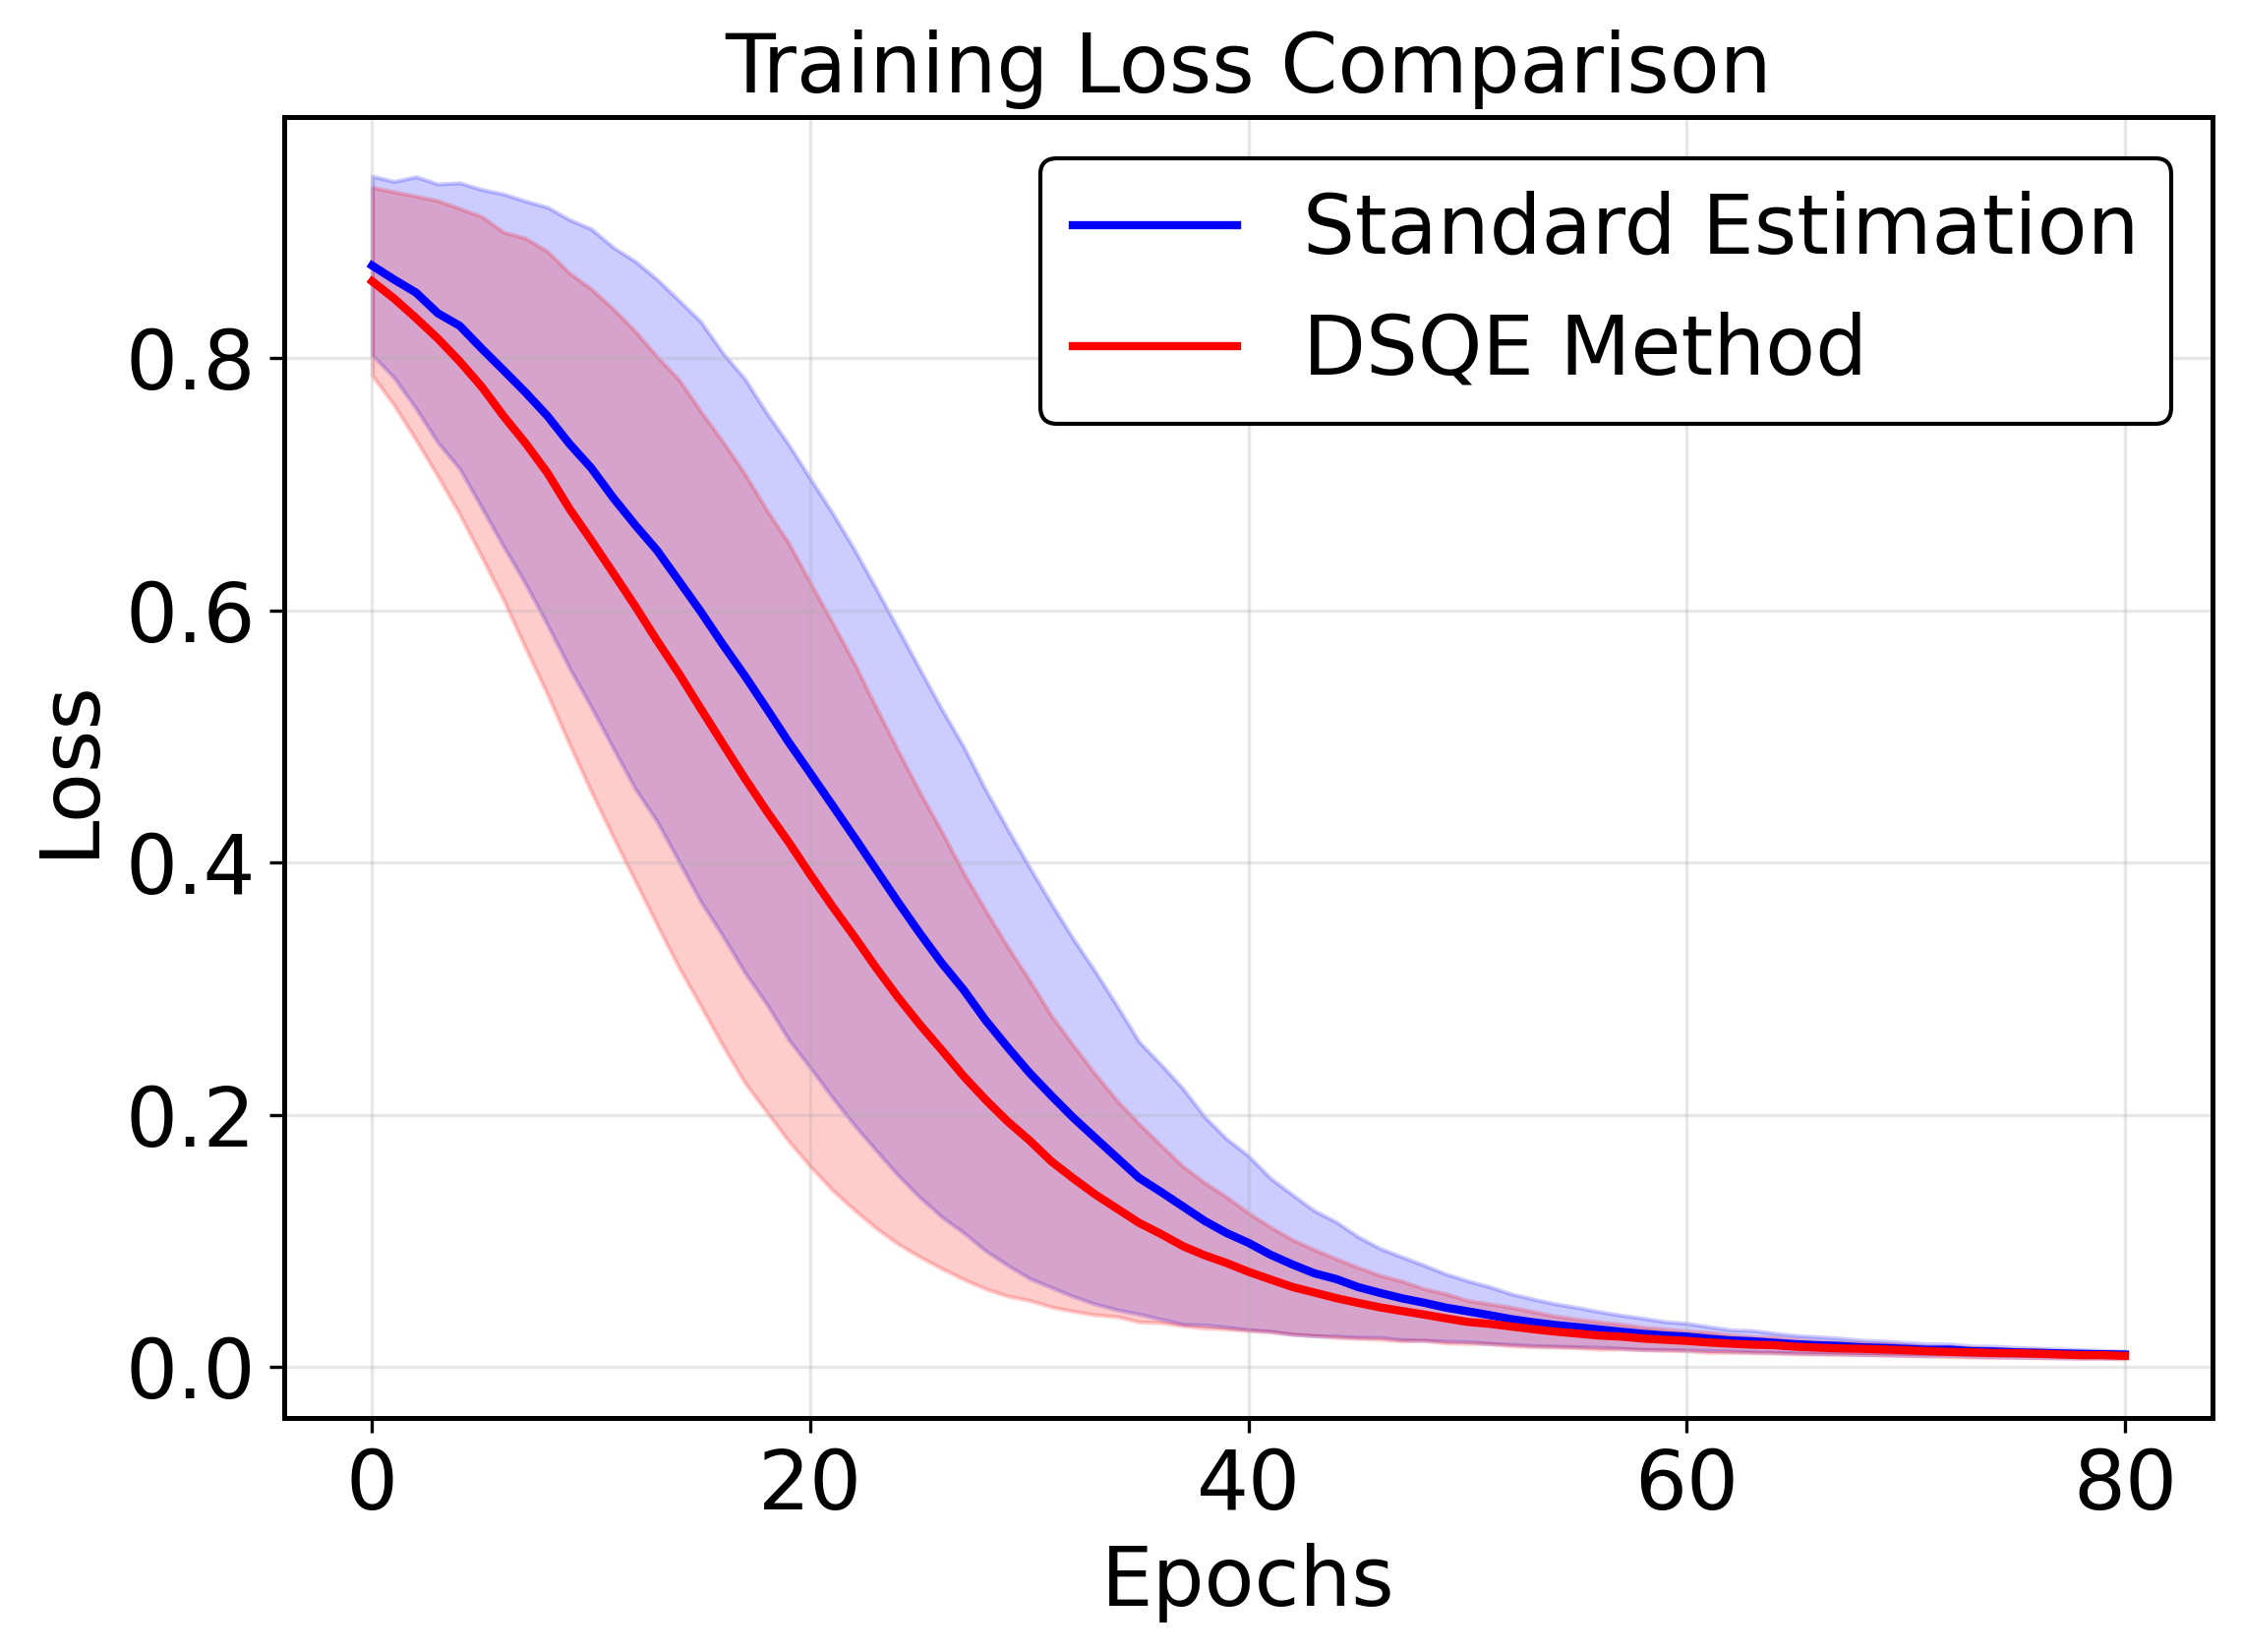
\includegraphics[width=\columnwidth]{figures/ODE_loss.png}
    \caption{Loss comparison for the ODE solver.}
    \label{fig:ODE_loss}
\end{figure}

\subsection{Boundary-Constrained QPINNs for a Screened Poisson Equation}

We further evaluate the proposed symmetry-induced hypothesis space on a two-dimensional physics-informed learning problem with explicit boundary constraints. The physical domain is the square \(\Omega=(-1,1)^2\), and the target field \(u:\bar{\Omega}\rightarrow\mathbb{R}\) solves the screened Poisson equation
\begin{equation}
    -\frac{\partial^2 u}{\partial x_1^2}(x_1,x_2)
    -\frac{\partial^2 u}{\partial x_2^2}(x_1,x_2)
    +\lambda u(x_1,x_2)
    = q(x_1,x_2),
    \qquad (x_1,x_2)\in\Omega,
\end{equation}
with homogeneous Dirichlet boundary condition
\begin{equation}
    u(x_1,x_2)=0,\qquad (x_1,x_2)\in\partial\Omega.
\end{equation}
In all experiments we set \(\lambda=1\). To obtain a controlled benchmark with a known solution, define
\begin{equation}
    \phi_m(t)=\cos\left(\frac{m\pi t}{2}\right),
\end{equation}
and choose the source term
\begin{equation}
    q(x_1,x_2)=\phi_1(x_1)\phi_1(x_2)
    +0.3\left[\phi_1(x_1)\phi_3(x_2)+\phi_3(x_1)\phi_1(x_2)\right].
\end{equation}
The corresponding analytical solution is
\begin{equation}
    u_\star(x_1,x_2)=
    \frac{\phi_1(x_1)\phi_1(x_2)}{\lambda+\pi^2/2}
    +\frac{0.3\left[\phi_1(x_1)\phi_3(x_2)+\phi_3(x_1)\phi_1(x_2)\right]}{\lambda+5\pi^2/2}.
    \label{eq:screened_poisson_exact_solution}
\end{equation}
This solution satisfies the boundary condition because \(\phi_1(\pm 1)=\phi_3(\pm 1)=0\), and each product mode is an eigenfunction of \(-\Delta+\lambda\).

For a model prediction \(u_\theta\), the interior residual is
\begin{equation}
    r_\theta(x_1,x_2)=
    -\frac{\partial^2 u_\theta}{\partial x_1^2}(x_1,x_2)
    -\frac{\partial^2 u_\theta}{\partial x_2^2}(x_1,x_2)
    +\lambda u_\theta(x_1,x_2)
    -q(x_1,x_2),
\end{equation}
where all derivatives are evaluated by automatic differentiation. We compare hard and soft treatments of the Dirichlet constraint. In the hard-constrained case, the final ansatz is
\begin{equation}
    u_\theta(x_1,x_2)=B(x_1,x_2)v_\theta(x_1,x_2),
    \qquad
    B(x_1,x_2)=\cos\left(\frac{\pi x_1}{2}\right)\cos\left(\frac{\pi x_2}{2}\right),
\end{equation}
so \(u_\theta=0\) on \(\partial\Omega\) for every parameter value and the optimized objective is the residual loss
\begin{equation}
    \mathcal{L}_{\mathrm{hard}}(\theta)
    =\frac{1}{N_\Omega}\sum_{i=1}^{N_\Omega} r_\theta(x_i)^2.
\end{equation}
In the soft-constrained case, the model directly outputs \(u_\theta=v_\theta\) and the boundary condition is imposed through a penalty,
\begin{equation}
    \mathcal{L}_{\mathrm{soft}}(\theta)
    =\frac{1}{N_\Omega}\sum_{i=1}^{N_\Omega} r_\theta(x_i)^2
    +\gamma\frac{1}{N_{\partial\Omega}}\sum_{j=1}^{N_{\partial\Omega}}u_\theta(y_j)^2,
    \qquad \gamma=10.
\end{equation}

The quantum models use the same two-qubit data re-uploading circuit: two upload layers, two strongly entangling layers per trainable block, \(R_X(\beta_j z_j)\) encoding gates with \(\beta_j=3^j\), and a final local projector observable averaged over the two qubits. This gives \(36\) trainable circuit parameters for each QPINN. We test three QPINN hypothesis spaces: (i) a Fourier-QPINN \(v_\theta(\bm{x})=f_\theta(\bm{x})\), (ii) a Chebyshev-QPINN \(v_\theta(\bm{x})=f_\theta(\arccos\bm{x})\), where \(\arccos\) is applied componentwise, and (iii) a \(B_2\)-QPINN
\begin{equation}
    v_\theta(\bm{x})
    =\frac{1}{|B_2|}\sum_{g\in B_2} f_\theta(g\bm{x}),
\end{equation}
which exactly averages over the two-dimensional hyperoctahedral group generated by coordinate sign flips and permutations. This deterministic average isolates the modeling effect of the \(B_2\) symmetry prior before replacing it by the randomized-encoding estimator discussed above. As a classical baseline, we also train a fully connected PINN with two hidden layers of width \(8\), \(\tanh\) activations, and \(105\) trainable parameters.

All models are trained with Adam for \(300\) steps over \(10\) independent initializations. Each step uses \(50\) interior collocation points sampled uniformly from \([-0.94,0.94]^2\) and \(50\) boundary points sampled uniformly over the four edges. The learning rate starts from \(10^{-1}\), decays by a factor \(0.99\) after each step, is lower bounded by \(10^{-4}\), and gradients are clipped at norm \(5\). The plots report geometric mean training curves over the \(10\) runs with one geometric standard deviation as the shaded band, and solution errors are evaluated as relative \(L^2\) errors on a \(41\times 41\) grid.

\begin{figure*}[t]
    \centering
    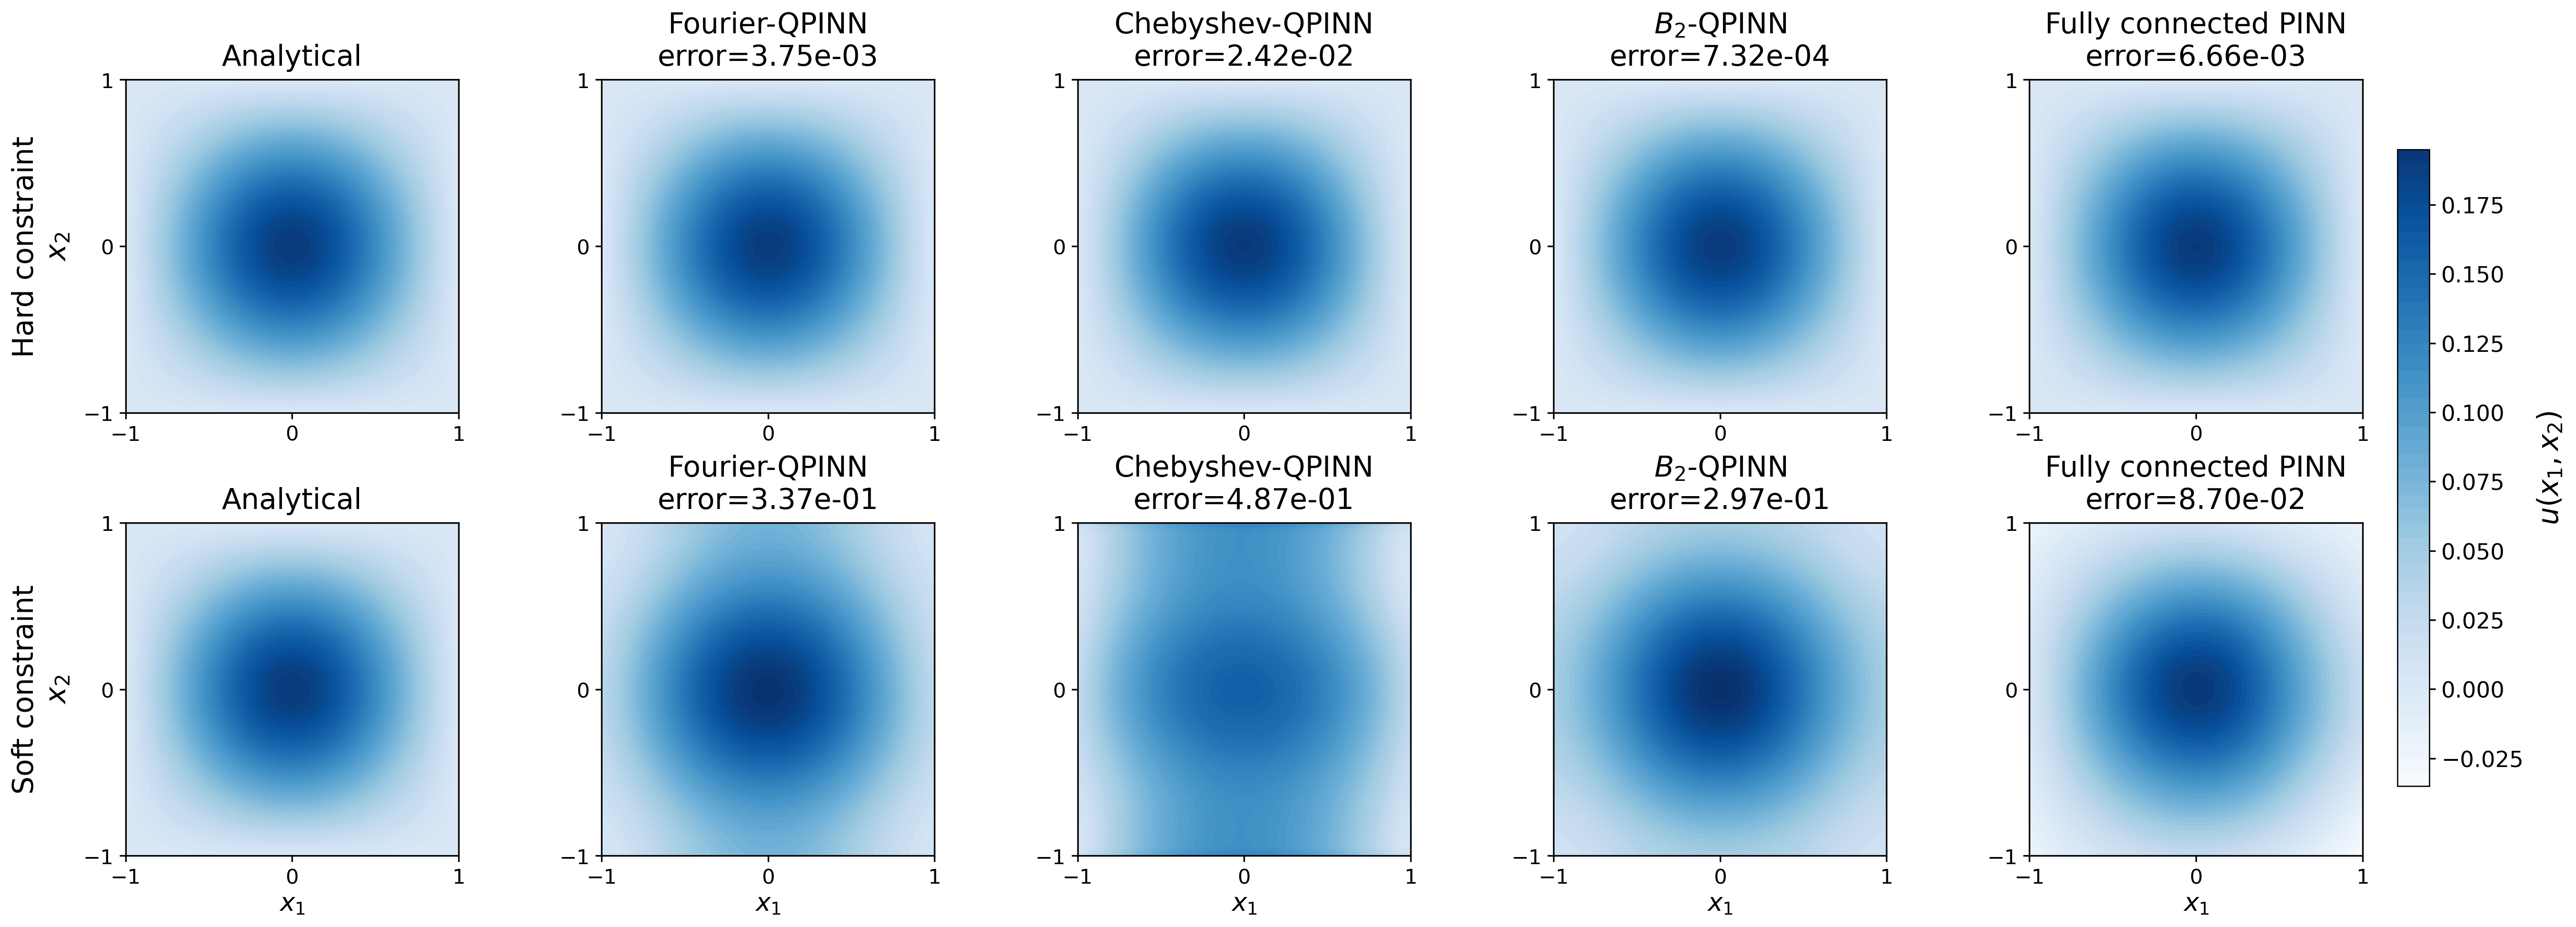
\includegraphics[width=0.98\textwidth]{figures/qpinn_boundary_constraint_solution_comparison_combined.png}
    \caption{Solution comparison for the screened Poisson benchmark. Rows correspond to hard and soft enforcement of the homogeneous Dirichlet boundary condition, while columns show the analytical solution, the three QPINN models, and the fully connected PINN baseline. Panel titles report the relative \(L^2\) error of the representative run selected by the lowest final training objective for the corresponding constraint formulation.}
    \label{fig:qpinn_boundary_constraint_solution}
\end{figure*}

\begin{figure*}[t]
    \centering
    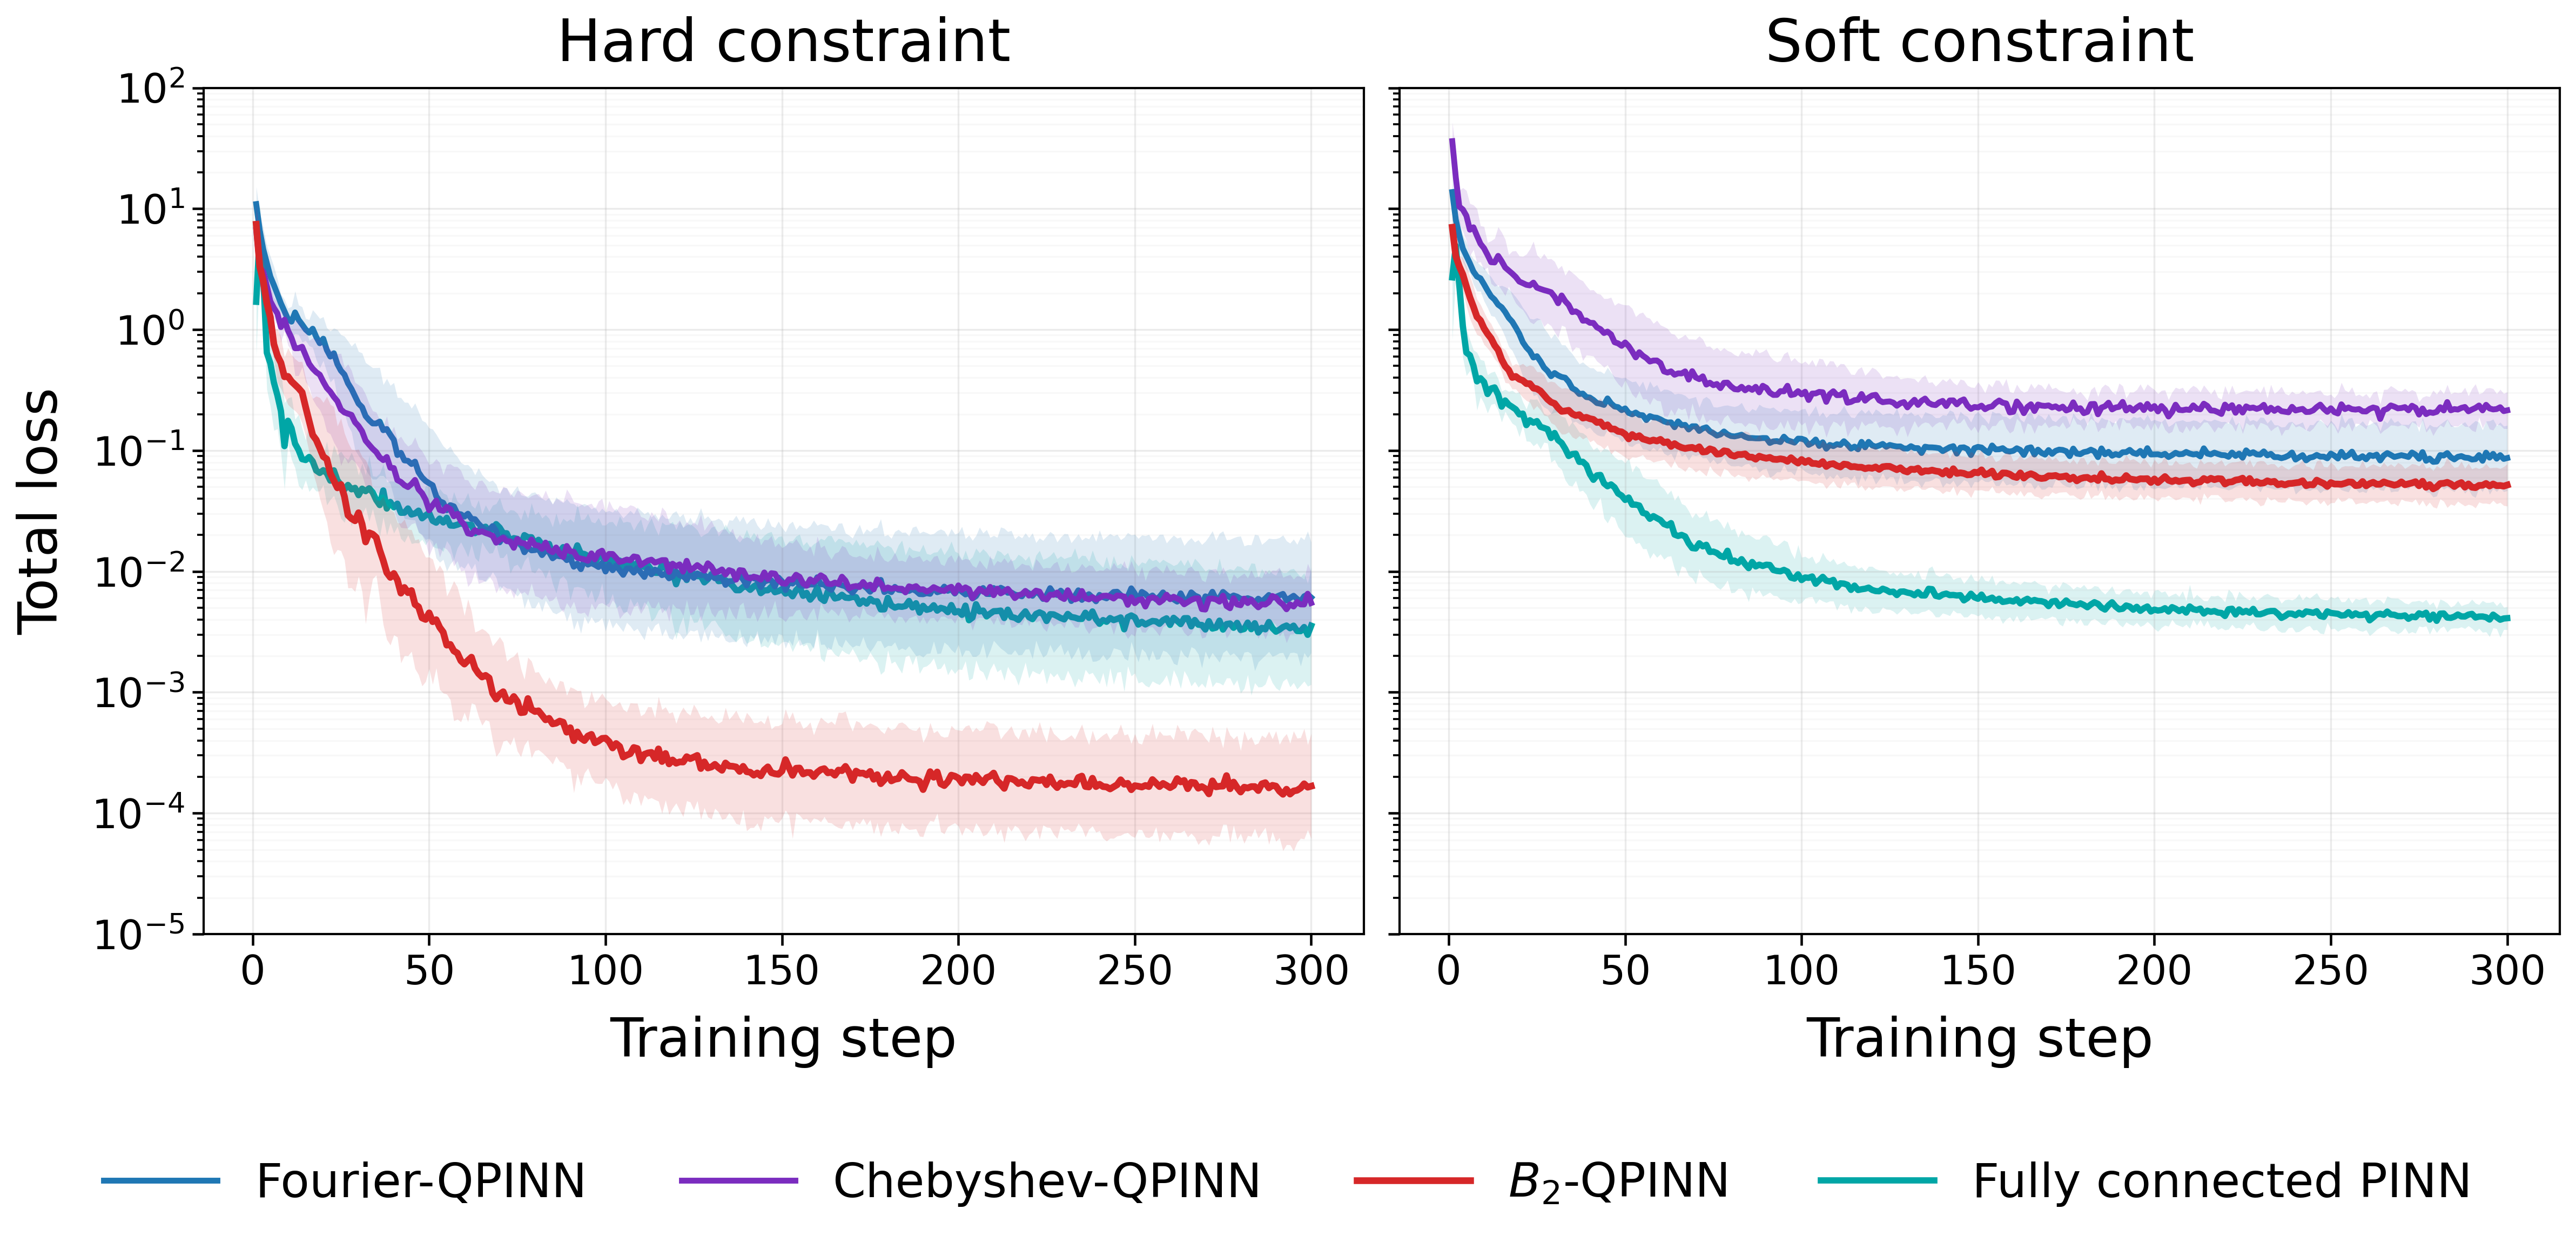
\includegraphics[width=0.98\textwidth]{figures/qpinn_boundary_constraint_loss_comparison_side_by_side.png}
    \caption{Hard- and soft-constraint training dynamics for the screened Poisson benchmark. In the hard case, the plotted objective is the residual loss because the boundary condition is satisfied by construction; in the soft case, the plotted objective includes the boundary penalty with weight \(\gamma=10\). Curves show geometric means over \(10\) independent runs, and shaded regions denote one geometric standard deviation.}
    \label{fig:qpinn_boundary_constraint_loss}
\end{figure*}

\section{Conclusion}

We have studied an input-level implementation of symmetry averaging for data-encoding quantum machine learning models. Rather than introducing a new stochastic averaging principle, our main observation is that, when the symmetry acts on the classical input before quantum encoding, the group-averaged predictor can be estimated by randomized encoding. This avoids the need to implement the corresponding quantum representation \(R(s)\) on hardware and therefore removes the associated representation-circuit depth, routing, and qubit overhead.

The resulting estimator is unbiased for the averaged predictor and requires the same quantum circuit architecture as the baseline model. Its cost is instead statistical: input-level randomization can change the single-shot variance and hence the number of shots required to reach a target precision. We derived this variance explicitly and showed that the shot overhead is bounded by the same \(\|h\|_1\)-dependent concentration bounds that govern standard Pauli-sampling estimators.

Beyond the estimator itself, we analyzed the Fourier structure induced by symmetry averaging in quantum Fourier models. The averaging operation groups Fourier modes into symmetry orbits and aggregates their coefficients, which can mitigate vanishing expressivity when the relevant orbit sizes are sufficiently large. We also showed that sign-flip averaging yields quantum Chebyshev models, providing a symmetry-based route to pure Chebyshev polynomial hypothesis spaces for quantum physics-informed learning.

These results position randomized encoding as a resource-efficient alternative to representation-level twirling in settings where the symmetry acts naturally on classical input data. It does not replace general equivariant quantum architectures, which remain necessary for symmetries intrinsic to quantum states or channels. Rather, it identifies an important practical regime in which symmetry enforcement can be moved from the quantum circuit to classical shot-wise input control.

\begin{acknowledgments}
\end{acknowledgments}

\bibliography{apssamp}

\clearpage
\onecolumngrid
\appendix

\section{GQML}
\label{sec:invariance}

\begin{restate}{Lemma}{lemma:invariance}
A data re-uploading quantum model defined in Eq.~\eqref{eq:re-uploading_function} induces an \(\mathcal{S}\)-invariant hypothesis function if it satisfies four conditions with respect to a symmetry group \(\mathcal{S}\): equivariant encoding and trainable layers, and an invariant initial state and observable.
\end{restate}

\begin{proof}
To prove that the hypothesis function \(f(\bm{x}, \bm{\theta})\) is \(\mathcal{S}\)-invariant, we must show that \(f(V_s[\bm{x}], \bm{\theta}) = f(\bm{x}, \bm{\theta})\) for all \(s \in \mathcal{S}\). We begin by formalizing the four given requirements using a unitary induced representation \(R(s)\):
\begin{enumerate}
    \item \textbf{Equivariant encoding layer:}
    \begin{equation}
    E^{(l)}(V_s[\bm{x}]) = R(s) E^{(l)}(\bm{x}) R(s)^\dagger \quad \forall s \in \mathcal{S}.
    \end{equation}
    \item \textbf{Equivariant trainable layers:} The parameterized layers commute with the induced representation:
    \begin{equation}
    [W^{(l)}(\bm{\theta}), R(s)] = 0 \implies W^{(l)}(\bm{\theta}) = R(s) W^{(l)}(\bm{\theta}) R(s)^\dagger.
    \end{equation}
    \item \textbf{Invariant initial state:}
    \begin{equation}
    R(s)|0\rangle\langle0|R(s)^\dagger = |0\rangle\langle0|.
    \end{equation}
    \item \textbf{Invariant observable:}
    \begin{equation}
    R(s)^\dagger \hat{O} R(s) = \hat{O}.
    \end{equation}
\end{enumerate}
First, we expand the unitary evolution \(U(V_s[\bm{x}], \bm{\theta})\) for a symmetrically transformed input \(V_s[\bm{x}]\). By applying conditions (1) and (2), adjacent \(R(s)^\dagger\) and \(R(s)\) terms cancel, so the entire parameterized circuit transforms equivariantly:
\begin{equation}
\begin{aligned}
U(V_s[\bm{x}], \bm{\theta})
&= R(s) U(\bm{x}, \bm{\theta}) R(s)^\dagger.
\end{aligned}
\end{equation}
Next, applying this unitary equivariance together with the invariant initial state condition gives
\begin{equation}
\begin{aligned}
\rho(V_s[\bm{x}], \bm{\theta})
&= U(V_s[\bm{x}], \bm{\theta}) |0\rangle\langle0| U^\dagger(V_s[\bm{x}], \bm{\theta}) \\
&= R(s) U(\bm{x}, \bm{\theta}) |0\rangle\langle0| U^\dagger(\bm{x}, \bm{\theta}) R(s)^\dagger \\
&= R(s) \rho(\bm{x}, \bm{\theta}) R(s)^\dagger.
\end{aligned}
\end{equation}
Finally, using the cyclic property of the trace and the invariant observable condition, we obtain
\begin{equation}
\begin{aligned}
f(V_s[\bm{x}], \bm{\theta})
&= \operatorname{Tr}\left(\hat{O}\rho(V_s[\bm{x}], \bm{\theta})\right) \\
&= \operatorname{Tr}\left(\hat{O}R(s)\rho(\bm{x}, \bm{\theta})R(s)^\dagger\right) \\
&= \operatorname{Tr}\left(R(s)^\dagger \hat{O} R(s)\rho(\bm{x}, \bm{\theta})\right) \\
&= \operatorname{Tr}\left(\hat{O}\rho(\bm{x}, \bm{\theta})\right) \\
&= f(\bm{x}, \bm{\theta}).
\end{aligned}
\end{equation}
This concludes the proof that the model induces an \(\mathcal{S}\)-invariant hypothesis function.
\end{proof}

\section{Fourier representation of re-uploading models}

Without loss of generality, we consider a parameter vector \(\bm{x}=(x_1,\dots,x_D)\) and \(L\) encoding layers each of the form
\[
S^{(l)}(\bm{x})
\;=\;
\bigotimes_{i=1}^D e^{-i\,x_i\,H_l^i},
\qquad l=1,\dots,L,
\]
where each \(H_l^i\) has eigenvector \(\{\lvert j_i^l\rangle\}_{j_i^l=1}^d\) with \(\;H_l^i\lvert j_i^l\rangle=\lambda_{j_i^l}\lvert j_i^l\rangle\), write
\[
j^l=(j^l_1,\dots,j^l_D)\in[1,d]^D,|j^l\rangle=|j^l_1\rangle \otimes\dots  \otimes|j^l_D\rangle
\]
Then
\[
S^{(l)}(\bm{x})\lvert j^l\rangle=\bigotimes_{i=1}^D e^{-i\,x_i\,H_l^i}|j^l_i\rangle
=\bigotimes_{i=1}^D e^{-i\,x_i\,\lambda_{j_i^l}}|j^l_i\rangle
=e^{-i\sum_{i=1}^D x_i\,\lambda_{j_i^l}}\lvert j^l\rangle.
\]
Using the identity $I=\sum_{j^1\in[1,d]^D}\lvert j^1\rangle\langle j^1\rvert$, consider $\lvert0\rangle=\lvert j^0\rangle$, we insert before \(W^{(1)}\):
\[
W^{(1)}\lvert0\rangle
=I\,W^{(1)}\lvert0\rangle
=\sum_{j^1\in[1,d]^D}\lvert j^1\rangle\langle j^1\rvert W^{(1)}\lvert j^0\rangle.
\]
Define $W^{(1)}_{\,j^1,j^0}
=\langle j^1\rvert W^{(1)}\lvert j^0\rangle$, so that
\[
W^{(1)}\lvert0\rangle
=\sum_{j^1\in[1,d]^D}W^{(1)}_{\,j^1,j^0}\,\lvert j^1\rangle.
\]
Applying the first encoding layer:
\[
S^{(1)}(\bm{x})\,W^{(1)}\lvert0\rangle
=\sum_{j^1\in[1,d]^D}W^{(1)}_{\,j^1,j^0}
\,e^{-i\sum_{i}^Dx_i\,\lambda_{j^1_i}}
\lvert j^1\rangle.
\]
Then the second layer:
\[
\begin{aligned}
&S^{(2)}(\bm{x})\,W^{(2)}\,S^{(1)}(\bm{x})\,W^{(1)}\lvert0\rangle\\
&= S^{(2)}(\bm{x})
  \Bigl(\sum_{j^2\in[1,d]^D}\ket{j^2}\bra{j^2}\Bigr) W^{(2)}
  \sum_{j^1\in[1,d]^D}
  W^{(1)}_{\,j^1,j^0}\,
  e^{-i\sum_{i=1}^D x_i\,\lambda_{j^1_i}}
  \,\ket{j^1}.\\
&=\sum_{j^2,j^1\in[1,d]^D}
\bra{j^2}W^{(2)}\ket{j^1}\,
  W^{(1)}_{\,j^1,j^0}\,
  e^{-i\sum_{i=1}^D x_i\,\lambda_{j^1_i}}
  \;S^{(2)}(\bm{x})\ket{j^2}\\
&=\sum_{j^2,j^1\in[1,d]^D}
  W^{(2)}_{\,j^2,j^1}\,
  W^{(1)}_{\,j^1,j^0}\,
  e^{-i\sum_{i=1}^D x_i\,\lambda_{j^1_i}}\,
  e^{-i\sum_{i=1}^D x_i\,\lambda_{j^2_i}}\,
  \ket{j^2}
\end{aligned}
\]
and so on. After \(L\) layers:
\[
\prod_{l=1}^L S^{(l)}(\bm{x})\,W^{(l)}\lvert0\rangle
=\sum_{j^L,\dots,j^1\in[1,d]^D}
\biggl[\prod_{l=1}^L W^{(l)}_{\,j^l,j^{l-1}}
e^{-i\sum_{i=1}^D x_i\,\lambda_{j_i^l}}\biggr]
\lvert j^L\rangle.
\]
Define the total path \(J=(j^1,\dots,j^L)\in[1,d]^{DL}\) , $|j^l\rangle$ is the eigenvector of  $\bigotimes_{i=1}^D H_l^i$,
\[
\boldsymbol\Lambda_J
=\bigl(\Lambda_J^1,\dots,\Lambda_J^D\bigr),
\quad
\Lambda_J^i=\sum_{l=1}^L\lambda_{j_i^l}.
\]
then
$$
\begin{aligned}
&\sum_{j^L,\dots,j^1\in[1,d]^D}
\biggl[(\prod_{l=1}^L W^{(l)}_{\,j^l,j^{l-1}})
e^{-i\sum_{i=1}^D x_i\,\lambda_{j^1_i}-\ldots-i\sum_{i=1}^D x_i\,\lambda_{j_i^l}}
\biggr]
\lvert j^L\rangle\\
&=\sum_{j^L,\dots,j^1\in[1,d]^D}
\biggl[(\prod_{l=1}^L W^{(l)}_{\,j^l,j^{l-1}})
e^{-i\sum_{i=1}^D x_i(\lambda_{j^1_i}+\ldots+\lambda_{j_i^l})}
\biggr]
\lvert j^L\rangle\\
&=\sum_{j^L,\dots,j^1\in[1,d]^D}
\biggl[(\prod_{l=1}^L W^{(l)}_{\,j^l,j^{l-1}})
e^{-i\sum_{i=1}^D x_i\Lambda_J^i}
\biggr]
\lvert j^L\rangle\\
\end{aligned}
$$
So
\[
\prod_{l=1}^L S^{(l)}(\bm{x})\,W^{(l)}\lvert0\rangle
=\sum_{j^L,\dots,j^1\in[1,d]^D}
\Bigl(\prod_{l=1}^L W^{(l)}_{\,j^l,j^{l-1}}\Bigr)\,
e^{-i\,\bm{x}\cdot\boldsymbol\Lambda_J}\,
\lvert j^L\rangle.
\]
After \(L\) layers the state is
\[
\ket{\psi_L(\bm{x})}
=\sum_{J}
\Bigl(\prod_{l=1}^L W^{(l)}_{\,j^l,j^{l-1}}\Bigr)
e^{-i\,\bm{x}\cdot\boldsymbol\Lambda_J}
\;\ket{j^L}.
\]
Applying the final trainable layer \(W^{(L+1)}\) gives
\[
U(\bm{x},\bm{\theta})\ket{0}
=W^{(L+1)}\ket{\psi_L(\bm{x})}
=\sum_{J}
\Bigl(\prod_{l=1}^L W^{(l)}_{\,j^l,j^{l-1}}\Bigr)
e^{-i\,\bm{x}\cdot\boldsymbol\Lambda_J}
\,W^{(L+1)}\ket{j^L}.
\]
Insert the identity \(\sum_{k=1}^d\ket{k}\bra{k}\) to expand \(W^{(L+1)}\ket{j^L}\):
\[
W^{(L+1)}\ket{j^L}
=\sum_{k=1}^d\ket{k}\bra{k}W^{(L+1)}\ket{j^L}
=\sum_{k=1}^d W^{(L+1)}_{\,k,j^L}\,\ket{k}.
\]
Hence
\[
U(\bm{x},\bm{\theta})\ket{0}
=\sum_{J}\sum_{k=1}^d
W^{(L+1)}_{\,k,j^L}
\Bigl(\prod_{l=1}^L W^{(l)}_{\,j^l,j^{l-1}}\Bigr)
e^{-i\,\bm{x}\cdot\boldsymbol\Lambda_J}
\;\ket{k}
\]
since $f(\bm{x},\bm{\theta})=\langle0|U(\bm{x},\bm{\theta})^\dagger O U(\bm{x},\bm{\theta})\ket{0}$, we have
\[
f(\bm{x},\bm{\theta})
=\sum_{k',k}\sum_{J,J'}
\bigl(W^{(L+1)}_{\,k',j'^L}\cdots W^{(1)}_{\,j'^1,j^0}\bigr)^*
\,O_{k'k}\,
\bigl(W^{(L+1)}_{\,k,j^L}\cdots W^{(1)}_{\,j^1,j^0}\bigr)
\,e^{-i\,\bm{x}\cdot(\boldsymbol\Lambda_J-\boldsymbol\Lambda_{J'})}.
\]
Grouping terms with the same \(\boldsymbol\omega=\boldsymbol\Lambda_J-\boldsymbol\Lambda_{J'}\) defines
\[
c_{\boldsymbol\omega}
=\sum_{(J,J'):\,\boldsymbol\Lambda_J-\boldsymbol\Lambda_{J'}=\boldsymbol\omega}
\sum_{k',k}
\bigl(W^{(L+1)}_{\,k',j'^L}\cdots W^{(1)}_{\,j'^1,j^0}\bigr)^*
\,O_{k'k}\,
\bigl(W^{(L+1)}_{\,k,j^L}\cdots W^{(1)}_{\,j^1,j^0}\bigr),
\]
which can be rewritten as
\begin{equation}
\label{eq:QFM_coefficient}
c_{\bm{\omega}}=\sum_{\substack{\left(J, J^{\prime}\right): \\ \bm{\Lambda}_J-\bm{\Lambda}_{J^{\prime}}=\bm{\omega}}} \sum_{j^{L+1}, j^{\prime L+1}} O_{j^{\prime L+1} j^{L+1}} \prod_{l=1}^{L+1}\left(W_{j^{\prime l}, j^{\prime l-1}}^{(l)}\right)^* W_{j^l, j^{l-1}}^{(l)}
\end{equation}
and the expectation becomes the multivariate Fourier series:
\[
f(\bm{x},\bm{\theta})
=\sum_{\boldsymbol\omega\in\Omega}
c_{\boldsymbol\omega}\,
e^{-i\,\bm{x}\cdot\boldsymbol\omega},\quad
\Omega=\{\boldsymbol\Lambda_J-\boldsymbol\Lambda_{J'}\}.
\]


\subsection{Fourier orbit decomposition}
\label{app:FOD}

\begin{restate}{Proposition}{prop:FOD}
Given a general hypothesis function \(f(\bm{x}, \bm{\theta}) = \sum_{\bm{\omega} \in \Omega} c_{\bm{\omega}}(\bm{\theta}) e^{-i \bm{x} \cdot \bm{\omega}}\), applying the operator \(\mathcal{A}\) over the finite group \(\mathcal{S}\) yields an \(\mathcal{S}\)-invariant function:
\begin{equation}
(\mathcal{A}f)(\bm{x}, \bm{\theta}) = \sum_{\bm{\nu} \in \tilde{\Omega}} a_{\bm{\nu}}(\bm{\theta}) \bm{\phi}_{[\bm{\nu}]}(\bm{x}),
\end{equation}
where the orbit coefficient \(a_{\bm{\nu}}(\bm{\theta}) := \sum_{\{\bm{\omega} \in \Omega \,:\, \bm{\omega} \sim \bm{\nu}\}} c_{\bm{\omega}}(\bm{\theta})\) and the normalized orbit basis \(\bm{\phi}_{[\bm{\nu}]}(\bm{x})= \frac{1}{|[\bm{\nu}]|} \sum_{\tilde{\bm{\omega}} \in [\bm{\nu}]} e^{-i \bm{x} \cdot \tilde{\bm{\omega}}}\).
\end{restate}

\begin{proof}
Assume the group \(\mathcal{S}\) acts on the frequency domain \(\Omega\). Define an equivalence relation on \(\Omega\) by
\begin{equation}
\bm{\omega}_1 \sim \bm{\omega}_2
\iff
\exists s \in \mathcal{S}\ \text{such that}\ \bm{\omega}_2 = V_s[\bm{\omega}_1].
\end{equation}
This partitions \(\Omega\) into disjoint orbits \([\bm{\omega}] = \{ V_s[\bm{\omega}] \mid s \in \mathcal{S} \}\). Let \(\tilde{\Omega}\) be a set of orbit representatives, so that \(\Omega = \bigcup_{\bm{\nu} \in \tilde{\Omega}} [\bm{\nu}]\).

Starting from
\begin{equation}
f(\bm{x}, \bm{\theta}) = \sum_{\bm{\omega} \in \Omega} c_{\bm{\omega}}(\bm{\theta}) e^{-i \bm{x} \cdot \bm{\omega}},
\end{equation}
we apply
\begin{equation}
(\mathcal{A}f)(\bm{x}) := \frac{1}{|\mathcal{S}|} \sum_{s \in \mathcal{S}} f(V_s[\bm{x}]).
\end{equation}
Using orthogonality of the representation, we transfer the group action from the spatial domain to the frequency domain:
\begin{equation}
(\mathcal{A}f)(\bm{x}, \bm{\theta}) = \sum_{\bm{\omega} \in \Omega} c_{\bm{\omega}}(\bm{\theta}) \left( \frac{1}{|\mathcal{S}|} \sum_{s \in \mathcal{S}} e^{-i \bm{x} \cdot V_{s^{-1}}[\bm{\omega}]} \right).
\end{equation}
For a fixed \(\bm{\omega}\), every distinct orbit element appears \(|\mathcal{S}|/|[\bm{\omega}]|\) times in the group sum. Thus
\begin{equation}
\frac{1}{|\mathcal{S}|}\sum_{s\in\mathcal{S}}e^{-i\bm{x}\cdot V_{s^{-1}}[\bm{\omega}]}
=
\frac{1}{|[\bm{\omega}]|}\sum_{\tilde{\bm{\omega}}\in[\bm{\omega}]}e^{-i\bm{x}\cdot\tilde{\bm{\omega}}}.
\end{equation}
Partitioning \(\Omega\) into its disjoint orbits gives
\begin{equation}
(\mathcal{A}f)(\bm{x}, \bm{\theta}) = \sum_{\bm{\nu} \in \tilde{\Omega}} \left( \sum_{\{\bm{\omega} \in \Omega \,:\, \bm{\omega} \sim \bm{\nu}\}} c_{\bm{\omega}}(\bm{\theta}) \right) \left( \frac{1}{|[\bm{\nu}]|} \sum_{\tilde{\bm{\omega}} \in [\bm{\nu}]} e^{-i \bm{x} \cdot \tilde{\bm{\omega}}} \right).
\end{equation}
Defining the aggregate orbit coefficient and normalized orbit basis yields the desired expression.
\end{proof}

\subsection{Fourier Coefficient Under 2-design}

\subsubsection{Fourier Coefficient Decoupling}
\label{app:fourier_coefficient_decoupling}

\begin{restate}{Lemma}{lemma:fourier_coefficient_decoupling}
Let \(f(\bm{x},\bm{\theta})\) be a QFM hypothesis function \(f(\boldsymbol{x},\boldsymbol{\theta})=\sum_{\boldsymbol{\omega}\in\Omega}
c_{\boldsymbol{\omega}}(\boldsymbol{\theta}) e^{-i\boldsymbol{x}\cdot\boldsymbol{\omega}}\). If each trainable layer \(W^{(l)}\) forms an independent 2-design, then for any distinct frequencies \(\bm{\omega} \neq \bm{\omega}'\), we have:
\begin{align}
&\mathbb{E}_{\bm{\theta}} [c_{\bm{\omega}} c_{\bm{\omega}'}^*] = 0,\\
&\operatorname{Cov}(c_{\bm{\omega}}, c_{\bm{\omega}'}) = 0.
\end{align}
\end{restate}

\begin{proof}
Recall the fourier coefficient is defined in Equation \eqref{eq:QFM_coefficient}:
$$
c_{\bm{\omega}}=\sum_{\substack{\left(J, J^{\prime}\right): \\ \bm{\Lambda}_J-\bm{\Lambda}_{J^{\prime}}=\bm{\omega}}} \sum_{j^{L+1}, j^{\prime L+1}} O_{j^{\prime L+1} j^{L+1}} \prod_{l=1}^{L+1}\left(W_{j^{\prime l}, j^{\prime l-1}}^{(l)}\right)^* W_{j^l, j^{l-1}}^{(l)}
$$
we can have
$$
\mathbb{E}_{\bm{\theta}} [c_{\bm{\omega}} c_{\bm{\omega}'}^*] = \sum_{J, J'} \sum_{K, K'} \sum_{\substack{j^{L+1}, j^{\prime L+1}\\
k^{L+1}, k^{\prime L+1}}} O_{j'^{L+1} j^{L+1}} O_{k'^{L+1} k^{L+1}}^* \cdot \mathbb{E}_{\bm{\theta}} \left[ \prod_{l=1}^{L+1} \left( W^{(l)}_{j'^l, j'^{l-1}} \right)^* W^{(l)}_{j^l, j^{l-1}} W^{(l)}_{k'^l, k'^{l-1}} \left( W^{(l)}_{k^l, k^{l-1}} \right)^* \right]
$$
and due to the independence of the layers,
$$
\mathbb{E}_{\bm{\theta}} \left[ \prod_{l=1}^{L+1} (\cdots) \right] = \prod_{l=1}^{L+1} \mathbb{E}_{\bm{\theta}_l} \left[ W^{(l)}_{j^l, j^{l-1}} W^{(l)}_{k'^l, k'^{l-1}} \left( W^{(l)}_{j'^l, j'^{l-1}} \right)^* \left( W^{(l)}_{k^l, k^{l-1}} \right)^* \right]
$$

A probability distribution $\nu$ over the unitary group $U(d)$ is a unitary $k$-design if it exactly reproduces the first $k$ moments of the Haar measure $\mu_H$. In terms of tensor products, this definition states:
$$
\underset{V \sim \nu}{\mathbb{E}}\left[V^{\otimes k} \otimes V^{* \otimes k}\right]=\underset{U \sim \mu_H}{\mathbb{E}}\left[U^{\otimes k} \otimes U^{* \otimes k}\right].
$$
Because the expectation of a tensor product corresponds directly to the expectation of the products of its individual matrix elements, the $k$-design condition guarantees that for any set of $2k$ indices, the expectation under $\nu$ matches that under the Haar measure. In our case, $k=2$. Assuming each trainable layer $W^{(l)}$ forms a 2-design over its parameter space $\bm{\theta}_l$, any 4th-order polynomial of its matrix elements simplifies precisely to the Haar expectation:
$$
\mathbb{E}_{\bm{\theta}_l} \left[ W^{(l)}_{j^l, j^{l-1}} W^{(l)}_{k'^l, k'^{l-1}} \left( W^{(l)}_{j'^l, j'^{l-1}} \right)^* \left( W^{(l)}_{k^l, k^{l-1}} \right)^* \right] = \mathbb{E}_{U\sim\mu_H} \left[ U_{j^l, j^{l-1}} U_{k'^l, k'^{l-1}} U_{j'^l, j'^{l-1}}^* U_{k^l, k^{l-1}}^* \right]
$$

From the Weingarten calculus formula from \cite{Mele2024}, Equation (151):
$$
\begin{aligned}
\underset{U \sim \mu_H}{\mathbb{E}}\left[U_{i_1, j_1} U_{i_2, j_2} U_{i_3, j_3}^* U_{i_4, j_4}^*\right] & =\frac{1}{d^2-1}\left[\delta_{i_1, i_3} \delta_{i_2, i_4} \delta_{j_1, j_3} \delta_{j_2, j_4}-\frac{1}{d} \delta_{i_1, i_3} \delta_{i_2, i_4} \delta_{j_1, j_4} \delta_{j_2, j_3}\right] \\
& +\frac{1}{d^2-1}\left[-\frac{1}{d} \delta_{i_1, i_4} \delta_{i_2, i_3} \delta_{j_1, j_3} \delta_{j_2, j_4}+\delta_{i_1, i_4} \delta_{i_2, i_3} \delta_{j_1, j_4} \delta_{j_2, j_3}\right]
\end{aligned}
$$
We substitute our specific indices ($i_1=j^l, i_2=k'^l, i_3=j'^l, i_4=k^l$ and corresponding $j$ indices). By factoring out the row index combinations, we can decouple the pairing constraints from the subsequent column terms:
$$
\begin{aligned}
\mathbb{E}_{U\sim\mu_H} \left[ U_{j^l, j^{l-1}} \dots U_{k^l, k^{l-1}}^* \right]
&= \delta_{j^l, j'^l} \delta_{k'^l, k^l} \left[ \frac{1}{d^2-1} \left( \delta_{j^{l-1}, j'^{l-1}} \delta_{k'^{l-1}, k^{l-1}} - \frac{1}{d} \delta_{j^{l-1}, k^{l-1}} \delta_{k'^{l-1}, j'^{l-1}} \right) \right] \\
&\quad + \delta_{j^l, k^l} \delta_{k'^l, j'^l} \left[ \frac{1}{d^2-1} \left( \delta_{j^{l-1}, k^{l-1}} \delta_{k'^{l-1}, j'^{l-1}} - \frac{1}{d} \delta_{j^{l-1}, j'^{l-1}} \delta_{k'^{l-1}, k^{l-1}} \right) \right]
\end{aligned}
$$

Written in this factored form, it becomes explicit that to yield a non-zero expectation, the row indices at layer $l$ must satisfy either the Identity pairing ($\delta_{j^l, j'^l}\delta_{k'^l, k^l} = 1$) or the Swap pairing ($\delta_{j^l, k^l}\delta_{k'^l, j'^l} = 1$). Both constraints mathematically enforce that the frequency increment at layer $l$ is identical for both paths.

Recall that $\boldsymbol\omega = \boldsymbol\Lambda_J - \boldsymbol\Lambda_{J'}$, where $\boldsymbol\Lambda_J = \bigl(\Lambda_J^1,\dots,\Lambda_J^D\bigr)$ with $\Lambda_J^i = \sum_{l=1}^L\lambda_{j_i^l}$ and $J=(j^1,\dots,j^L)\in[1,d]^{DL}$. We can express $\bm{\omega}$ as a sum of layer-wise frequency increments $\bm{\omega} = \sum_{l=1}^L \Delta \bm{\omega}_l$, where
$$
\Delta \bm{\omega}_l = \boldsymbol\lambda_{j^l} - \boldsymbol\lambda_{j'^l}
$$
and $\boldsymbol\lambda_{j^l} = \bigl(\lambda_{j_1^l},\dots,\lambda_{j_D^l}\bigr)$. Hence, $\bm{\omega} = \sum_{l=1}^L (\bm{\lambda}_{j^l} - \bm{\lambda}_{j'^l})$, and similarly $\bm{\omega'} = \sum_{l=1}^L \Delta \bm{\omega'}_l$.

The Identity pairing implies $j^l=j'^l$ and $k^l=k'^l$, yielding $\Delta\bm{\omega}_l = \Delta\bm{\omega}'_l = 0$. Conversely, the Swap pairing implies $j^l=k^l$ and $j'^l=k'^l$, yielding exact index matching such that $\Delta \bm{\omega}_l = \Delta \bm{\omega}'_l$. In both scenarios to yield a non-zero expectation, we strictly require $\Delta \bm{\omega}_l = \Delta \bm{\omega}'_l$ for all layers $l$, which directly implies $\bm{\omega} = \bm{\omega}'$. However, this fundamentally contradicts our explicit premise that $\bm{\omega} \neq \bm{\omega}'$. Consequently, the expectation term vanishes for that layer:
$$
\mathbb{E}_{\bm{\theta}_l} \left[ W^{(l)}_{j^l, j^{l-1}} W^{(l)}_{k'^l, k'^{l-1}} \left( W^{(l)}_{j'^l, j'^{l-1}} \right)^* \left( W^{(l)}_{k^l, k^{l-1}} \right)^* \right] = 0
$$
Because the total expectation is a product over all layers, the entire product evaluates to zero. Hence, we conclude:
$$
\mathbb{E}_{\bm{\theta}} [c_{\bm{\omega}} c_{\bm{\omega}'}^*] = 0
$$
Given that the expectation of the coefficients evaluates to $\mathbb{E}_{\bm{\theta}}\left[c_{\bm{\omega}}\right]=\frac{\operatorname{Tr}(O)}{d} \delta_{\bm{\omega}}^0$ \cite{Hela2025}, and $\mathbb{E}_{\bm{\theta}} [c_{\bm{\omega}} c_{\bm{\omega}'}^*] = 0$ for all $\bm{\omega}\neq \bm{\omega'}$ from Lemma \ref{lemma:fourier_coefficient_decoupling}, we can evaluate the covariance between distinct coefficients as:
$$
\operatorname{Cov}_{\bm{\theta}}\left(c_{\bm{\omega}}, c_{\bm{\omega}^{\prime}}\right)=\mathbb{E}_{\bm{\theta}}\left[c_{\bm{\omega}} c_{\bm{\omega}^{\prime}}^*\right]-\mathbb{E}_{\bm{\theta}}\left[c_{\bm{\omega}}\right] \mathbb{E}_{\bm{\theta}}\left[c_{\bm{\omega}^{\prime}}^*\right]= 0 - \frac{|\operatorname{Tr}(O)|^2}{d^2} \delta_{\bm{\omega}}^0 \delta_{\bm{\omega}^{\prime}}^0
$$
Since $\bm{\omega} \neq \bm{\omega}^{\prime}$, at least one of the frequencies must be non-zero, which means the product of the Kronecker deltas is strictly zero ($\delta_{\bm{\omega}}^0 \delta_{\bm{\omega}^{\prime}}^0 = 0$). Thus, the covariance terms vanish entirely: $\operatorname{Cov}_{\bm{\theta}}\left(c_{\bm{\omega}}, c_{\bm{\omega}^{\prime}}\right) = 0$.

\end{proof}

\subsubsection{Symmetrized Coefficient Variance}
\label{app:symmetrized_coefficient_variance}

\begin{restate}{Theorem}{theorem:exp_variance}
Consider \(f(\bm{x}, \bm{\theta})\) with coefficients \(c_{\bm{\omega}}\) defined in Eq.~\eqref{eq:QFM} and its \(\mathcal{S}\)-invariant counterpart \((\mathcal{A}f)(\bm{x}, \bm{\theta})\) with coefficients \(a_{\bm{\nu}}\) defined in Eq.~\eqref{eq:FOD}. Assuming each trainable layer forms an independent 2-design, for any frequency \(\bm{\nu}\) in the orbit spectrum \(\tilde{\Omega}\), we have
\begin{equation}
\operatorname{Var}_{\bm{\theta}}(a_{\bm{\nu}}) = \sum_{\bm{\omega} \in [\bm{\nu}]} \operatorname{Var}_{\bm{\theta}}(c_{\bm{\omega}}) = |[\bm{\nu}]| \cdot \overline{\operatorname{Var}}_{\bm{\theta}}(c_{\bm{\omega}}),
\end{equation}
where \(\overline{\operatorname{Var}}_{\bm{\theta}}(c_{\bm{\omega}})\) denotes the mean variance of the distinct frequencies within the orbit \([\bm{\nu}]=\{ V_s[\bm{\nu}] \mid s \in \mathcal{S} \}\).
\end{restate}

\begin{proof}
Based on the symmetrized orbit model, the aggregated coefficient over the orbit \([\bm{\nu}]=\{ V_s[\bm{\nu}] \mid s \in \mathcal{S} \}\) is defined as \(a_{\bm{\nu}} := \sum_{\bm{\omega} \in [\bm{\nu}]} c_{\bm{\omega}}\). Thus, the variance of \(a_{\bm{\nu}}\) expands as
\begin{equation}
\label{eq:var_expansion}
\operatorname{Var}_{\bm{\theta}}(a_{\bm{\nu}}) = \sum_{\bm{\omega} \in [\bm{\nu}]} \operatorname{Var}_{\bm{\theta}}(c_{\bm{\omega}}) + \sum_{\substack{\bm{\omega} \neq \bm{\omega}' \\ \bm{\omega}, \bm{\omega}' \in [\bm{\nu}]}} \operatorname{Cov}_{\bm{\theta}}(c_{\bm{\omega}}, c_{\bm{\omega}'}).
\end{equation}
By Lemma~\ref{lemma:fourier_coefficient_decoupling}, the covariance terms vanish, giving
\begin{equation}
\operatorname{Var}_{\bm{\theta}}(a_{\bm{\nu}}) = \sum_{\bm{\omega} \in [\bm{\nu}]} \operatorname{Var}_{\bm{\theta}}(c_{\bm{\omega}})
= |[\bm{\nu}]| \cdot \overline{\operatorname{Var}}_{\bm{\theta}}(c_{\bm{\omega}}).
\end{equation}
\end{proof}


\subsection{Fourier Coefficient Under Approximate 2-design}
\label{sec:fourier_coefficient_approximate_2design}

% --------------------------------------------------------------------
% Auxiliary moment channels and technical lemmas
% --------------------------------------------------------------------
Recall that we consider the situation of an approximate 2-design when the number of layers is $L=1$. Consider a single-uploading QFM
\begin{equation}
U(\bm{x},\bm{\theta})
=
W^{(2)}(\bm{\theta}_2)E(\bm{x})W^{(1)}(\bm{\theta}_1),
\end{equation}
where $d=2^n$, $W^{(1)}$ and $W^{(2)}$ are independent trainable unitaries, and the encoding layer is diagonal in a fixed basis $E(\bm{x})|j\rangle=e^{-i\bm{x}\cdot\bm{\lambda}_j}|j\rangle$. Let the Fourier decomposition of the hypothesis function be
\begin{equation}
f(\bm{x},\bm{\theta})
=
\langle 0|
U(\bm{x},\bm{\theta})^\dagger
\hat O
U(\bm{x},\bm{\theta})
|0\rangle
=
\sum_{\bm{\omega}\in\Omega}
c_{\bm{\omega}}(\bm{\theta})
e^{-i\bm{x}\cdot\bm{\omega}}.
\end{equation}
For each frequency $\bm{\omega}\in\Omega$, define its frequency generator as
\begin{equation}
\mathfrak{R}(\bm{\omega})
:=
\left\{
(j,j'):\bm{\lambda}_{j}-\bm{\lambda}_{j'}=\bm{\omega}
\right\}.
\end{equation}
Define the second-moment channel of $W^{(1)}$ and the reverse second-moment channel of $W^{(2)}$ by
\begin{align}
&\mathcal{M}^{(2)}_1[X]
:=
\mathbb{E}_{\bm{\theta}_1}
\left[
(W^{(1)}\otimes W^{(1)})
X
(W^{(1)\dagger}\otimes W^{(1)\dagger})
\right],\\
&\widetilde{\mathcal{M}}^{(2)}_2[X]
:=
\mathbb{E}_{\bm{\theta}_2}
\left[
(W^{(2)\dagger}\otimes W^{(2)\dagger})
X
(W^{(2)}\otimes W^{(2)})
\right],
\end{align}
and the exact Haar measure channel by
\begin{equation}
\mathcal{H}^{(2)}[X]
:=
\mathbb{E}_{U\sim\mu_H}
\left[
(U\otimes U)
X
(U^\dagger\otimes U^\dagger)
\right]=\mathbb{E}_{U\sim\mu_H}
\left[
(U^\dagger\otimes U^\dagger)
X
(U\otimes U)
\right].
\end{equation}
We assume that the two trainable layers are $\varepsilon$-approximate 2-designs, satisfying
\begin{equation}
\left\|
\mathcal{M}^{(2)}_1-\mathcal{H}^{(2)}
\right\|_{\infty}
\leq
\varepsilon,
\qquad
\left\|
\widetilde{\mathcal{M}}^{(2)}_2-\mathcal{H}^{(2)}
\right\|_{\infty}
\leq
\varepsilon .
\end{equation}
Here $\|\cdot\|_{\infty}$ denotes the spectral norm of the matrix representation of the corresponding superoperator.  $\infty$

To streamline our analysis of the Fourier coefficients, we first rigorously define the moment operators for the trainable layers and their deviations from the exact Haar measure.

\begin{definition}[Moment Operators and Deviations]
\label{def:moment_operators}
For the independent trainable layers $W^{(1)}$ and $W^{(2)}$, we define the actual first-moment operators $\bar A, \bar B$ and second-moment operators $A, B$ over their respective index pairs. They can be equivalently expressed via parameter expectations or superoperator channels:
\begin{align}
\bar A_{j,j'}
&:=
\mathbb{E}_{\bm{\theta}_1} \left[ W^{(1)}_{j,0} \left(W^{(1)}_{j',0}\right)^* \right]
=
\left\langle j\right| \operatorname{Tr}_2 \left[ \mathcal{M}^{(2)}_1 \left( |0\rangle\langle0|\otimes\frac{I}{d} \right) \right] \left|j'\right\rangle, \\
\bar B_{j,j'}
&:=
\mathbb{E}_{\bm{\theta}_2} \left[ \left\langle j'\right| W^{(2)\dagger}\hat O W^{(2)} \left|j\right\rangle \right]
=
\left\langle j'\right| \operatorname{Tr}_2 \left[ \widetilde{\mathcal{M}}^{(2)}_2 \left( \hat O\otimes\frac{I}{d} \right) \right] \left|j\right\rangle, \\
A_{j,j';k,k'}
&:=
\mathbb{E}_{\bm{\theta}_1} \left[ W^{(1)}_{j,0} W^{(1)}_{k',0} \left(W^{(1)}_{j',0}\right)^* \left(W^{(1)}_{k,0}\right)^* \right]
=
\left\langle j,k'\right| \mathcal{M}^{(2)}_1 \left( |0,0\rangle\langle0,0| \right) \left|j',k\right\rangle, \\
B_{j,j';k,k'}
&:=
\mathbb{E}_{\bm{\theta}_2} \left[ \left\langle j'\right| W^{(2)\dagger}\hat O W^{(2)} \left|j\right\rangle \left( \left\langle k'\right| W^{(2)\dagger}\hat O W^{(2)} \left|k\right\rangle \right)^* \right]
=
\left\langle j',k\right| \widetilde{\mathcal{M}}^{(2)}_2 \left( \hat O\otimes\hat O \right) \left|j,k'\right\rangle.
\end{align}

The corresponding ideal Haar moment operators, denoted with the superscript $\mathrm{H}$, are obtained by replacing the parameterized layers with unitaries drawn from the exact Haar measure $U \sim \mu_H$:
\begin{align}
\bar A^{\mathrm H}_{j,j'}
&:=
\mathbb{E}_{U\sim\mu_H} \left[ U_{j,0}U_{j',0}^* \right]
=
\left\langle j\right| \operatorname{Tr}_2 \left[ \mathcal{H}^{(2)} \left( |0\rangle\langle0|\otimes\frac{I}{d} \right) \right] \left|j'\right\rangle, \\
\bar B^{\mathrm H}_{j,j'}
&:=
\mathbb{E}_{U\sim\mu_H} \left[ \left\langle j'\right| U^\dagger\hat O U \left|j\right\rangle \right]
=
\left\langle j'\right| \operatorname{Tr}_2 \left[ \mathcal{H}^{(2)} \left( \hat O\otimes\frac{I}{d} \right) \right] \left|j\right\rangle, \\
A^{\mathrm H}_{j,j';k,k'}
&:=
\mathbb{E}_{U\sim\mu_H} \left[ U_{j,0} U_{k',0} U^*_{j',0} U^*_{k,0} \right]
=
\left\langle j,k'\right| \mathcal H^{(2)} \left( |0,0\rangle\langle0,0| \right) \left|j',k\right\rangle, \\
B^{\mathrm H}_{j,j';k,k'}
&:=
\mathbb{E}_{U\sim\mu_H} \left[ \left\langle j'\right| U^\dagger\hat O U \left|j\right\rangle \left( \left\langle k'\right| U^\dagger\hat O U \left|k\right\rangle \right)^* \right]
=
\left\langle j',k\right| \mathcal H^{(2)} \left( \hat O\otimes\hat O \right) \left|j,k'\right\rangle.
\end{align}

Finally, the deviation operators ($\Delta\bar A, \Delta\bar B, \Delta A, \Delta B$) represent the difference between the actual moments and the ideal Haar moments, which directly correspond to the deviation channel $(\mathcal{M} - \mathcal{H}^{(2)})$:
\begin{align}
\Delta\bar A_{j,j'}
&:=
\bar A_{j,j'} - \bar A^{\mathrm H}_{j,j'}
=
\left\langle j\right| \operatorname{Tr}_2 \left[ \left( \mathcal M^{(2)}_1-\mathcal H^{(2)} \right) \left( |0\rangle\langle0|\otimes\frac{I}{d} \right) \right] \left|j'\right\rangle, \\
\Delta\bar B_{j,j'}
&:=
\bar B_{j,j'} - \bar B^{\mathrm H}_{j,j'}
=
\left\langle j'\right| \operatorname{Tr}_2 \left[ \left( \widetilde{\mathcal M}^{(2)}_2-\mathcal H^{(2)} \right) \left( \hat O\otimes\frac{I}{d} \right) \right] \left|j\right\rangle, \\
\Delta A_{j,j';k,k'}
&:=
A_{j,j';k,k'} - A^{\mathrm H}_{j,j';k,k'}
=
\left\langle j,k'\right| \left( \mathcal M^{(2)}_1-\mathcal H^{(2)} \right) \left( |0,0\rangle\langle0,0| \right) \left|j',k\right\rangle, \\
\Delta B_{j,j';k,k'}
&:=
B_{j,j';k,k'} - B^{\mathrm H}_{j,j';k,k'}
=
\left\langle j',k\right| \left( \widetilde{\mathcal M}^{(2)}_2-\mathcal H^{(2)} \right) \left( \hat O\otimes\hat O \right) \left|j,k'\right\rangle.
\end{align}
\end{definition}

With these operators established, we can express the statistical moments of the Fourier coefficients concisely.
\begin{lemma}[Coefficient Moment Relations]
\label{lemma:coefficient_moment_relations}
For a single-uploading circuit ($L=1$), the expectation, cross-moment, and the aggregated second moment of the symmetrized coefficient $a_{\bm{\nu}} = \sum_{\bm{\omega}\in[\bm{\nu}]} c_{\bm{\omega}}$ over the frequency orbit $[\bm{\nu}]$ strictly decouple. For the parameterized expectations, we have:
\begin{align}
\mathbb{E}_{\bm{\theta}} \left[ c_{\bm{\omega}} \right] &= \sum_{(j,j')\in\mathfrak R(\bm{\omega})} \bar A_{j,j'} \bar B_{j,j'}, \label{eq:coeff_first_moment_theta} \\
\mathbb{E}_{\bm{\theta}} \left[ c_{\bm{\omega}} c_{\bm{\omega}'}^* \right] &= \sum_{(j,j')\in\mathfrak R(\bm{\omega})} \sum_{(k,k')\in\mathfrak R(\bm{\omega}')} A_{j,j';k,k'} B_{j,j';k,k'}, \label{eq:coeff_cross_moment_theta} \\
\mathbb{E}_{\bm{\theta}} \left[ |a_{\bm{\nu}}|^2 \right] &= \sum_{(j,j'), (k,k') \in \mathfrak{R}_{[\bm{\nu}]}} A_{j,j';k,k'} B_{j,j';k,k'}. \label{eq:coeff_aggregated_moment_theta}
\end{align}
Correspondingly, for the exact Haar measure expectations, the same structural decoupling holds:
\begin{align}
\mathbb{E}_{\mathcal{H}} \left[ c_{\bm{\omega}} \right] &= \sum_{(j,j')\in\mathfrak R(\bm{\omega})} \bar A^{\mathrm{H}}_{j,j'} \bar B^{\mathrm{H}}_{j,j'}, \label{eq:coeff_first_moment_haar} \\
\mathbb{E}_{\mathcal{H}} \left[ c_{\bm{\omega}} c_{\bm{\omega}'}^* \right] &= \sum_{(j,j')\in\mathfrak R(\bm{\omega})} \sum_{(k,k')\in\mathfrak R(\bm{\omega}')} A^{\mathrm{H}}_{j,j';k,k'} B^{\mathrm{H}}_{j,j';k,k'}, \label{eq:coeff_cross_moment_haar} \\
\mathbb{E}_{\mathcal{H}} \left[ |a_{\bm{\nu}}|^2 \right] &= \sum_{(j,j'), (k,k') \in \mathfrak{R}_{[\bm{\nu}]}} A^{\mathrm{H}}_{j,j';k,k'} B^{\mathrm{H}}_{j,j';k,k'}, \label{eq:coeff_aggregated_moment_haar}
\end{align}
where $\mathfrak{R}_{[\bm{\nu}]} := \bigcup_{\bm{\omega}\in[\bm{\nu}]} \mathfrak{R}(\bm{\omega})$ is the orbit frequency generator.
\end{lemma}

\begin{proof}
Recall the Fourier coefficient is given by
\[
c_{\boldsymbol\omega}
=\sum_{(J,J'):\,\boldsymbol\Lambda_J-\boldsymbol\Lambda_{J'}=\boldsymbol\omega}
\sum_{k',k}
\bigl(W^{(L+1)}_{\,k',j'^L}\cdots W^{(1)}_{\,j'^1,j^0}\bigr)^*
\,O_{k'k}\,
\bigl(W^{(L+1)}_{\,k,j^L}\cdots W^{(1)}_{\,j^1,j^0}\bigr),
\]
For the single-uploading circuit with $L=1$, since $\sum_{k^{\prime}, k}\left(W_{k^{\prime}, j^{\prime}}^{(2)}\right)^* O_{k^{\prime} k} W_{k, j}^{(2)}=\left\langle j^{\prime}\right| W^{(2) \dagger} \hat{O} W^{(2)}|j\rangle$, the Fourier coefficient can be written as
\begin{equation}
\label{eq:single_uploading_coefficient}
c_{\bm{\omega}}
=
\sum_{(j,j')\in\mathfrak{R}(\bm{\omega})}
W^{(1)}_{j,0}
\left(W^{(1)}_{j',0}\right)^*
\left\langle j'\right|
W^{(2)\dagger}\hat O W^{(2)}
\left|j\right\rangle .
\end{equation}
Taking the expectation over the parameters $\bm{\theta} = (\bm{\theta}_1, \bm{\theta}_2)$, the independence of the layers $W^{(1)}$ and $W^{(2)}$ allows the expectation to factorize. Applying the definitions of $\bar A$ and $\bar B$ yields the first moment:
\begin{align}
\mathbb{E}_{\bm{\theta}} \left[ c_{\bm{\omega}} \right]
&=
\sum_{(j,j')\in\mathfrak{R}(\bm{\omega})}
\mathbb{E}_{\bm{\theta}_1} \left[ W^{(1)}_{j,0} \left(W^{(1)}_{j',0}\right)^* \right]
\mathbb{E}_{\bm{\theta}_2} \left[ \left\langle j'\right| W^{(2)\dagger}\hat O W^{(2)} \left|j\right\rangle \right] \nonumber \\
&=
\sum_{(j,j')\in\mathfrak R(\bm{\omega})} \bar A_{j,j'} \bar B_{j,j'}.
\end{align}
By identical reasoning, replacing the parameter distribution with the exact Haar measure $U \sim \mu_H$ directly yields $\mathbb{E}_{\mathcal{H}} [ c_{\bm{\omega}} ] = \sum_{\mathfrak R(\bm{\omega})} \bar A^{\mathrm{H}}_{j,j'} \bar B^{\mathrm{H}}_{j,j'}$. To derive the cross-moment, we write the complex conjugate of a coefficient for a frequency $\bm{\omega}'$:
\begin{equation}
c_{\bm{\omega}'}^*
=
\sum_{(k,k')\in\mathfrak{R}(\bm{\omega}')}
\left(W^{(1)}_{k,0}\right)^*
W^{(1)}_{k',0}
\left\langle k\right| W^{(2)\dagger}\hat O W^{(2)} \left|k'\right\rangle.
\end{equation}
Multiplying $c_{\bm{\omega}}$ and $c_{\bm{\omega}'}^*$ produces a double sum over the index pairs generating both frequencies. Taking the expectation $\mathbb{E}_{\bm{\theta}}$ and factoring the independent layer contributions gives:
\begin{align}
\mathbb{E}_{\bm{\theta}} \left[ c_{\bm{\omega}} c_{\bm{\omega}'}^* \right]
&=
\sum_{(j,j')\in\mathfrak R(\bm{\omega})} \sum_{(k,k')\in\mathfrak R(\bm{\omega}')}
\mathbb{E}_{\bm{\theta}_1} \left[ W^{(1)}_{j,0} W^{(1)}_{k',0} \left(W^{(1)}_{j',0}\right)^* \left(W^{(1)}_{k,0}\right)^* \right] \nonumber \\
&\quad \times
\mathbb{E}_{\bm{\theta}_2} \left[ \left\langle j'\right| W^{(2)\dagger}\hat O W^{(2)} \left|j\right\rangle \left( \left\langle k'\right| W^{(2)\dagger}\hat O W^{(2)} \left|k\right\rangle \right)^* \right] \nonumber \\
&=
\sum_{(j,j')\in\mathfrak R(\bm{\omega})} \sum_{(k,k')\in\mathfrak R(\bm{\omega}')} A_{j,j';k,k'} B_{j,j';k,k'}.
\end{align}
Under the exact Haar measure, this factorization analogously produces
\begin{equation}
\mathbb{E}_{\mathcal{H}} [ c_{\bm{\omega}} c_{\bm{\omega}'}^* ] = \sum_{(j,j')\in\mathfrak R(\bm{\omega})} \sum_{(k,k')\in\mathfrak R(\bm{\omega}')}  A^{\mathrm{H}}_{j,j';k,k'} B^{\mathrm{H}}_{j,j';k,k'}.
\end{equation}
Finally, for the aggregated second moment of the symmetrized coefficient $a_{\bm{\nu}} = \sum_{\bm{\omega}\in[\bm{\nu}]} c_{\bm{\omega}}$, we expand the absolute square as a sum over all frequency pairs in the orbit:
\begin{equation}
\mathbb{E}_{\bm{\theta}} \left[ |a_{\bm{\nu}}|^2 \right]
=
\mathbb{E}_{\bm{\theta}} \left[ \left( \sum_{\bm{\omega}\in[\bm{\nu}]} c_{\bm{\omega}} \right) \left( \sum_{\bm{\omega}'\in[\bm{\nu}]} c_{\bm{\omega}'}^* \right) \right]
=
\sum_{\bm{\omega}\in[\bm{\nu}]} \sum_{\bm{\omega}'\in[\bm{\nu}]} \mathbb{E}_{\bm{\theta}} \left[ c_{\bm{\omega}} c_{\bm{\omega}'}^* \right].
\end{equation}
Substituting the cross-moment expression expands this into nested sums over $\bm{\omega}, \bm{\omega}'$ and their respective index sets $\mathfrak{R}(\bm{\omega}), \mathfrak{R}(\bm{\omega}')$. Because the frequency generators partition the index space by frequency, the disjoint union $\bigcup_{\bm{\omega}\in[\bm{\nu}]} \mathfrak{R}(\bm{\omega}) = \mathfrak{R}_{[\bm{\nu}]}$ allows us to compactly merge the sums into a single double-summation over the orbit set:
\begin{equation}
\mathbb{E}_{\bm{\theta}} \left[ |a_{\bm{\nu}}|^2 \right]
=
\sum_{(j,j') \in \mathfrak{R}_{[\bm{\nu}]}} \sum_{(k,k') \in \mathfrak{R}_{[\bm{\nu}]}} A_{j,j';k,k'} B_{j,j';k,k'}.
\end{equation}
Applying the same orbit aggregation logic to the ideal Haar cross-moments instantly validates the result for $\mathbb{E}_{\mathcal{H}} [ |a_{\bm{\nu}}|^2 ]$, completing the proof.
\end{proof}

\subsubsection{Approximated Fourier Coefficient analysis}

\begin{lemma}[Superoperator Frobenius norm]
\label{lemma:superoperator_norm}
For any superoperator (or quantum channel) $\mathcal{E}$ acting on a matrix $X$, the following inequality holds:
\begin{equation}
    \|\mathcal{E}(X)\|_F \leq \|\mathcal{E}\|_{\infty} \|X\|_F
\end{equation}
where $\|\cdot\|_F$ denotes the Frobenius norm, and $\|\mathcal{E}\|_{\infty}$ denotes the spectral norm of the matrix representation of the corresponding superoperator.
\end{lemma}

\begin{proof}
Let $|X\rangle\rangle = \operatorname{vec}(X)$ denote the vectorized column vector of matrix $X$. The Frobenius norm of $X$ is equal to the $L_2$ norm of its vectorized form:
\begin{equation}
    \|X\|_F = \||X\rangle\rangle\|_2.
\end{equation}
Since the superoperator $\mathcal{E}$ is a linear map, its action can be represented as a matrix $\hat{\mathcal{E}}$ acting on the vectorized state, such that $|\mathcal{E}(X)\rangle\rangle = \hat{\mathcal{E}}|X\rangle\rangle$. Let $A: V \rightarrow W$ be a linear operator, we define the spectral norm (Schatten $\infty$-norm) of $A$ as $\|A\|_{\infty}:=\sup\{\frac{\|A v\|_2}{\|v\|_2}: v \neq 0\; \text{and}\; v \in V\}$.By this definition we also have $\|Av\|_2 \leq \|A\|_{\infty}\|v\|_2$. Applying this fundamental property directly to our matrix representation $\hat{\mathcal{E}}$ and vector $|X\rangle\rangle$ yields:
\begin{equation}
    \| \hat{\mathcal{E}} |X\rangle\rangle \|_2 \leq \|\hat{\mathcal{E}}\|_{\infty} \| |X\rangle\rangle \|_2.
\end{equation}
By definition, the spectral norm of the superoperator $\mathcal{E}$ is exactly the spectral norm of its matrix representation ($\|\mathcal{E}\|_{\infty} = \|\hat{\mathcal{E}}\|_{\infty}$). Substituting the equivalent Frobenius norms back into the inequality, we immediately obtain:
\begin{equation}
    \|\mathcal{E}(X)\|_F \leq \|\mathcal{E}\|_{\infty} \|X\|_F.
\end{equation}
This completes the proof.
\end{proof}




\begin{lemma}[Restricted Frobenius bounds from approximate second moments]
\label{lemma:restricted_frobenius_from_design}
Let $\mathfrak R(\bm{\omega})$ and $\mathfrak R(\bm{\omega}')$ be any two frequency generators. Under the $\varepsilon$-approximate 2-design assumptions defined in Eq.~\eqref{eq:approx_2_design_channel_assumption}, for every operator $X$ on $\mathbb C^d\otimes\mathbb C^d$,
\begin{align}
&
\left(
\sum_{(j,j')\in\mathfrak R(\bm{\omega})}
\sum_{(k,k')\in\mathfrak R(\bm{\omega}')}
\left|
\left\langle j,k'\right|
\left(
\mathcal M^{(2)}_1-\mathcal H^{(2)}
\right)(X)
\left|j',k\right\rangle
\right|^2
\right)^{1/2}
\leq
\varepsilon\|X\|_F,
\label{eq:restricted_bound_M1}
\\
&
\left(
\sum_{(j,j')\in\mathfrak R(\bm{\omega})}
\sum_{(k,k')\in\mathfrak R(\bm{\omega}')}
\left|
\left\langle j',k\right|
\left(
\widetilde{\mathcal M}^{(2)}_2-\mathcal H^{(2)}
\right)(X)
\left|j,k'\right\rangle
\right|^2
\right)^{1/2}
\leq
\varepsilon\|X\|_F.
\label{eq:restricted_bound_M2}
\end{align}
Moreover, for every operator $Y$ on $\mathbb C^d$,
\begin{align}
&
\left(
\sum_{(j,j')\in\mathfrak R(\bm{\omega})}
\left|
\left\langle j\right|
\operatorname{Tr}_2
\left[
\left(
\mathcal M^{(2)}_1-\mathcal H^{(2)}
\right)
\left(
Y\otimes\frac{I}{d}
\right)
\right]
\left|j'\right\rangle
\right|^2
\right)^{1/2}
\leq
\varepsilon\|Y\|_F,
\label{eq:partial_trace_bound_M1}
\\
&
\left(
\sum_{(j,j')\in\mathfrak R(\bm{\omega})}
\left|
\left\langle j'\right|
\operatorname{Tr}_2
\left[
\left(
\widetilde{\mathcal M}^{(2)}_2-\mathcal H^{(2)}
\right)
\left(
Y\otimes\frac{I}{d}
\right)
\right]
\left|j\right\rangle
\right|^2
\right)^{1/2}
\leq
\varepsilon\|Y\|_F.
\label{eq:partial_trace_bound_M2}
\end{align}
\end{lemma}

\begin{proof}
We prove Eq.~\eqref{eq:restricted_bound_M1}; the proof for Eq.~\eqref{eq:restricted_bound_M2} is identical. Let $Z_X = (\mathcal M^{(2)}_1-\mathcal H^{(2)})(X)$. The restricted sum of matrix elements is naturally bounded by the full Frobenius norm:
\begin{equation}
\sum_{(j,j')\in\mathfrak R(\bm{\omega})}
\sum_{(k,k')\in\mathfrak R(\bm{\omega}')}
\left|
\left\langle j,k'\right|
Z_X
\left|j',k\right\rangle
\right|^2
\leq
\sum_{a,b,c,e}
\left|
\left\langle a,b\right|
Z_X
\left|c,e\right\rangle
\right|^2
=
\|Z_X\|_F^2.
\end{equation}
Using Eq.~\eqref{eq:approx_2_design_channel_assumption} and Lemma \ref{lemma:superoperator_norm}, we get $\|Z_X\|_F \leq \|\mathcal M^{(2)}_1-\mathcal H^{(2)}\|_{\infty} \|X\|_F \leq \varepsilon\|X\|_F$. This proves Eq.~\eqref{eq:restricted_bound_M1}. For the partial-trace estimate, let $Z_Y = (\mathcal M^{(2)}_1-\mathcal H^{(2)})(Y\otimes\frac{I}{d})$. Then
\begin{align}
&\sum_{(j,j')\in\mathfrak R(\bm{\omega})}
\left|
\left\langle j\right|
\operatorname{Tr}_2(Z_Y)
\left|j'\right\rangle
\right|^2
\leq
\left\| \operatorname{Tr}_2(Z_Y) \right\|_F^2
\leq
d\|Z_Y\|_F^2 \nonumber \\
&\leq
d\varepsilon^2
\left\| Y\otimes\frac{I}{d} \right\|_F^2
=
d\varepsilon^2 \|Y\|_F^2 \left\|\frac{I}{d}\right\|_F^2
=
\varepsilon^2\|Y\|_F^2,
\end{align}
where we used $\|\operatorname{Tr}_2(Z_Y)\|_F\leq\sqrt d\|Z_Y\|_F$ (this formula is shown in \cite[Proposition 1]{Rastegin2012}) and $\|I/d\|_F=1/\sqrt d$. This proves Eq.~\eqref{eq:partial_trace_bound_M1}, and Eq.~\eqref{eq:partial_trace_bound_M2} follows identically.
\end{proof}

\begin{lemma}[Restricted Frobenius bounds over frequency orbits]
\label{lemma:orbit_restricted_frobenius}
Let $[\bm{\nu}]$ and $[\bm{\nu}']$ be any two frequency orbits, and let $\mathfrak R_{[\bm{\nu}]} = \bigcup_{\bm{\omega}\in[\bm{\nu}]} \mathfrak R(\bm{\omega})$ denote their aggregated frequency generators. Under the $\varepsilon$-approximate 2-design assumptions defined in Eq.~\eqref{eq:approx_2_design_channel_assumption}, for every operator $X$ on $\mathbb C^d\otimes\mathbb C^d$,
\begin{align}
&
\left(
\sum_{(j,j')\in\mathfrak R_{[\bm{\nu}]}}
\sum_{(k,k')\in\mathfrak R_{[\bm{\nu}']}}
\left|
\left\langle j,k'\right|
\left(
\mathcal M^{(2)}_1-\mathcal H^{(2)}
\right)(X)
\left|j',k\right\rangle
\right|^2
\right)^{1/2}
\leq
\varepsilon\|X\|_F,
\label{eq:orbit_restricted_bound_M1}
\\
&
\left(
\sum_{(j,j')\in\mathfrak R_{[\bm{\nu}]}}
\sum_{(k,k')\in\mathfrak R_{[\bm{\nu}']}}
\left|
\left\langle j',k\right|
\left(
\widetilde{\mathcal M}^{(2)}_2-\mathcal H^{(2)}
\right)(X)
\left|j,k'\right\rangle
\right|^2
\right)^{1/2}
\leq
\varepsilon\|X\|_F.
\label{eq:orbit_restricted_bound_M2}
\end{align}
Moreover, for every operator $Y$ on $\mathbb C^d$,
\begin{align}
&
\left(
\sum_{(j,j')\in\mathfrak R_{[\bm{\nu}]}}
\left|
\left\langle j\right|
\operatorname{Tr}_2
\left[
\left(
\mathcal M^{(2)}_1-\mathcal H^{(2)}
\right)
\left(
Y\otimes\frac{I}{d}
\right)
\right]
\left|j'\right\rangle
\right|^2
\right)^{1/2}
\leq
\varepsilon\|Y\|_F,
\label{eq:orbit_partial_trace_bound_M1}
\\
&
\left(
\sum_{(j,j')\in\mathfrak R_{[\bm{\nu}]}}
\left|
\left\langle j'\right|
\operatorname{Tr}_2
\left[
\left(
\widetilde{\mathcal M}^{(2)}_2-\mathcal H^{(2)}
\right)
\left(
Y\otimes\frac{I}{d}
\right)
\right]
\left|j\right\rangle
\right|^2
\right)^{1/2}
\leq
\varepsilon\|Y\|_F.
\label{eq:orbit_partial_trace_bound_M2}
\end{align}
\end{lemma}

\begin{proof}
We prove Eq.~\eqref{eq:orbit_restricted_bound_M1}; the proof for Eq.~\eqref{eq:orbit_restricted_bound_M2} is identical. Let $Z_X = (\mathcal M^{(2)}_1-\mathcal H^{(2)})(X)$. Since $\mathfrak R_{[\bm{\nu}]}$ and $\mathfrak R_{[\bm{\nu}']}$ are simply subsets of the full Hilbert space index pairs, the restricted sum of matrix elements over the orbit generators is naturally bounded by the full Frobenius norm:
\begin{equation}
\sum_{(j,j')\in\mathfrak R_{[\bm{\nu}]}}
\sum_{(k,k')\in\mathfrak R_{[\bm{\nu}']}}
\left|
\left\langle j,k'\right|
Z_X
\left|j',k\right\rangle
\right|^2
\leq
\sum_{a,b,c,e}
\left|
\left\langle a,b\right|
Z_X
\left|c,e\right\rangle
\right|^2
=
\|Z_X\|_F^2.
\end{equation}
Using Eq.~\eqref{eq:approx_2_design_channel_assumption} and Lemma \ref{lemma:superoperator_norm}, we get $\|Z_X\|_F \leq \|\mathcal M^{(2)}_1-\mathcal H^{(2)}\|_{\infty} \|X\|_F \leq \varepsilon\|X\|_F$. Taking the square root proves Eq.~\eqref{eq:orbit_restricted_bound_M1}.

For the partial-trace estimate, let $Z_Y = (\mathcal M^{(2)}_1-\mathcal H^{(2)})(Y\otimes\frac{I}{d})$. Then
\begin{align}
&\sum_{(j,j')\in\mathfrak R_{[\bm{\nu}]}}
\left|
\left\langle j\right|
\operatorname{Tr}_2(Z_Y)
\left|j'\right\rangle
\right|^2
\leq
\left\| \operatorname{Tr}_2(Z_Y) \right\|_F^2
\leq
d\|Z_Y\|_F^2 \nonumber \\
&\leq
d\varepsilon^2
\left\| Y\otimes\frac{I}{d} \right\|_F^2
=
d\varepsilon^2 \|Y\|_F^2 \left\|\frac{I}{d}\right\|_F^2
=
\varepsilon^2\|Y\|_F^2,
\end{align}
where we used $\|\operatorname{Tr}_2(Z_Y)\|_F\leq\sqrt d\|Z_Y\|_F$ (this formula is shown in \cite[Proposition 1]{Rastegin2012}) and $\|I/d\|_F=1/\sqrt d$. This proves Eq.~\eqref{eq:orbit_partial_trace_bound_M1}, and Eq.~\eqref{eq:orbit_partial_trace_bound_M2} follows identically.
\end{proof}


\begin{lemma}[Haar pairings vanish on incompatible frequencies]
\label{lemma:haar_pairing_zero_frequency}
Recall the ideal Haar operators from Definition~\ref{def:moment_operators}. If $\bm{\omega}\neq\bm{\omega}'$, $\bm{\omega}\neq0$, and $\bm{\omega}'\neq0$, then
\begin{equation}
A^{\mathrm H}_{j,j';k,k'} = B^{\mathrm H}_{j,j';k,k'} = 0
\end{equation}
for every $(j,j')\in\mathfrak R(\bm{\omega})$ and $(k,k')\in\mathfrak R(\bm{\omega}')$. Furthermore, for the first-moment Haar quantities, if $\bm{\omega}\neq0$, then
\begin{equation}
\bar A^{\mathrm H}_{j,j'} = \bar B^{\mathrm H}_{j,j'} = 0
\end{equation}
for every $(j,j')\in\mathfrak R(\bm{\omega})$.
\end{lemma}

\begin{proof}
By the symmetric-subspace formula for the Haar second moment \citet[Theorem~22]{Mele2024},
\begin{equation}
\mathcal H^{(2)}(|0,0\rangle\langle0,0|) = \frac{1}{d(d+1)}(I+F)
\end{equation}
where $I$ is the identity matrix, \(F=\sum_{i, j=1}^d|i, j\rangle\langle j, i|\) is the swap operator. Substituting this into the definition of $A^{\mathrm H}_{j,j';k,k'}=\left\langle j,k'\right| \mathcal H^{(2)} \left(|0,0\rangle\langle0,0| \right) \left|j',k\right\rangle$ yields:
\begin{equation}
A^{\mathrm H}_{j,j';k,k'}
=
\frac{1}{d(d+1)}
\left\langle j,k'\right| (I+F) \left|j',k\right\rangle
=
\frac{1}{d(d+1)}
\left( \delta_{j,j'}\delta_{k',k} + \delta_{j,k}\delta_{k',j'} \right).
\label{eq:AH_pairing_compact}
\end{equation}
The first pairing $\delta_{j,j'}\delta_{k',k}$ strictly implies $\bm{\omega}=0$ and $\bm{\omega}'=0$, while the second pairing $\delta_{j,k}\delta_{k',j'}$ implies $\bm{\omega}' = \bm{\lambda}_k-\bm{\lambda}_{k'} = \bm{\lambda}_j-\bm{\lambda}_{j'} = \bm{\omega}$. Both conditions contradict our assumptions; therefore $A^{\mathrm H}_{j,j';k,k'}=0$. Similarly, by the Haar second-moment twirling formula \citet[Corollary~13]{Mele2024}, there exist constants $\alpha,\beta$ such that
\begin{equation}
\mathcal H^{(2)}(\hat O\otimes\hat O) = \alpha I\otimes I+\beta F,
\end{equation}
where
\begin{equation}
\label{eq:decomposition_coefficient}
\alpha=\frac{d\operatorname{Tr}(\hat{O})^2- \|\hat{O}\|_F^2}{d(d^2-1)} \; \text { and } \; \beta=\frac{d\|\hat{O}\|_F^2-(\operatorname{Tr} \hat{O})^2}{d\left(d^2-1\right)}.
\end{equation}
Applying this to $B^{\mathrm H}_{j,j';k,k'}=\left\langle j',k\right| \mathcal H^{(2)} \left(\hat O\otimes\hat O \right) \left|j,k'\right\rangle$ gives:
\begin{equation}
B^{\mathrm H}_{j,j';k,k'}
=
\left\langle j',k\right| (\alpha I\otimes I+\beta F) \left|j,k'\right\rangle
=
\alpha\delta_{j',j}\delta_{k,k'} + \beta\delta_{j',k'}\delta_{k,j}.
\label{eq:BH_pairing_compact}
\end{equation}
The first pairing again forces both frequencies to be zero, and the second forces $\bm{\omega}'=\bm{\omega}$, so $B^{\mathrm H}_{j,j';k,k'}=0$. For the first moments, standard Haar integration gives $\mathbb{E}_{U\sim\mu_H} [ U A U^\dagger ] = \frac{\operatorname{Tr}(A)}{d}I$ \cite{Roberts2017}. Applying this
to $\bar A^{\mathrm H}_{j,j'}=
\mathbb{E}_{U\sim\mu_H}
\left[
\left\langle j\right|
U|0\rangle\langle0|U^\dagger
\left|j'\right\rangle
\right]
\nonumber,
\bar B^{\mathrm H}_{j,j'}
=
\mathbb{E}_{U\sim\mu_H} \left[ \left\langle j'\right| U^\dagger\hat O U \left|j\right\rangle \right]$ yields:
\begin{equation}
\bar A^{\mathrm H}_{j,j'} = \frac{\delta_{j,j'}}{d}, \qquad \bar B^{\mathrm H}_{j,j'} = \frac{\operatorname{Tr}(\hat O)}{d}\delta_{j,j'}.
\end{equation}
For any $(j,j')\in\mathfrak R(\bm{\omega})$ with $\bm{\omega}\neq0$, the diagonal pairing $j=j'$ is impossible since $\bm{\lambda}_j-\bm{\lambda}_{j'}\neq 0$. Thus $\bar A^{\mathrm H}_{j,j'}=\bar B^{\mathrm H}_{j,j'}=0$.
\end{proof}


\begin{lemma}[Nonzero-frequency and Orbit First Moment Bound]
\label{lemma:nonzero_frequency_first_moment_bound}
For every nonzero frequency $\bm{\omega}\neq0$, the expectation of the individual Fourier coefficient satisfies:
\begin{equation}
\left| \mathbb{E}_{\bm{\theta}} \left[ c_{\bm{\omega}} \right] \right| \leq \varepsilon^2\|\hat O\|_F.
\end{equation}
Furthermore, for any frequency orbit $[\bm{\nu}]$ containing only nonzero frequencies, the expectation of the symmetrized orbit coefficient $a_{\bm{\nu}} = \sum_{\bm{\omega}\in[\bm{\nu}]} c_{\bm{\omega}}$ satisfies the same bound:
\begin{equation}
\left| \mathbb{E}_{\bm{\theta}} \left[ a_{\bm{\nu}} \right] \right| \leq \varepsilon^2\|\hat O\|_F.
\end{equation}
\end{lemma}

\begin{proof}
By Lemma~\ref{lemma:coefficient_moment_relations}, the expectation of a single coefficient is $\mathbb{E}_{\bm{\theta}} [ c_{\bm{\omega}} ] = \sum_{(j,j')\in\mathfrak R(\bm{\omega})} \bar A_{j,j'}\bar B_{j,j'}$. Expanding the operators into their Haar and deviation components (Definition~\ref{def:moment_operators}) gives $\bar A_{j,j'} = \bar A^{\mathrm H}_{j,j'} + \Delta\bar A_{j,j'}$ and $\bar B_{j,j'} = \bar B^{\mathrm H}_{j,j'} + \Delta\bar B_{j,j'}$. By Lemma~\ref{lemma:haar_pairing_zero_frequency}, since $\bm{\omega}\neq0$, the ideal Haar components vanish exactly ($\bar A^{\mathrm H}_{j,j'} = \bar B^{\mathrm H}_{j,j'} = 0$). Thus, the expectation reduces entirely to the deviations:
\begin{equation}
\mathbb{E}_{\bm{\theta}} [ c_{\bm{\omega}} ]
=
\sum_{(j,j')\in\mathfrak R(\bm{\omega})} \Delta\bar A_{j,j'} \Delta\bar B_{j,j'}.
\end{equation}
Similarly, for the symmetrized orbit coefficient $a_{\bm{\nu}} = \sum_{\bm{\omega}\in[\bm{\nu}]} c_{\bm{\omega}}$, we can sum the expectations over all frequencies in the orbit. Because the frequency generators $\mathfrak{R}(\bm{\omega})$ partition the index space into disjoint sets, the disjoint union $\bigcup_{\bm{\omega}\in[\bm{\nu}]} \mathfrak{R}(\bm{\omega}) = \mathfrak{R}_{[\bm{\nu}]}$ allows us to merge the sums compactly into the orbit frequency generator:
\begin{equation}
\mathbb{E}_{\bm{\theta}} [ a_{\bm{\nu}} ]
=
\sum_{\bm{\omega}\in[\bm{\nu}]} \sum_{(j,j')\in\mathfrak R(\bm{\omega})} \Delta\bar A_{j,j'} \Delta\bar B_{j,j'}
=
\sum_{(j,j')\in\mathfrak R_{[\bm{\nu}]}} \Delta\bar A_{j,j'} \Delta\bar B_{j,j'}.
\end{equation}
Applying the Cauchy--Schwarz inequality to both expressions yields their respective upper bounds:
\begin{align}
\left| \mathbb{E}_{\bm{\theta}} [ c_{\bm{\omega}} ] \right|
&\leq
\left( \sum_{(j,j')\in\mathfrak R(\bm{\omega})} |\Delta\bar A_{j,j'}|^2 \right)^{1/2}
\left( \sum_{(j,j')\in\mathfrak R(\bm{\omega})} |\Delta\bar B_{j,j'}|^2 \right)^{1/2}, \label{eq:cs_bound_single}\\
\left| \mathbb{E}_{\bm{\theta}} [ a_{\bm{\nu}} ] \right|
&\leq
\left( \sum_{(j,j')\in\mathfrak R_{[\bm{\nu}]}} |\Delta\bar A_{j,j'}|^2 \right)^{1/2}
\left( \sum_{(j,j')\in\mathfrak R_{[\bm{\nu}]}} |\Delta\bar B_{j,j'}|^2 \right)^{1/2}. \label{eq:cs_bound_orbit}
\end{align}
Let's recall the explicit partial-trace forms of the deviation operators (as established in Definition~\ref{def:moment_operators}):
\begin{align*}
\Delta\bar A_{j,j'} &= \left\langle j\right| \operatorname{Tr}_2 \left[ \left( \mathcal M^{(2)}_1-\mathcal H^{(2)} \right) \left( |0\rangle\langle0|\otimes\frac{I}{d} \right) \right] \left|j'\right\rangle, \\
\Delta\bar B_{j,j'} &= \left\langle j'\right| \operatorname{Tr}_2 \left[ \left( \widetilde{\mathcal M}^{(2)}_2-\mathcal H^{(2)} \right) \left( \hat O\otimes\frac{I}{d} \right) \right] \left|j\right\rangle.
\end{align*}
These structures perfectly match the restricted Frobenius bounds derived in Lemma~\ref{lemma:restricted_frobenius_from_design} (for the single frequency $\mathfrak R(\bm{\omega})$) and Lemma~\ref{lemma:orbit_restricted_frobenius} (for the orbit $\mathfrak R_{[\bm{\nu}]}$).

For the first factor in both Eq.~\eqref{eq:cs_bound_single} and Eq.~\eqref{eq:cs_bound_orbit}, we apply the respective lemmas with $Y = |0\rangle\langle0|$. Since the Frobenius norm of a rank-1 pure state projector is exactly $\||0\rangle\langle0|\|_F = 1$, the bounds evaluate to:
\begin{align}
\left( \sum_{(j,j')\in\mathfrak R(\bm{\omega})} |\Delta\bar A_{j,j'}|^2 \right)^{1/2} &\leq \varepsilon \||0\rangle\langle0|\|_F = \varepsilon, \\
\left( \sum_{(j,j')\in\mathfrak R_{[\bm{\nu}]}} |\Delta\bar A_{j,j'}|^2 \right)^{1/2} &\leq \varepsilon \||0\rangle\langle0|\|_F = \varepsilon.
\end{align}
Similarly, for the second factor in both inequalities, we apply the respective lemmas using the observable $Y = \hat O$. This directly yields:
\begin{align}
\left( \sum_{(j,j')\in\mathfrak R(\bm{\omega})} |\Delta\bar B_{j,j'}|^2 \right)^{1/2} &\leq \varepsilon \|\hat O\|_F, \\
\left( \sum_{(j,j')\in\mathfrak R_{[\bm{\nu}]}} |\Delta\bar B_{j,j'}|^2 \right)^{1/2} &\leq \varepsilon \|\hat O\|_F.
\end{align}
Multiplying these respective factors together immediately produces the desired bounds:
\begin{align}
\left| \mathbb{E}_{\bm{\theta}} [ c_{\bm{\omega}} ] \right| &\leq \varepsilon^2\|\hat O\|_F, \\
\left| \mathbb{E}_{\bm{\theta}} [ a_{\bm{\nu}} ] \right| &\leq \varepsilon^2\|\hat O\|_F.
\end{align}
\end{proof}

% --------------------------------------------------------------------
% Main decoupling result
% --------------------------------------------------------------------

\begin{lemma}[Approximate Fourier Coefficient Decoupling]
\label{lemma:approx_fourier_coefficient_decoupling}
For any two distinct nonzero frequencies $\bm{\omega}\neq\bm{\omega}'$ ($\bm{\omega}\neq0, \bm{\omega}'\neq0$), we have
\begin{equation}
\label{eq:approx_cross_moment_final}
\left| \mathbb{E}_{\bm{\theta}} \left[ c_{\bm{\omega}}c_{\bm{\omega}'}^* \right] \right| \leq \varepsilon^2 \|\hat O\|_F^2.
\end{equation}
\end{lemma}

\begin{proof}
By Lemma~\ref{lemma:coefficient_moment_relations}, the mixed second moment is $\mathbb{E}_{\bm{\theta}} [ c_{\bm{\omega}}c_{\bm{\omega}'}^* ] = \sum_{(j,j')\in\mathfrak R(\bm{\omega})} \sum_{(k,k')\in\mathfrak R(\bm{\omega}')}  A_{j,j';k,k'} B_{j,j';k,k'}$. Expanding the second-moment operators into their Haar and deviation components (Definition~\ref{def:moment_operators}) gives:
\begin{align}
\mathbb{E}_{\bm{\theta}} \left[ c_{\bm{\omega}}c_{\bm{\omega}'}^* \right]
&=
\sum_{(j,j')\in\mathfrak R(\bm{\omega})} \sum_{(k,k')\in\mathfrak R(\bm{\omega}')}  A^{\mathrm H}_{j,j';k,k'} B^{\mathrm H}_{j,j';k,k'}
+ \sum_{(j,j')\in\mathfrak R(\bm{\omega})} \sum_{(k,k')\in\mathfrak R(\bm{\omega}')}  \Delta A_{j,j';k,k'} B^{\mathrm H}_{j,j';k,k'} \nonumber\\
&\quad + \sum_{(j,j')\in\mathfrak R(\bm{\omega})} \sum_{(k,k')\in\mathfrak R(\bm{\omega}')}  A^{\mathrm H}_{j,j';k,k'} \Delta B_{j,j';k,k'}
+ \sum_{(j,j')\in\mathfrak R(\bm{\omega})} \sum_{(k,k')\in\mathfrak R(\bm{\omega}')}  \Delta A_{j,j';k,k'} \Delta B_{j,j';k,k'}.
\label{eq:AB_expansion_short}
\end{align}
By Lemma~\ref{lemma:haar_pairing_zero_frequency}, since the frequencies are distinct and nonzero, the Haar pairings vanish pointwise ($A^{\mathrm H}_{j,j';k,k'} = B^{\mathrm H}_{j,j';k,k'} = 0$). Consequently, the first three terms in the expansion evaluate to zero, leaving only the pure deviation term:
\begin{equation}
\mathbb{E}_{\bm{\theta}} \left[ c_{\bm{\omega}}c_{\bm{\omega}'}^* \right]
=
\sum_{(j,j')\in\mathfrak R(\bm{\omega})} \sum_{(k,k')\in\mathfrak R(\bm{\omega}')}  \Delta A_{j,j';k,k'} \Delta B_{j,j';k,k'}.
\end{equation}
Taking the absolute value of both sides and applying the Cauchy--Schwarz inequality, we can bound this double sum by the product of their restricted Frobenius norms:
\begin{equation}
\left| \mathbb{E}_{\bm{\theta}} \left[ c_{\bm{\omega}}c_{\bm{\omega}'}^* \right] \right|
\leq
\|\Delta A\|_{F;\bm{\omega},\bm{\omega}'} \|\Delta B\|_{F;\bm{\omega},\bm{\omega}'},
\end{equation}
where the restricted Frobenius norms over the given frequency generators are explicitly defined as:
\begin{align}
\|\Delta A\|_{F;\bm{\omega},\bm{\omega}'}
&:=
\left( \sum_{(j,j')\in\mathfrak R(\bm{\omega})} \sum_{(k,k')\in\mathfrak R(\bm{\omega}')} |\Delta A_{j,j';k,k'}|^2 \right)^{1/2}, \\
\|\Delta B\|_{F;\bm{\omega},\bm{\omega}'}
&:=
\left( \sum_{(j,j')\in\mathfrak R(\bm{\omega})} \sum_{(k,k')\in\mathfrak R(\bm{\omega}')} |\Delta B_{j,j';k,k'}|^2 \right)^{1/2}.
\end{align}
To evaluate these restricted norms, we recall the exact channel representations of the deviation operators from Definition~\ref{def:moment_operators}:
\begin{align*}
\Delta A_{j,j';k,k'} &= \left\langle j,k'\right| \left( \mathcal M^{(2)}_1-\mathcal H^{(2)} \right) \left( |0,0\rangle\langle0,0| \right) \left|j',k\right\rangle, \\
\Delta B_{j,j';k,k'} &= \left\langle j',k\right| \left( \widetilde{\mathcal M}^{(2)}_2-\mathcal H^{(2)} \right) \left( \hat O\otimes\hat O \right) \left|j,k'\right\rangle.
\end{align*}
These structures directly match the restricted bounding conditions of Lemma~\ref{lemma:restricted_frobenius_from_design}. For the first term, we apply the lemma with the input operator $X=|0,0\rangle\langle0,0|$. Since the Frobenius norm of a normalized pure state is $1$, this yields:
\begin{equation}
\|\Delta A\|_{F;\bm{\omega},\bm{\omega}'} \leq \varepsilon \| |0,0\rangle\langle0,0| \|_F = \varepsilon.
\end{equation}
For the second term, we apply the lemma with the input operator $X=\hat O\otimes\hat O$. Using the multiplicative property of the Frobenius norm under tensor products ($\|M \otimes N\|_F = \|M\|_F \|N\|_F$), we get:
\begin{equation}
\|\Delta B\|_{F;\bm{\omega},\bm{\omega}'} \leq \varepsilon \|\hat O\otimes\hat O\|_F = \varepsilon \|\hat O\|_F^2.
\end{equation}
Finally, multiplying these two derived bounds together confirms the original claim:
\begin{equation}
\left| \mathbb{E}_{\bm{\theta}} \left[ c_{\bm{\omega}}c_{\bm{\omega}'}^* \right] \right|
\leq
\varepsilon \cdot \left( \varepsilon\|\hat O\|_F^2 \right)
=
\varepsilon^2 \|\hat O\|_F^2.
\end{equation}

\end{proof}

\begin{corollary}[Approximate Fourier Coefficient Covariance Decoupling]
\label{cor:approx_fourier_coefficient_covariance_decoupling}
Under the assumptions of Lemma~\ref{lemma:approx_fourier_coefficient_decoupling}, for any two distinct nonzero frequencies $\bm{\omega}\neq\bm{\omega}'$, we have
\begin{equation}
\left| \operatorname{Cov}_{\bm{\theta}} \left( c_{\bm{\omega}},c_{\bm{\omega}'} \right) \right|
\leq
\|\hat O\|_F^2 \left( \varepsilon^2+\varepsilon^4 \right).
\end{equation}
\end{corollary}

\begin{proof}
Let $\mu_{\bm{\omega}} := \mathbb{E}_{\bm{\theta}} [ c_{\bm{\omega}} ]$ and $\mu_{\bm{\omega}'} := \mathbb{E}_{\bm{\theta}} [ c_{\bm{\omega}'} ]$. By Lemma~\ref{lemma:nonzero_frequency_first_moment_bound}, we know $|\mu_{\bm{\omega}}| \leq \varepsilon^2\|\hat O\|_F$ and $|\mu_{\bm{\omega}'}| \leq \varepsilon^2\|\hat O\|_F$. Furthermore, Lemma~\ref{lemma:approx_fourier_coefficient_decoupling} gives $\left| \mathbb{E}_{\bm{\theta}} [ c_{\bm{\omega}}c_{\bm{\omega}'}^* ] \right| \leq \varepsilon^2\|\hat O\|_F^2$. Since the covariance is defined as $\operatorname{Cov}_{\bm{\theta}} ( c_{\bm{\omega}},c_{\bm{\omega}'} ) = \mathbb{E}_{\bm{\theta}} [ c_{\bm{\omega}}c_{\bm{\omega}'}^* ] - \mu_{\bm{\omega}}\mu_{\bm{\omega}'}^*$, applying the triangle inequality yields:
\begin{equation}
\left| \operatorname{Cov}_{\bm{\theta}} ( c_{\bm{\omega}},c_{\bm{\omega}'} ) \right|
\leq
\left| \mathbb{E}_{\bm{\theta}} [ c_{\bm{\omega}}c_{\bm{\omega}'}^* ] \right| + |\mu_{\bm{\omega}}| |\mu_{\bm{\omega}'}|
\leq
\varepsilon^2\|\hat O\|_F^2 + \varepsilon^4\|\hat O\|_F^2,
\end{equation}
which proves the claim.
\end{proof}


% --------------------------------------------------------------------
% Tight Variance Bounds using Restricted Subspace Norms
% --------------------------------------------------------------------
\subsubsection{Symmetrized Coefficient Variance}
\label{app:tight_symmetrized_variance}

To evaluate the variance of the symmetrized coefficient $a_{\bm{\nu}} = \sum_{\bm{\omega}\in[\bm{\nu}]} c_{\bm{\omega}}$ without the looseness of pair-wise combinatorial bounds, we analyze the moments on the restricted subspace of the frequency orbit. Recall that the total frequency redundancy of the orbit is denoted by $R = |\mathfrak{R}_{[\bm{\nu}]}| = \sum_{\bm{\omega}\in[\bm{\nu}]} |\mathfrak{R}(\bm{\omega})|$. To rigorously bound the deviation over this set, we define the restricted Frobenius norm of an operator $M$ on the orbit subspace $\mathfrak{R}_{[\bm{\nu}]}$ as
\begin{equation}
\| M |_{\mathfrak{R}_{[\bm{\nu}]}} \|_F := \left(\sum_{(j,j') \in \mathfrak{R}_{[\bm{\nu}]}} \sum_{(k,k') \in \mathfrak{R}_{[\bm{\nu}]}} |M_{j,j';k,k'}|^2\right)^{1/2}.
\end{equation}

\begin{lemma}[Restricted Haar Frobenius Norms]
\label{lemma:restricted_haar_norm}
Let $[\bm{\nu}]$ be a frequency orbit containing only nonzero frequencies. For the exact Haar operators $A^{\mathrm{H}}$ and $B^{\mathrm{H}}$ (Definition~\ref{def:moment_operators}), we have:
\begin{equation}
\left\| A^{\mathrm{H}} |_{\mathfrak{R}_{[\bm{\nu}]}} \right\|_F = \frac{\sqrt{R}}{d(d+1)}, \qquad
\left\| B^{\mathrm{H}} |_{\mathfrak{R}_{[\bm{\nu}]}} \right\|_F = \frac{ \sqrt{R}(d\|\hat{O}\|_F^2-(\operatorname{Tr} \hat{O})^2)}{d\left(d^2-1\right)}.
\end{equation}
\end{lemma}

\begin{proof}
Recall from Eq.~\eqref{eq:AH_pairing_compact} that $A^{\mathrm H}_{j,j';k,k'} = \frac{1}{d(d+1)} ( \delta_{j,j'}\delta_{k',k} + \delta_{j,k}\delta_{k',j'} )$. Since $[\bm{\nu}]$ excludes the zero frequency, for any $(j,j') \in \mathfrak{R}_{[\bm{\nu}]}$, we strictly have $\bm{\lambda}_j \neq \bm{\lambda}_{j'}$, which implies $\delta_{j,j'} = 0$ ($\bm{\lambda}_j \neq \bm{\lambda}_{j'}\Rightarrow j\neq j'$ is equal to $j= j'\Rightarrow\bm{\lambda}_j =\bm{\lambda}_{j'}$). Consequently, the first pairing vanishes, and the operator becomes strictly diagonal with respect to the index pairs:
\begin{equation}
A^{\mathrm H}_{j,j';k,k'} = \frac{1}{d(d+1)} \delta_{j,k}\delta_{j',k'}.
\end{equation}
Squaring this term and summing over $(j,j') \in \mathfrak{R}_{[\bm{\nu}]}$ and $(k,k') \in \mathfrak{R}_{[\bm{\nu}]}$ yields exactly $R$ non-zero elements (where $j=k$ and $j'=k'$):
\begin{equation}
\left\| A^{\mathrm{H}} |_{\mathfrak{R}_{[\bm{\nu}]}} \right\|_F = \left( \sum_{(j,j') \in \mathfrak{R}_{[\bm{\nu}]}} \left(\frac{1}{d(d+1)}\right)^2 \right)^{1/2} = \frac{\sqrt{R}}{d(d+1)}.
\end{equation}
Similarly, recalling from Eq.~\eqref{eq:BH_pairing_compact} that the Haar twirling of $\hat{O} \otimes \hat{O}$, we have $B^{\mathrm H}_{j,j';k,k'} = \alpha\delta_{j',j}\delta_{k,k'} + \beta\delta_{j',k'}\delta_{k,j}$. For the same non-zero frequency condition, $\delta_{j',j} = 0$, leaving
$$
B^{\mathrm H}_{j,j';k,k'} = \beta \delta_{j',k'}\delta_{k,j}
$$
Using the coefficient $\beta=\frac{d\|\hat{O}\|_F^2-(\operatorname{Tr} \hat{O})^2}{d\left(d^2-1\right)}$ from Eq.~\eqref{eq:decomposition_coefficient}, and we know $\beta\geq0$ from the Cauchy–Schwarz inequality, the restricted Frobenius norm evaluates to:
\begin{equation}
\left\| B^{\mathrm{H}} |_{\mathfrak{R}_{[\bm{\nu}]}} \right\|_F = \left( \sum_{(j,j') \in \mathfrak{R}_{[\bm{\nu}]}} |\beta|^2 \right)^{1/2} = \sqrt{R} |\beta|=\frac{ \sqrt{R}(d\|\hat{O}\|_F^2-(\operatorname{Tr} \hat{O})^2)}{d\left(d^2-1\right)}.
\end{equation}

\end{proof}

\begin{lemma}[Restricted Error Frobenius Norms]
\label{lemma:restricted_error_norm}
Under the $\varepsilon$-approximate 2-design assumptions defined in Eq.~\eqref{eq:approx_2_design_channel_assumption}, the deviation operators $\Delta A$ and $\Delta B$ (Definition~\ref{def:moment_operators}) satisfy:
\begin{equation}
\left\| \Delta A |_{\mathfrak{R}_{[\bm{\nu}]}} \right\|_F \leq \varepsilon, \qquad \left\| \Delta B |_{\mathfrak{R}_{[\bm{\nu}]}} \right\|_F \leq \varepsilon \|\hat{O}\|_F^2.
\end{equation}
\end{lemma}

\begin{proof}
By definition, the restricted Frobenius norm over a subset of index pairs $\mathfrak{R}_{[\bm{\nu}]}$ is a partial sum of non-negative absolute square terms. It is trivially bounded by the full Frobenius norm over the entire Hilbert space:
\begin{equation}
\left\| \Delta A |_{\mathfrak{R}_{[\bm{\nu}]}} \right\|_F = \left(\sum_{(j,j') \in \mathfrak{R}_{[\bm{\nu}]}} \sum_{(k,k') \in \mathfrak{R}_{[\bm{\nu}]}} |\Delta A _{j,j';k,k'}|^2\right)^{1/2}\leq \left(\sum_{\text{all } j,j',k,k'} |\Delta A _{j,j';k,k'}|^2\right)^{1/2} = \|\Delta A\|_F,
\end{equation}
and identically, $\left\| \Delta B |_{\mathfrak{R}_{[\bm{\nu}]}} \right\|_F \leq \|\Delta B\|_F$. We recall the $\Delta A$ and $\Delta B$ from Definition~\ref{def:moment_operators}:
\begin{align}
\Delta A &= (\mathcal{M}_1^{(2)} - \mathcal{H}^{(2)})(|0,0\rangle\langle0,0|), \\
\Delta B &= (\widetilde{\mathcal{M}}_2^{(2)} - \mathcal{H}^{(2)})(\hat{O} \otimes \hat{O}).
\end{align}
By Lemma \ref{lemma:superoperator_norm}, any superoperators $\mathcal{E}$ acting on a matrix $X$ satisfies $\|\mathcal{E}(X)\|_F \leq \|\mathcal{E}\|_{\infty} \|X\|_F$. Applying the $\varepsilon$-approximate 2-design assumptions $\| \mathcal{M}^{(2)}_1 - \mathcal{H}^{(2)} \|_{\infty} \leq \varepsilon$ and $\| \widetilde{\mathcal{M}}^{(2)}_2 - \mathcal{H}^{(2)} \|_{\infty} \leq \varepsilon$, we obtain the strict bounds:
\begin{align}
\|\Delta A\|_F &\leq \varepsilon \| |0,0\rangle\langle0,0| \|_F, \\
\|\Delta B\|_F &\leq \varepsilon \| \hat{O} \otimes \hat{O} \|_F.
\end{align}
since $\| |0,0\rangle\langle0,0| \|_F =1,\| \hat{O} \otimes \hat{O} \|_F = \|\hat{O}\|_F^2$, combining these three consecutive steps completes the proof:
\begin{align}
\left\| \Delta A |_{\mathfrak{R}_{[\bm{\nu}]}} \right\|_F &\leq \|\Delta A\|_F \leq \varepsilon \cdot 1 = \varepsilon, \\
\left\| \Delta B |_{\mathfrak{R}_{[\bm{\nu}]}} \right\|_F &\leq \|\Delta B\|_F \leq \varepsilon \|\hat{O}\|_F^2.
\end{align}

\end{proof}

Now we present the exact and tight variance bound for the symmetrized coefficients.

\subsubsection{Approximate theorem}
\label{app:approximate_theorem}
\begin{restate}{theorem}{theorem:tight_approx_exp_variance}
Consider a $n$-qubit single-uploading QFM ($L=1$) where the two trainable layers form independent $\varepsilon$-approximate 2-designs (Eq.~\ref{eq:approx_2_design_channel_assumption}). For any frequency orbit $[\bm{\nu}]$ excluding the zero frequency, let $R = |\mathfrak{R}_{[\bm{\nu}]}|$ be the total redundancy of the orbit. The variance of the symmetrized coefficient $a_{\bm{\nu}}$ is strictly bounded by:
\begin{equation}
\left|
\operatorname{Var}_{\bm{\theta}}(a_{\bm{\nu}})
-
\operatorname{Var}_{\text{2-design}}(a_{\bm{\nu}})
\right|
\leq
\mathcal{O}\left( \varepsilon \|\hat{O}\|_F^2 \left( \frac{\sqrt{R}}{4^n} + \varepsilon \right) \right).
\end{equation}
\end{restate}

\begin{proof}
By Lemma~\ref{lemma:coefficient_moment_relations}, the aggregated second moment expands over the orbit as $\mathbb{E}_{\bm{\theta}} \left[ |a_{\bm{\nu}}|^2 \right] = \sum_{(j,j'), (k,k') \in \mathfrak{R}_{[\bm{\nu}]}} A_{j,j';k,k'} B_{j,j';k,k'}$. By substituting the second-moment operators with their exact Haar components and deviation components, $A = A^{\mathrm{H}} + \Delta A$ and $B = B^{\mathrm{H}} + \Delta B$, we can expand this product into four separate summation terms over all valid index pairs $(j,j'), (k,k') \in \mathfrak{R}_{[\bm{\nu}]}$:
\begin{align}
\label{eq:four_terms_expansion}
\mathbb{E}_{\bm{\theta}} \left[ |a_{\bm{\nu}}|^2 \right]
&= \sum_{(j,j'), (k,k') \in \mathfrak{R}_{[\bm{\nu}]}} A^{\mathrm{H}}_{j,j';k,k'} B^{\mathrm{H}}_{j,j';k,k'} \nonumber \\
&\quad + \sum_{(j,j'), (k,k') \in \mathfrak{R}_{[\bm{\nu}]}} A^{\mathrm{H}}_{j,j';k,k'} \Delta B_{j,j';k,k'} \nonumber \\
&\quad + \sum_{(j,j'), (k,k') \in \mathfrak{R}_{[\bm{\nu}]}} \Delta A_{j,j';k,k'} B^{\mathrm{H}}_{j,j';k,k'} \nonumber \\
&\quad + \sum_{(j,j'), (k,k') \in \mathfrak{R}_{[\bm{\nu}]}} \Delta A_{j,j';k,k'} \Delta B_{j,j';k,k'}.
\end{align}

For the first term, applying the relations from Lemma~\ref{lemma:coefficient_moment_relations} in reverse under the exact Haar measure yields the sum of the ideal expected squared coefficients:
\begin{equation}
\sum_{(j,j'), (k,k') \in \mathfrak{R}_{[\bm{\nu}]}} A^{\mathrm{H}}_{j,j';k,k'} B^{\mathrm{H}}_{j,j';k,k'}
=
\sum_{\bm{\omega}\in[\bm{\nu}]} \mathbb{E}_{\mathcal{H}}\left[|c_{\bm{\omega}}|^2\right].
\end{equation}
Since it is a mathematical property of the exact Haar measure that the expectation of any non-zero frequency coefficient is strictly zero ($\mathbb{E}_{\mathcal{H}}[c_{\bm{\omega}}] = 0$), we have $\mathbb{E}_{\mathcal{H}}[|c_{\bm{\omega}}|^2] = \operatorname{Var}_{\mathcal{H}}(c_{\bm{\omega}})$. Thus, the first term identically evaluates to the sum of the ideal Haar variances:
\begin{equation}
\sum_{(j,j'), (k,k') \in \mathfrak{R}_{[\bm{\nu}]}} A^{\mathrm{H}}_{j,j';k,k'} B^{\mathrm{H}}_{j,j';k,k'}
=
\sum_{\bm{\omega}\in[\bm{\nu}]} \operatorname{Var}_{\mathcal{H}}(c_{\bm{\omega}}).
\end{equation}
For the remaining three cross-deviation terms, we bound their absolute values using the Cauchy--Schwarz inequality. The absolute sum of the element-wise products over the restricted index set $\mathfrak{R}_{[\bm{\nu}]}$ is bounded by the product of their restricted Frobenius norms. Specifically, the first cross-term yields:
\begin{align}
\left| \sum_{(j,j'), (k,k') \in \mathfrak{R}_{[\bm{\nu}]}} A^{\mathrm{H}}_{j,j';k,k'} \Delta B_{j,j';k,k'} \right|
&\leq \left( \sum_{(j,j'), (k,k') \in \mathfrak{R}_{[\bm{\nu}]}} |A^{\mathrm{H}}_{j,j';k,k'}|^2 \right)^{1/2} \left( \sum_{(j,j'), (k,k') \in \mathfrak{R}_{[\bm{\nu}]}} |\Delta B_{j,j';k,k'}|^2 \right)^{1/2} \nonumber \\
&= \left\| A^{\mathrm{H}} |_{\mathfrak{R}_{[\bm{\nu}]}} \right\|_F \left\| \Delta B |_{\mathfrak{R}_{[\bm{\nu}]}} \right\|_F.
\end{align}
Applying the specific bounds from Lemma~\ref{lemma:restricted_haar_norm} and Lemma~\ref{lemma:restricted_error_norm} to these norms, we evaluate this upper bound:
\begin{equation}
\left\| A^{\mathrm{H}} |_{\mathfrak{R}_{[\bm{\nu}]}} \right\|_F \left\| \Delta B |_{\mathfrak{R}_{[\bm{\nu}]}} \right\|_F
\leq
\frac{\sqrt{R}}{d(d+1)} \left( \varepsilon \|\hat{O}\|_F^2 \right)
=
\varepsilon \frac{\sqrt{R}}{d(d+1)} \|\hat{O}\|_F^2.
\end{equation}
By applying the identical Cauchy--Schwarz bounding procedure to the other two components and retaining the exact tight bounds, we obtain:
\begin{align}
\left| \sum_{(j,j'), (k,k') \in \mathfrak{R}_{[\bm{\nu}]}} \Delta A_{j,j';k,k'} B^{\mathrm{H}}_{j,j';k,k'} \right| &\leq \left\| \Delta A |_{\mathfrak{R}_{[\bm{\nu}]}} \right\|_F \left\| B^{\mathrm{H}} |_{\mathfrak{R}_{[\bm{\nu}]}} \right\|_F \leq \frac{ \varepsilon \sqrt{R}(d\|\hat{O}\|_F^2-(\operatorname{Tr} \hat{O})^2)}{d\left(d^2-1\right)}, \\
\left| \sum_{(j,j'), (k,k') \in \mathfrak{R}_{[\bm{\nu}]}} \Delta A_{j,j';k,k'} \Delta B_{j,j';k,k'} \right| &\leq \left\| \Delta A |_{\mathfrak{R}_{[\bm{\nu}]}} \right\|_F \left\| \Delta B |_{\mathfrak{R}_{[\bm{\nu}]}} \right\|_F \leq \varepsilon \left( \varepsilon \|\hat{O}\|_F^2 \right) = \varepsilon^2 \|\hat{O}\|_F^2.
\end{align}
Defining $\text{Cross-Terms}$ as the sum of these three deviation components, we can combine their bounds using the triangle inequality:
\begin{equation}
|\text{Cross-Terms}| \leq \varepsilon \sqrt{R} \left( \frac{\|\hat{O}\|_F^2}{d(d+1)} + \frac{d\|\hat{O}\|_F^2-(\operatorname{Tr} \hat{O})^2}{d(d^2-1)} \right) + \varepsilon^2 \|\hat{O}\|_F^2.
\end{equation}
By factoring out the common denominator $d(d^2-1)$ and using the relation $\frac{1}{d(d+1)} = \frac{d-1}{d(d^2-1)}$, this simplifies exactly to:
\begin{equation}
|\text{Cross-Terms}| \leq \varepsilon \frac{\sqrt{R}}{d(d^2-1)} \Big( (2d-1)\|\hat{O}\|_F^2 - (\operatorname{Tr} \hat{O})^2 \Big) + \varepsilon^2 \|\hat{O}\|_F^2.
\end{equation}
To connect this second-moment derivation to the variance of the physical model, we utilize the variance identity:
\begin{equation}
\mathbb{E}_{\bm{\theta}}\left[|a_{\bm{\nu}}|^2\right] = \operatorname{Var}_{\bm{\theta}}(a_{\bm{\nu}}) + |\mathbb{E}_{\bm{\theta}}[a_{\bm{\nu}}]|^2.
\end{equation}
Substituting this identity into our aggregated second moment expansion (Eq.~\ref{eq:four_terms_expansion}) gives:
\begin{equation}
\operatorname{Var}_{\bm{\theta}}(a_{\bm{\nu}}) + |\mathbb{E}_{\bm{\theta}}[a_{\bm{\nu}}]|^2 = \sum_{\bm{\omega}\in[\bm{\nu}]} \operatorname{Var}_{\mathcal{H}}(c_{\bm{\omega}}) + \text{Cross-Terms}.
\end{equation}
Isolating the difference between the physical variance and the ideal Haar variance sum yields:
\begin{equation}
\operatorname{Var}_{\bm{\theta}}(a_{\bm{\nu}}) - \sum_{\bm{\omega}\in[\bm{\nu}]} \operatorname{Var}_{\mathcal{H}}(c_{\bm{\omega}}) = \text{Cross-Terms} - |\mathbb{E}_{\bm{\theta}}[a_{\bm{\nu}}]|^2.
\end{equation}
Taking the absolute value of both sides and applying the triangle inequality ($|X - Y| \leq |X| + |Y|$) provides the structure of our final bound:
\begin{equation}
\left| \operatorname{Var}_{\bm{\theta}}(a_{\bm{\nu}}) - \sum_{\bm{\omega}\in[\bm{\nu}]} \operatorname{Var}_{\mathcal{H}}(c_{\bm{\omega}}) \right| \leq |\text{Cross-Terms}| + |\mathbb{E}_{\bm{\theta}}[a_{\bm{\nu}}]|^2.
\end{equation}
Finally, we evaluate the squared expectation shift $|\mathbb{E}_{\bm{\theta}}[a_{\bm{\nu}}]|^2$. By our tighter bound established in Lemma~\ref{lemma:nonzero_frequency_first_moment_bound}, the expectation of the symmetrized orbit coefficient is strictly bounded independent of the orbit size:
\begin{equation}
|\mathbb{E}_{\bm{\theta}}[a_{\bm{\nu}}]| \leq \varepsilon^2 \|\hat{O}\|_F.
\end{equation}
Squaring this result introduces a bounded shift of exactly $|\mathbb{E}_{\bm{\theta}}[a_{\bm{\nu}}]|^2 \leq \varepsilon^4 \|\hat{O}\|_F^2$. Substituting the derived upper bounds for both the $|\text{Cross-Terms}|$ and $|\mathbb{E}_{\bm{\theta}}[a_{\bm{\nu}}]|^2$ into our absolute difference inequality produces the exact theoretical bound:
\begin{equation}
\label{eq:exact_coeff_bound}
\left| \operatorname{Var}_{\bm{\theta}}(a_{\bm{\nu}}) - \sum_{\bm{\omega}\in[\bm{\nu}]} \operatorname{Var}_{\mathcal{H}}(c_{\bm{\omega}}) \right|
\leq \varepsilon \frac{\sqrt{R}}{d(d^2-1)} \Big( (2d-1)\|\hat{O}\|_F^2 - (\operatorname{Tr} \hat{O})^2 \Big) + (\varepsilon^2+ \varepsilon^4) \|\hat{O}\|_F^2
\end{equation}
Using the Big-O notation to simplify our result:
\begin{align}
\left| \operatorname{Var}_{\bm{\theta}}(a_{\bm{\nu}}) - \sum_{\bm{\omega}\in[\bm{\nu}]} \operatorname{Var}_{\mathcal{H}}(c_{\bm{\omega}}) \right|
&\leq \varepsilon \frac{\sqrt{R} \cdot 2d}{d^3-d} \|\hat{O}\|_F^2 + \mathcal{O}(\varepsilon^2 \|\hat{O}\|_F^2) \notag \\
&= \mathcal{O}\left( \left( \frac{\varepsilon \sqrt{R}}{d^2} + \varepsilon^2 \right) \|\hat{O}\|_F^2 \right).
\end{align}
By substituting $d = 2^n$, the term $d^{-2}$ becomes exactly $4^{-n}$, making the exponential decay with the number of qubits explicitly clear:
\begin{equation}
\left| \operatorname{Var}_{\bm{\theta}}(a_{\bm{\nu}}) - \sum_{\bm{\omega}\in[\bm{\nu}]} \operatorname{Var}_{\mathcal{H}}(c_{\bm{\omega}}) \right|
\in \mathcal{O}\left( \left( \frac{\varepsilon \sqrt{R}}{4^n} + \varepsilon^2 \right) \|\hat{O}\|_F^2 \right).
\end{equation}
From Theorem \ref{theorem:exp_variance} we have $\operatorname{Var}_{\text{2-design}}(a_{\bm{\nu}}) = \sum_{\bm{\omega} \in [\bm{\nu}]} \operatorname{Var}_{\text{2-design}}(c_{\bm{\omega}})$, and since $\operatorname{Var}_{\mathcal{H}}(c_{\bm{\omega}})=\operatorname{Var}_{\text{2-design}}(c_{\bm{\omega}})$, we finally obtain our simplified asymptotic bound:
\begin{equation}
\left|
\operatorname{Var}_{\bm{\theta}}(a_{\bm{\nu}})
-
\operatorname{Var}_{\text{2-design}}(a_{\bm{\nu}})
\right|
\in
\mathcal{O}\left( \varepsilon \|\hat{O}\|_F^2 \left( \frac{\sqrt{R}}{4^n} + \varepsilon \right) \right).
\end{equation}
\end{proof}


It is crucial to account for the scaling of the Frobenius norm $\|\hat{O}\|_F^2$ with respect to the system size. In an $n$-qubit system, the trace is evaluated over the full $2^n$-dimensional Hilbert space. Consequently, for typical physical observables—such as local Pauli strings or their polynomial sums—the squared Frobenius norm grows exponentially as $\mathcal{O}(2^n)$. However, substituting this into our derived upper bound reveals that the dimensional suppression factor $\mathcal{O}(4^{-n})$ strongly dominates the growth of the observable's norm. The overall leading term therefore scales as $\mathcal{O}(2^n / 4^n) = \mathcal{O}(2^{-n})$. This confirms that, despite the exponential growth of $\|\hat{O}\|_F^2$, the linear error term still strictly vanishes in the large system limit, decaying exponentially at a rate of $2^{-n}$.

\subsubsection{Mitigate vanishing expressivity}
\label{app:approx_mitigating_vanishing_expressivity}
\begin{restate}{corollary}{cor:approx_mitigating_vanishing_expressivity}
In the setting of Theorem~\ref{theorem:tight_approx_exp_variance}, consider a nonzero frequency orbit
\([\bm{\nu}]\). Suppose that the ideal orbit variance satisfies $ \operatorname{Var}_{\mathcal H}(a_{\bm{\nu}}) \in    \Omega\!\left(\frac{1}{c(n)}\right)$ for some function \(c(n)\). Assume \(0\le \varepsilon\le 1\) and $\frac{\sqrt R}{d^2} \in \mathcal O(\varepsilon)$, if
\begin{equation}
    \varepsilon
    \le
    \frac{\gamma}{\|\hat O\|_F\sqrt{c(n)}},
\end{equation}
for a sufficiently small constant \(\gamma>0\) independent of \(n\), then the variance of the symmetrized coefficient satisfies $ \operatorname{Var}_{\bm{\theta}}(a_{\bm{\nu}})  \in    \Omega\!\left(\frac{1}{c(n)}\right)$.
\end{restate}


\begin{proof}
Since $\sum_{\bm{\omega}\in[\bm{\nu}]}
\operatorname{Var}_{\mathcal H}(c_{\bm{\omega}})=\operatorname{Var}_{\mathcal H}(a_{\bm{\nu}})$, and Eq.~\eqref{eq:exact_coeff_bound}, we have
\begin{align}
\operatorname{Var}_{\bm{\theta}}(a_{\bm{\nu}})
&\ge
\sum_{\bm{\omega}\in[\bm{\nu}]}
\operatorname{Var}_{\mathcal H}(c_{\bm{\omega}})
-
\varepsilon
\frac{\sqrt{R}}{d(d^2-1)}
\Big(
    (2d-1)\|\hat{O}\|_F^2
    -
    (\operatorname{Tr}\hat{O})^2
\Big) \nonumber\\
&\hspace{3.5cm}
-
(\varepsilon^2+\varepsilon^4)\|\hat{O}\|_F^2 .
\end{align}
which can be rewritten as
\begin{equation}
\label{eq:approx_error_simplified}
\operatorname{Var}_{\bm{\theta}}(a_{\bm{\nu}})
\ge
\sum_{\bm{\omega}\in[\bm{\nu}]}
\operatorname{Var}_{\mathcal H}(c_{\bm{\omega}})
-
\mathcal O\!\left(
    \left(
        \frac{\varepsilon\sqrt R}{d^2}
        +
        \varepsilon^2
    \right)
    \|\hat O\|_F^2
\right).
\end{equation}
Since $\frac{\sqrt R}{d^2} \in \mathcal O(\varepsilon)$, the linear redundancy contribution is absorbed into the quadratic term:
\begin{equation}
    \frac{\varepsilon\sqrt R}{d^2}
    \in
    \mathcal O(\varepsilon^2).
\end{equation}
Hence Eq.~\eqref{eq:approx_error_simplified} becomes
\begin{equation}
\label{eq:approx_error_quadratic}
\operatorname{Var}_{\bm{\theta}}(a_{\bm{\nu}})
\ge
\sum_{\bm{\omega}\in[\bm{\nu}]}
\operatorname{Var}_{\mathcal H}(c_{\bm{\omega}})
-
\mathcal O\!\left(
    \varepsilon^2\|\hat O\|_F^2
\right).
\end{equation}
By Eq.~\eqref{eq:approx_error_quadratic}, there exists a constant \(K>0\),
independent of \(n\), such that for all sufficiently large \(n\),
\begin{equation}
\label{eq:quadratic_error_constant}
\operatorname{Var}_{\bm{\theta}}(a_{\bm{\nu}})
\ge
\sum_{\bm{\omega}\in[\bm{\nu}]}
\operatorname{Var}_{\mathcal H}(c_{\bm{\omega}})
-
K\varepsilon^2\|\hat O\|_F^2 .
\end{equation}
Moreover, since
\begin{equation}
    \sum_{\bm{\omega}\in[\bm{\nu}]}
    \operatorname{Var}_{\mathcal H}(c_{\bm{\omega}})
    \in
    \Omega\!\left(\frac{1}{c(n)}\right),
\end{equation}
there exists a constant \(\alpha>0\), independent of \(n\), such that
\begin{equation}
\label{eq:ideal_orbit_lower_constant}
    \sum_{\bm{\omega}\in[\bm{\nu}]}
    \operatorname{Var}_{\mathcal H}(c_{\bm{\omega}})
    \ge
    \frac{\alpha}{c(n)}
\end{equation}
for all sufficiently large \(n\). We consider
\begin{equation}
\label{eq:explicit_epsilon_small_constant}
    \varepsilon
    \le
    \frac{\gamma}{\|\hat O\|_F\sqrt{c(n)}},
\end{equation}
where \(\gamma>0\) is a constant independent of \(n\) satisfying
\begin{equation}
\label{eq:gamma_small_enough}
    K\gamma^2
    \le
    \frac{\alpha}{2}.
\end{equation}
Then
\begin{equation}
    K\varepsilon^2\|\hat O\|_F^2
    \le
    K
    \frac{\gamma^2}{\|\hat O\|_F^2 c(n)}
    \|\hat O\|_F^2
    =
    \frac{K\gamma^2}{c(n)}
    \le
    \frac{\alpha}{2c(n)}.
\end{equation}
Substituting this into Eq.~\eqref{eq:quadratic_error_constant} and using
Eq.~\eqref{eq:ideal_orbit_lower_constant}, we obtain
\begin{equation}
\operatorname{Var}_{\bm{\theta}}(a_{\bm{\nu}})
\ge
\frac{\alpha}{c(n)}
-
\frac{\alpha}{2c(n)}
=
\frac{\alpha}{2c(n)}
\in
\Omega\!\left(\frac{1}{c(n)}\right).
\end{equation}
\end{proof}


\section{Variance}

\subsection{Variance reduction}
\label{sec:variance_reduction}

\begin{proof}
To compare the variances \(\operatorname{Var}(K_{\bm{x}})\) and \(\operatorname{Var}(Y_{\bm{x}})\), we first analyze their second moments. Since Pauli measurement outcomes satisfy \(Z_{\bm{x}}^{(i)} \in \{-1, 1\}\), their squared values are deterministic. By definition, \((K_{\bm{x}} \mid I=i)\) is distributed identically to \(\frac{h_i}{q(i)} Z_{\bm{x}}^{(i)}\), so
\begin{equation}
\mathbb{E}\left[K_{\bm{x}}^2\right]
= \sum_{i=1}^M q(i) \frac{h_i^2}{q(i)^2}
= \sum_{i=1}^M \frac{h_i^2}{q(i)}.
\end{equation}
Similarly, for the randomized-encoding estimator \(Y_{\bm{x}}\), the second moment evaluates to
\begin{equation}
\mathbb{E}\left[Y_{\bm{x}}^2\right]
= \sum_{g \in \mathcal{G}} p(g) \sum_{i=1}^M q(i) \frac{h_i^2}{q(i)^2}
= \sum_{i=1}^M \frac{h_i^2}{q(i)}.
\end{equation}
Since \(q(i) = |h_i| / \sum_{j=1}^M |h_j|\), we obtain
\begin{align}
\operatorname{Var}\left[Y_{\bm{x}}\right]&=
\|h\|_1^2-((\mathcal{A}f)(\bm{x}))^2,\\
\operatorname{Var}[K_{\bm{x}}]&=
\|h\|_1^2-(f(\bm{x}))^2.
\end{align}
Consequently, the difference in their variances is determined entirely by their squared expectations:
\begin{equation}
\operatorname{Var}(K_{\bm{x}}) - \operatorname{Var}(Y_{\bm{x}})= ((\mathcal{A}f)(\bm{x}))^2 - (f(\bm{x}))^2.
\end{equation}
Therefore, \(\operatorname{Var}(K_{\bm{x}}) > \operatorname{Var}(Y_{\bm{x}})\) if and only if
\begin{equation}
|(\mathcal{A}f)(\bm{x})| > |f(\bm{x})|.
\end{equation}
\end{proof}

\subsection{Variance inflation}
\label{sec:variance_inflation}

\begin{proof}
We now compare \(\mathbb{E}[\operatorname{Var}(Y_{\bm{x}})]\) and \(\mathbb{E}[\operatorname{Var}(K_{\bm{x}})]\), where the expectation is taken over \(\bm{x}\) drawn uniformly from a domain \(\mathcal{X}\). From the previous analysis,
\begin{equation}
\mathbb{E}[\operatorname{Var}(Y_{\bm{x}})] - \mathbb{E}[\operatorname{Var}(K_{\bm{x}})]
= \mathbb{E}\left[(f(\bm{x}))^2\right] - \mathbb{E}\left[((\mathcal{A}f)(\bm{x}))^2\right].
\end{equation}
To evaluate \(\mathbb{E}[((\mathcal{A}f)(\bm{x}))^2]\), recall
\begin{equation}
(\mathcal{A}f)(\bm{x}) = \sum_{g \in \mathcal{G}} p(g) f(t_g(\bm{x})).
\end{equation}
Since \(v\mapsto v^2\) is convex, Jensen's inequality gives
\begin{equation}
((\mathcal{A}f)(\bm{x}))^2
\leq
\sum_{g \in \mathcal{G}} p(g) \left( f(t_g(\bm{x})) \right)^2.
\end{equation}
Taking expectation over \(\bm{x}\) yields
\begin{equation}
\mathbb{E}\left[((\mathcal{A}f)(\bm{x}))^2\right]
\leq
\sum_{g \in \mathcal{G}} p(g) \mathbb{E}\left[ \left( f(t_g(\bm{x})) \right)^2 \right].
\end{equation}
If each \(t_g\) is uniformity-preserving, then for \(h(\bm{x})=(f(\bm{x}))^2\),
\begin{equation}
\mathbb{E}\left[ \left( f(t_g(\bm{x})) \right)^2 \right]
=
\mathbb{E}\left[(f(\bm{x}))^2\right].
\end{equation}
Therefore,
\begin{equation}
\mathbb{E}\left[((\mathcal{A}f)(\bm{x}))^2\right]
\leq
\mathbb{E}\left[(f(\bm{x}))^2\right],
\end{equation}
and consequently
\begin{equation}
\mathbb{E}[\operatorname{Var}(Y_{\bm{x}})]
\geq
\mathbb{E}[\operatorname{Var}(K_{\bm{x}})].
\end{equation}
This result demonstrates that, on average across the input space \(\mathcal{X}\), the randomized-encoding estimator yields a variance equal to or greater than that of the standard estimator. This occurs because the averaging operator \(\mathcal{A}\) acts as a smoothing filter, which suppresses the absolute amplitude of the hypothesis function. Since the raw single-shot outcome is strictly bounded by Pauli eigenvalues, a reduction in the function's squared magnitude allocates more probability weight to zero-mean quantum noise, thereby increasing measurement variance.
\end{proof}

\end{document}
